%TC:group code 0 0
\documentclass[12pt,twoside,notitlepage]{report}

\usepackage{a4}

\usepackage{geometry}
 \geometry{
 a4paper,
total={170mm,257mm},
 left=20mm,
 top=20mm,
 }
\usepackage[dvipsnames]{xcolor}
\usepackage{verbatim}
\usepackage{tikz}
%\usepackage{DejaVuSerifCondensed}
\usepackage{tgpagella}
\usepackage[T1]{fontenc}
\usepackage{fontspec}
\usepackage{amsmath}
\usepackage{subfig}
\usepackage{setspace}
\usepackage{float}
\usepackage{agda}
\usepackage{amsfonts}

\usepackage{array}
\newcolumntype{L}[1]{>{\raggedright\let\newline\\\arraybackslash\hspace{0pt}}m{#1}}
\newcolumntype{C}[1]{>{\centering\let\newline\\\arraybackslash\hspace{0pt}}m{#1}}
\newcolumntype{R}[1]{>{\raggedleft\let\newline\\\arraybackslash\hspace{0pt}}m{#1}}



\renewcommand{\baselinestretch}{1.3}
\setmainfont{TeX Gyre Pagella}
\setmathrm{DejaVu Sans}
\setmathsf{DejaVu Sans}
\setmathtt{DejaVu Sans}


\interfootnotelinepenalty=10000


\input{epsf}                            % to allow postscript inclusions
% On thor and CUS read top of file:
%     /opt/TeX/lib/texmf/tex/dvips/epsf.sty
% On CL machines read:
%     /usr/lib/tex/macros/dvips/epsf.tex



\raggedbottom                           % try to avoid widows and orphans
\sloppy
\clubpenalty1000%
\widowpenalty1000%

\addtolength{\oddsidemargin}{2mm}       % adjust margins
\addtolength{\evensidemargin}{-4mm}

\renewcommand{\baselinestretch}{1.1}    % adjust line spacing to make
                                        % more readable

%%%% TIKZ%%%%%


\usetikzlibrary{arrows}

\tikzset{
  treenode/.style = {align=center, inner sep=0pt, text centered,
    font=\sffamily},
  arn_n/.style = {treenode, circle, black, font=\sffamily\bfseries, draw=black,
    fill=white, text width=1.5em},% arbre rouge noir, noeud noir
  arn_r/.style = {treenode, circle, red, draw=black, 
    text width=1.5em, very thick, minimum height=0.2em},% arbre rouge noir, noeud rouge
  arn_x/.style = {treenode, rectangle, draw=black,
    minimum width=0.5em, minimum height=0.7em},% arbre rouge noir, nil
  deep/.style = {treenode, circle, red, draw=Brown,
  	minimum width=0.5em, minimum height=0.7em, fill=Brown},
  node/.style = {treenode, circle, green, draw=Peach,
  	minimum width=0.5em, minimum height=0.7em, fill=Peach},
  digit/.style = {treenode, white, draw=Cerulean, 
  	minimum width=0.4em, minimum height=0.4em, fill=Cerulean},
  leaf/.style = {treenode, white, draw = Cerulean, 
  	circle, minimum width = 0.4em, minimum height = 0.4em, fill=Cerulean}
}


\usepackage{tkz-graph}

\tikzset{
  LabelStyle/.style = { rectangle, rounded corners, draw,
                        minimum width = 2em, fill = yellow!50,
                        text = red, font = \bfseries },
  VertexStyle/.append style = { inner sep=5pt,
                                font = \Large\bfseries},
  EdgeStyle/.append style = {->, bend left} 
}


%%%%%%% END TIKS %%%%%



\begin{document}

\bibliographystyle{plain}


%%%%%%%%%%%%%%%%%%%%%%%%%%%%%%%%%%%%%%%%%%%%%%%%%%%%%%%%%%%%%%%%%%%%%%%%
% Title


\pagestyle{empty}

\hfill{\LARGE \bf Razvan Kusztos}

\vspace*{60mm}
\begin{center}
\Huge
{\bf Verified functional data structures in Agda} \\
\vspace*{5mm}
Part II Project in Computer Science\\
\vspace*{5mm}
Girton College \\
\vspace*{5mm}
\today  % today's date
\end{center}

\cleardoublepage

%%%%%%%%%%%%%%%%%%%%%%%%%%%%%%%%%%%%%%%%%%%%%%%%%%%%%%%%%%%%%%%%%%%%%%%%%%%%%%
% Proforma, table of contents and list of figures

\linespread{1.5}



\setcounter{page}{1}
\pagenumbering{roman}
\pagestyle{plain}

\chapter*{Proforma}

{\large
\begin{tabular}{ll}
Name:               & \bf Razvan Kusztos                       \\
College:            & \bf Girton College                     \\
Project Title:      & \bf Verified functional data structures and algorithms in Agda \\
Examination:        & \bf Part II Project        \\
Word Count:         & \bf 0\footnotemark[1]
(well less than the 12000 limit) \\
Project Originator: & Dr Timothy Griffin                    \\
Supervisor:         & Dr Timothy Griffin                    \\
\end{tabular}
}

\subsection*{Aims}
In this project, I aim to use Agda for the implementation and formal verification of the FingerTrees, an important data structure in the functional world which presents a number of peculiarities. This work has been performed in more widely used theorem provers, like Coq and Isabelle. It is interesting to see to what extent such results can be replicated using a simple tool, and whether similar problems emerge.
Moreover, I want to understand what is that makes dependent typing far from being an industrial standard, by exploring formal verification.

\subsection*{Summary}
In the following, I begin with a concise introduction to Agda and results in the fields of functional data structures and 
formal verification using dependent types. I am presenting a dependently typed implementation of the FingerTree, showing how difficulties can arise because of the nature of the data structure and limitations to the environment. I conclude by comparing dependently typed and non-dependently typed implementations, exploring the weight formal verification adds to programming and discussing relations to previous work.    

\subsection*{Special Difficulties}
None.

\footnotetext[1]{This word count was computed
by {\tt detex diss.tex | tr -cd '0-9A-Za-z $\tt\backslash$n' | wc -w}
}
\stepcounter{footnote}

\newpage
\section*{Declaration}

I, Razvan Kusztos of Girton College, being a candidate for Part II of the Computer
Science Tripos, hereby declare
that this dissertation and the work described in it are my own work,
unaided except as may be specified below, and that the dissertation
does not contain material that has already been used to any substantial
extent for a comparable purpose.

\bigskip
\leftline{Signed [signature]}

\medskip
\leftline{Date [date]}

\cleardoublepage

\tableofcontents

\listoffigures

\newpage
\section*{Acknowledgements}

%%%%%%%%%%%%%%%%%%%%%%%%%%%%%%%%%%%%%%%%%%%%%%%%%%%%%%%%%%%%%%%%%%%%%%%
% now for the chapters

\cleardoublepage        % just to make sure before the page numbering
                        % is changed

\setcounter{page}{1}
\pagenumbering{arabic}
\pagestyle{headings}


\chapter{Introduction}

\begin{figure}
\centering 

\includegraphics[scale=0.6]{flow}
\end{figure}
\section{Verified Programming}

Verification of program correctness is paramount to any successful application. Most commonly, hard-coded tests are used in software testing. In this project I will focus on formal verification, that is, checking whether a program is correct under some formal mathematical modelling, rather than through its behaviour.
	
Formal verification has had successful application in areas such as cryptography (Cryptol\footnote{http://cryptol.net/documentation.html}), hardware specification (The verification system in Verilog) or compiler construction (CompCert\cite{compcert}). 
A more general approach implies verifying arbitrary software programs. Automated theorem provers such as Coq, Isabelle or Agda achieve this goal. Although the principles they use have been around for decades, their industrial application has remained niche. For instance, Isabelle’s open archive of proofs contains mainly proofs concerned with mathematical objects, with very few examples of algorithms or data structures. \footnote{https://www.isa-afp.org}
	
\section{Functional Data Structures}

In the context of programming, we can distinguish two main paradigms: a stateful approach, used in most imperative programming languages, and a stateless approach, seen in pure functional programming.

The formal treatment of these two approaches differs. In imperative languages, functions can alter the state of the program and return different results at different times, even when called with the same arguments. In this context, verification is done in a different environment, using systems such as Hoare Logic.

Functional programming languages enforce the idea of statelessness, bringing functions closer to mathematical functions. They always return the same result for a given argument, regardless of when and where they are called. This concept is becoming popular in industry again, in light of the advantages it brings in concurrent programming: lack of shared state and laxer execution order.
 
Functional data structures have long been thought to be inefficient and belonging solely to academia. The work of Okasaki \cite{okasaki}, namely his book, \textit{Purely Functional Data Structures}, has gone a great way in mitigating the imbalance between the vast collection of efficient imperative structures and the esoteric functional data structures. His discussion of implicit recursive slowdown and numerical representations of types has inspired the design of many data structures, which are becoming part of standard libraries in functional languages.

A property of functional data structures is that they are persistent. Thus, any destructive operation, such as updating an element in a list, is expected to preserve in memory both the previous version and the new version. Persistence is not usually enforced in imperative implementation (consider updating an element in a C array). Solutions for achieving this goal in an imperative environment are tedious and incur an extra run-time cost. 

However, amortisation techniques like the ones described by Okasaki introduce efficient ways of achieving this goal in a functional setting. Furthermore, the lack of side effects makes reasoning about functions a tractable problem, and opens up many possibilities for verifying programs.

Languages like Agda\cite{agdatutorial} have been designed firstly as general programming languages, and secondly as  theorem provers. Their development is in an early stage, and are mainly employed in research. 

Alongside Coq and Idris, Agda is based on the theory of dependent types. In these environments, types and values are part of the same grammar, forming \textit{terms}. This enforces expressivity and allows reasoning about code and proofs in the same environment (under the Curry Howard isomorphism).  

In this dissertation, I aim to show some approaches to verifying data structures and algorithms using the expressive power of Agda. I have chosen, as a running example, the implementation of the FingerTree \cite{fingertrees}.

FingerTrees are a modification of the 2-3 Trees\footnote{That is, trees whose nodes can have either two or three children} which allows efficient insertion at the beginning or the end. Its abstract data type is that of a double-ended queue. Furthermore, FingerTrees can be associated with a measurement function and an operator (described in section \ref{sec:measure}) that allows specialisation to other abstract data types, such as Random Access Sequences, Priority Queues or Interval Trees.

\begin{figure} 
	\centering
	\begin{tikzpicture} [scale = 0.7,level 1/.style = {sibling distance = 2cm, level distance = 1.5cm},					  
		level 2/.style = {sibling distance = 4cm, level distance = 1.5cm},
		level 3/.style = {sibling distance = 2cm, level distance = 1.5cm},
		level 4/.style = {sibling distance = 4cm, level distance = 1.5cm},
		level 5/.style = {sibling distance = 2cm, level distance = 1.5cm}]
		\node [deep] {}
		 child{node [digit] {∙ ∙ ∙} 	
		      }
		 child{node [deep] {}
		 		child{node [node] {}
		 				child{node [digit] {∙ ∙ ∙ ∙}}
		 				child{node [digit] {∙}}
		 			}
			 	child{node [deep] {}
			 			child{node [node] {}
			 				child{node [node]{}
			 					child{node [digit]{∙ ∙ ∙ ∙}}
			 					child{node [digit]{∙ ∙}}
			 					child{node [digit]{∙ ∙ ∙}}
			 				}
			 				child{node [node]{}
			 					child{node [digit]{∙}}
			 					child{node [digit]{∙ ∙ ∙}}
							}			 				
			 				child{node [node]{}
			 					child{node [digit]{∙ ∙ ∙ ∙}}
			 					child{node [digit]{∙}}
			 					}
			 			}
			 		}
		 		child{node [node] {}
		 				child{node [digit] {∙ ∙}}
		 				child{node [digit] {∙}} 
		 				child{node [digit] {∙ ∙ ∙}}
		 			}
		 	 } 
		 child{node [digit] {∙ ∙}	
		      };
	\end{tikzpicture}
	\caption{Example finger tree}
	\label{fig:ftex1}
\end{figure} 
% picture of 2-3 Tree alongside with a finger tree


The work of implementing the FingerTree in a dependently typed  environment has been carried out by Matthieu Souzeau \cite{coq}. \textbf{A goal of this dissertation} is to see to what extent the same result can be achieved in Agda, experimenting with various patterns for proving correctness.


\section{Summary}

In the next chapter, I introduce Agda, explain how logic reasoning fits tightly with the theoretical basis of Agda and define the FingerTree data structure. 

In the third chapter, I present a dependently typed implementation of FingerTree which ensures correctness, as well as proofs related to this data structure. I show how specialising the FingerTree to a Random Access Sequence maintains the correctness properties. This can be seen as a software engineering approach using dependent types: building new blocks on top of verified blocks. 
Finally, I outline some difficulties arising in Agda and discuss ways of overcoming them.

In the evaluation chapter, I analyse the run-time difference and compare the effort of implementing a dependently typed data structure versus a non-dependently typed one. I discuss how the current implementation achieves the goals set in the Coq implementation.
 
\chapter{Preparation}

\section{Agda}

Agda\cite{agdatutorial} is a dependently typed programming language based on the predicative Martin Lof type theory. It was introduced in Ulf Norell’s PhD thesis \cite{agdaphd}, as a bridge between practical programming and the world of well-established automated theorem provers (like Coq). 

I have chosen to implement this project in Agda for a number of reasons: 
\begin{itemize}

\item dependent types
\item simplicity, both in available features and the syntax.
\item a suitable learning curve
\item lack of predefined tactics, which makes it easier to observe patterns in programming, errors or issues\footnote{One is free to define their tactics, using reflection  – an example is in using the monoid solver.}
\item specifically for implementing FingerTrees, for reasons that I will come back to in section \ref{sec:fingertrees}.
\end{itemize}

In the following, I am describing programming with dependent types, as well as how formal verification is performed in Agda. This is exemplified by building increasingly advanced data structures.

\section{Dependent Types} 

In traditional functional programming languages such as SML, Ocaml or Haskell, there is a clear barrier between types and values. In a dependently typed programming language, such as Agda, Coq or Idris, this distinction fades away. Types and values are placed under the same grammar, introducing general terms. 
This expressive power can aid the user and reduce many of the run-time checks needed to ensure proper execution of the program. 

\section{Curry-Howard Isomorphism}

Traditionally, proofs about the programs are presented in a separate environment, most commonly pen and paper. Since we allow types to depend on values, we can incorporate both the code and the proofs in the same environment. 
The main mechanism employed in computer assisted proofs with dependent types is the observation (due to Curry) that there exists a one-to-one correspondence between propositions in formal logic and types. The original example, given by Howard, is the bijection between the intuitionistic natural deduction and the simply typed lambda calculus.
Using this principle, the predicative quantifier $\forall$ (for all) corresponds to a dependent product, enabled by dependent types.

\begin{table}[h!]
\centering 
	\begin{tabular}{l r} 
	\hline
	Type system & Logic \\
	\hline 
	Simply Typed LC  & Gentzen Natural Deduction (Gentzen) \\
	System F & Second Order Propositional Calculus \\
	CoC &  Higher Order Predicate Logic \footnote{Without the ability to prove induction} \\
	ITT & Higher Order Predicate Logic - basis of Agda \\ 
	CiC & Higher Order Predicate Logic - basis of Coq \\   
	\hline 
	\end{tabular}
\caption{Curry Howard Relation between various systems}
\end{table}

Although a comparison between CiC (Calculus of Inductive Constructions) and ITT (Intuitionistic Type Theory) would be interesting, The literature on this topic is not readily available. The development of Coq was influenced by Martin Lof’s theory through the presence of inductive types\cite{certified}. A notable difference is that Coq’s sort system differentiates between Prop (the type of propositions) and Type(i), whereas Agda only has a family Set(i). A side by side comparison of Agda and Coq is present on the Agda website. \footnote{http://wiki.portal.chalmers.se/agda/pmwiki.php?n=Main.AgdaVsCoq}

In Agda, the Curry-Howard relations introduce the following recipes for generating proofs:

\begin{table}[h!]
\centering
	\begin{tabular}{r r r} 
	\hline 
	Logic Formula & ITT Notation & Agda Notation \\
	\hline
	$⊥$  & $∅$  & $⊥$ \\
	% T  = 1        what does he mean by these?
	A $∨$ B & A + B &   A $⊎$ B \\
	A $∧$ B & A $×$ B &   A $×$ B \\
	A $⊃$ B & A $→$ B &   A $→$ B \\ 
	$∃$x : A.B & $Σ$x : A.B & $\sum$ A B \\
	$∀$x : A.B & $Π$x : A.B & (x : A) $→$  B\\ 
	\hline
	\end{tabular}
\caption{Curry-Howard Relation in Agda}
\label{tab:curry}
\end{table} 

Proving a proposition in this logic is equivalent to constructing a term that has the corresponding type.

\subsection{Proofs in Agda}

An important family of types in Agda is the propositional equality. It corresponds to the proposition that two elements of the same type can only be equal if they are in fact the same element. 
This is the basis of all the proofs in this dissertation. Constructing a term of type \mbox{\AgdaBound{a} \AgdaDatatype{≡} \AgdaBound{b}} represents a statement that \AgdaBound{a} and \AgdaBound{b} are equivalent.

\begin{code}
\\
\>\AgdaKeyword{data} \AgdaDatatype{\_≡\_} \AgdaSymbol{\{}\AgdaBound{a}\AgdaSymbol{\}} \AgdaSymbol{\{}\AgdaBound{A} \AgdaSymbol{:} \AgdaPrimitiveType{Set} \AgdaBound{a}\AgdaSymbol{\}} \AgdaSymbol{(}\AgdaBound{x} \AgdaSymbol{:} \AgdaBound{A}\AgdaSymbol{)} \AgdaSymbol{:} \AgdaBound{A} \AgdaSymbol{→} \AgdaPrimitiveType{Set} \AgdaBound{a} \AgdaKeyword{where}\<%
\\
\>[0]\AgdaIndent{2}{}\<[2]%
\>[2]\AgdaInductiveConstructor{refl} \AgdaSymbol{:} \AgdaBound{x} \AgdaDatatype{≡} \AgdaBound{x}\<%
\\
\end{code}

\paragraph{Agda Notation.}

In this example, we declare a data structure, \AgdaDatatype{≡}, in mixfix notation. That is, wherever there is an underscore (\_), we place an argument. This syntax improves the readability of code (rather than the usual, prefix notation \AgdaDatatype{≡}(x, y)).\\\\
The declarations before the colon (:) are parameters. The \AgdaSymbol{\{}\AgdaBound{A} \AgdaSymbol{:} \AgdaPrimitiveType{Set} \AgdaBound{a}\AgdaSymbol{\}} corresponds to a polymorphic type, found in most functional languages (an example of this is the type of lists in Haskell: [a] or ML: 'a list). However, (x : A) is an example of a dependent type argument, specific to Agda (or Coq, Idris). \\\\
The declarations surrounded by curly brackets (\{...\}) are implicit arguments, which are filled in automatically by the type-checker. The others need to be explicitly specified.\\
The type signature after the colon (:) represents the type of the data structure; in this case, we are concerned with a dependent type indexed on elements of type A. Construction declarations follow on the subsequent lines, after the keyword \AgdaKeyword{where}, constructors are declared. \\\\
Since this data-type has a single constructor, \AgdaInductiveConstructor{refl}, the only value accepted as argument by the data-type has to be equal to the parameter \textit{x}. This explains why constructing a term of this type corresponds to a proof of equivalence.\footnote{I have not mentioned \textit{Set}. This is the type of small types in Agda. Because of the need for \textit{Set} to have a type as well, a family of types is built, so that the type with the higher argument contains the type with the smaller argument. This explains the \textit{a} argument in the definition of \AgdaDatatype{≡}.}

\paragraph{Associativity of Natural Numbers.}

Consider proving properties of the natural numbers, such as associativity. First, we need to declare the natural numbers in Agda. For this we will use the so called \textit{Peano} natural numbers, an inductive data type: \\

\begin{code}%
\>\AgdaKeyword{data} \AgdaDatatype{ℕ} \AgdaSymbol{:} \AgdaPrimitiveType{Set} \AgdaKeyword{where}\<%
\\
\>[0]\AgdaIndent{2}{}\<[2]%
\>[2]\AgdaInductiveConstructor{zero} \AgdaSymbol{:} \AgdaDatatype{ℕ}\<%
\\
\>[0]\AgdaIndent{2}{}\<[2]%
\>[2]\AgdaInductiveConstructor{suc} \<[7]%
\>[7]\AgdaSymbol{:} \AgdaDatatype{ℕ} \AgdaSymbol{→} \AgdaDatatype{ℕ}\<%
\end{code}\\

\noindent Consider the definition of associativity. In mathematical notation, this would be written as:\\

\indent $\forall x, y, z \in \mathbb{N}. a + (b + c) = (a + b) + c$ \\
\\
Using Table \ref{tab:curry}, we can translate that into the following type signature: 

\begin{code}
\\
\>[0]\AgdaIndent{2}{}\<[2]%
\>[2]\AgdaFunction{+assoc} \AgdaSymbol{:} \AgdaSymbol{(}\AgdaBound{x} \AgdaBound{y} \AgdaBound{z} \AgdaSymbol{:} \AgdaDatatype{ℕ}\AgdaSymbol{)} \AgdaSymbol{→} \AgdaSymbol{(}\AgdaBound{x} \AgdaPrimitive{+} \AgdaSymbol{(}\AgdaBound{y} \AgdaPrimitive{+} \AgdaBound{z}\AgdaSymbol{))} \AgdaDatatype{≡} \AgdaSymbol{((}\AgdaBound{x} \AgdaPrimitive{+} \AgdaBound{y}\AgdaSymbol{)} \AgdaPrimitive{+} \AgdaBound{z}\AgdaSymbol{)}\<%
\\
\end{code}

\noindent We declare a function of this type by making a case split on the \textit{x} variable, considering the possible constructors for the type of natural numbers. In the first line, the result becomes obvious to the type-checker, since: 
\AgdaSymbol{(} \AgdaBound{zero} \AgdaPrimitive{+} \AgdaSymbol{(}\AgdaBound{y} \AgdaPrimitive{+} \AgdaBound{z}\AgdaSymbol{))} \AgdaDatatype{=}  \AgdaBound{y} \AgdaPrimitive{+} \AgdaBound{z} \AgdaDatatype{=}\AgdaSymbol{((}\AgdaBound{zero} \AgdaPrimitive{+} \AgdaBound{y}\AgdaSymbol{)} \AgdaPrimitive{+} \AgdaBound{z}\AgdaSymbol{)} is solved by  Agda's normalisation tool.
In the second case, the type-checker requires more evidence. I use the \AgdaKeyword{rewrite} operation, which has the effect of transforming\\\\
\indent \AgdaBound{A} \AgdaKeyword{rewrite} \AgdaBound{B} \AgdaDatatype{≡} \AgdaBound{C} \\\\
by replacing all occurrences of B in A with C (formally A[C/B]). \\ 
The full code: \\

\begin{code}
\>[0]\AgdaIndent{2}{}\<[2]%
\>[2]\AgdaFunction{+assoc} \AgdaSymbol{:} \AgdaSymbol{(}\AgdaBound{x} \AgdaBound{y} \AgdaBound{z} \AgdaSymbol{:} \AgdaDatatype{ℕ}\AgdaSymbol{)} \AgdaSymbol{→} \AgdaSymbol{(}\AgdaBound{x} \AgdaPrimitive{+} \AgdaSymbol{(}\AgdaBound{y} \AgdaPrimitive{+} \AgdaBound{z}\AgdaSymbol{))} \AgdaDatatype{≡} \AgdaSymbol{((}\AgdaBound{x} \AgdaPrimitive{+} \AgdaBound{y}\AgdaSymbol{)} \AgdaPrimitive{+} \AgdaBound{z}\AgdaSymbol{)}\<%
\\
\>[0]\AgdaIndent{2}{}\<[2]%
\>[2]\AgdaFunction{+assoc} \AgdaInductiveConstructor{zero} \AgdaBound{y} \AgdaBound{z} \AgdaSymbol{=} \AgdaInductiveConstructor{refl}\<%
\\
\>[0]\AgdaIndent{2}{}\<[2]%
\>[2]\AgdaFunction{+assoc} \AgdaSymbol{(}\AgdaInductiveConstructor{suc} \AgdaBound{x}\AgdaSymbol{)} \AgdaBound{y} \AgdaBound{z} \AgdaKeyword{rewrite} \AgdaFunction{+assoc} \AgdaBound{x} \AgdaBound{y} \AgdaBound{z} \AgdaSymbol{=} \AgdaInductiveConstructor{refl}\<%
\\
\end{code}

\subsection{Induction}

In the previous example, we can see that induction is a key means of proof. In the first case, I perform structural induction on all possible constructors of \textit{x} as a natural number.
 In the second case, I also perform a natural mathematical induction step. Assuming that \AgdaFunction{+assoc} \textit{x y z} holds for some x, y and z, we want to show that \AgdaFunction{+assoc} \textit{(x + 1) y z} holds.

\subsection{Further Example: properties of list reverse}
Consider the following implementation of \AgdaFunction{reverse}, using a helper function, \AgdaFunction{rev'} as \AgdaFunction{reverse} with accumulator: 

\begin{code}
\\
\>\AgdaFunction{rev'} \AgdaSymbol{:} \AgdaSymbol{\{}\AgdaBound{A} \AgdaSymbol{:} \AgdaPrimitiveType{Set}\AgdaSymbol{\}} \AgdaSymbol{→} \AgdaSymbol{(}\AgdaDatatype{List} \AgdaBound{A}\AgdaSymbol{)} \AgdaSymbol{→} \AgdaSymbol{(}\AgdaDatatype{List} \AgdaBound{A}\AgdaSymbol{)} \AgdaSymbol{→} \AgdaDatatype{List} \AgdaBound{A}\<%
\\
\>\AgdaFunction{rev'} \AgdaInductiveConstructor{[]} \AgdaBound{ys} \AgdaSymbol{=} \AgdaBound{ys}\<%
\\
\>\AgdaFunction{rev'} \AgdaSymbol{(}\AgdaBound{x} \AgdaInductiveConstructor{∷} \AgdaBound{xs}\AgdaSymbol{)} \AgdaBound{ys} \AgdaSymbol{=} \AgdaFunction{rev'} \AgdaBound{xs} \AgdaSymbol{(}\AgdaBound{x} \AgdaInductiveConstructor{∷} \AgdaBound{ys}\AgdaSymbol{)}\<%
\\
%
\\
\>\AgdaFunction{rev} \AgdaSymbol{:} \AgdaSymbol{\{}\AgdaBound{A} \AgdaSymbol{:} \AgdaPrimitiveType{Set}\AgdaSymbol{\}} \AgdaSymbol{→} \AgdaDatatype{List} \AgdaBound{A} \AgdaSymbol{→} \AgdaDatatype{List} \AgdaBound{A}\<%
\\
\>\AgdaFunction{rev} \AgdaBound{xs} \AgdaSymbol{=} \AgdaFunction{rev'} \AgdaBound{xs} \AgdaInductiveConstructor{[]}\<%
\\
\end{code}

The main goal of this exercise is to prove that $\forall xs : List A, rev (rev (xs)) \equiv xs$. We first need to prove some helper statements about reverse, of which I have included the type declarations\footnote{The full implementation is in the Appendix.}:

\begin{code}
\\
\>\AgdaFunction{rev'-rev} \AgdaSymbol{:} \AgdaSymbol{∀} \AgdaSymbol{\{}\AgdaBound{A}\AgdaSymbol{\}}\<%
\\
\>[0]\AgdaIndent{10}{}\<[10]%
\>[10]\AgdaSymbol{→} \AgdaSymbol{(}\AgdaBound{xs} \AgdaSymbol{:} \AgdaDatatype{List} \AgdaBound{A}\AgdaSymbol{)}\<%
\\
\>[0]\AgdaIndent{10}{}\<[10]%
\>[10]\AgdaSymbol{→} \AgdaSymbol{(}\AgdaBound{ys} \AgdaSymbol{:} \AgdaDatatype{List} \AgdaBound{A}\AgdaSymbol{)}\<%
\\
\>[0]\AgdaIndent{10}{}\<[10]%
\>[10]\AgdaSymbol{→} \AgdaFunction{rev'} \AgdaBound{xs} \AgdaBound{ys} \AgdaDatatype{≡} \AgdaSymbol{(}\AgdaFunction{rev} \AgdaBound{xs}\AgdaSymbol{)} \AgdaFunction{++} \AgdaBound{ys}\<%
\\
\end{code}

\begin{code}
\\
\>\AgdaFunction{rev-app-lemma} \AgdaSymbol{:} \AgdaSymbol{\{}\AgdaBound{A} \AgdaSymbol{:} \AgdaPrimitiveType{Set}\AgdaSymbol{\}}\<%
\\
\>[2]\AgdaIndent{14}{}\<[14]%
\>[14]\AgdaSymbol{→} \AgdaSymbol{(}\AgdaBound{xs} \AgdaSymbol{:} \AgdaDatatype{List} \AgdaBound{A}\AgdaSymbol{)}\<%
\\
\>[2]\AgdaIndent{14}{}\<[14]%
\>[14]\AgdaSymbol{→} \AgdaSymbol{(}\AgdaBound{ys} \AgdaSymbol{:} \AgdaDatatype{List} \AgdaBound{A}\AgdaSymbol{)}\<%
\\
\>[2]\AgdaIndent{14}{}\<[14]%
\>[14]\AgdaSymbol{→} \AgdaFunction{rev} \AgdaSymbol{(}\AgdaBound{xs} \AgdaFunction{++} \AgdaBound{ys}\AgdaSymbol{)} \AgdaDatatype{≡} \AgdaSymbol{(}\AgdaFunction{rev} \AgdaBound{ys}\AgdaSymbol{)} \AgdaFunction{++} \AgdaSymbol{(}\AgdaFunction{rev} \AgdaBound{xs}\AgdaSymbol{)}\<%
\\
\end{code}

Finally, the main proof is presented using the Equational Reasoning module, which facilitates the writing of more readable proofs. This is the format in which most proofs are written throughout the dissertation. I have indented the code such that, in between \mbox{\AgdaFunction{begin} ...
\AgdaFunction{∎}}, the extra-indented lines correspond to successive transformations of the left-hand side of our formula, using lemmas provided inside the triangular brackets (\AgdaFunction{≡⟨} ... \AgdaFunction{⟩}):

\begin{code}
\\
\>\AgdaFunction{rev-lemma} \AgdaSymbol{:} \AgdaSymbol{\{}\AgdaBound{A} \AgdaSymbol{:} \AgdaPrimitiveType{Set}\AgdaSymbol{\}}\<%
\\
\>[2]\AgdaIndent{10}{}\<[10]%
\>[10]\AgdaSymbol{→} \AgdaSymbol{(}\AgdaBound{xs} \AgdaSymbol{:} \AgdaDatatype{List} \AgdaBound{A}\AgdaSymbol{)}\<%
\\
\>[2]\AgdaIndent{10}{}\<[10]%
\>[10]\AgdaSymbol{→} \AgdaFunction{rev} \AgdaSymbol{(}\AgdaFunction{rev} \AgdaBound{xs}\AgdaSymbol{)} \AgdaDatatype{≡} \AgdaBound{xs}\<%
\\
\>\AgdaFunction{rev-lemma} \AgdaInductiveConstructor{[]} \AgdaSymbol{=} \AgdaInductiveConstructor{refl}\<%
\\
\>\AgdaFunction{rev-lemma} \AgdaSymbol{(}\AgdaBound{x} \AgdaInductiveConstructor{∷} \AgdaBound{xs}\AgdaSymbol{)} \AgdaSymbol{=}\<%
\\
\>[0]\AgdaIndent{2}{}\<[2]%
\>[2]\AgdaFunction{begin}\<%
\\
\>[2]\AgdaIndent{4}{}\<[4]%
\>[4]\AgdaFunction{rev} \AgdaSymbol{(}\AgdaFunction{rev'} \AgdaBound{xs} \AgdaSymbol{(}\AgdaBound{x} \AgdaInductiveConstructor{∷} \AgdaInductiveConstructor{[]}\AgdaSymbol{))}\<%
\\
\>[0]\AgdaIndent{2}{}\<[2]%
\>[2]\AgdaFunction{≡⟨} \AgdaFunction{cong} \AgdaFunction{rev} \AgdaSymbol{(}\AgdaFunction{rev'-rev} \AgdaBound{xs} \AgdaSymbol{(}\AgdaBound{x} \AgdaInductiveConstructor{∷} \AgdaInductiveConstructor{[]}\AgdaSymbol{))} \AgdaFunction{⟩}\<%
\\
\>[2]\AgdaIndent{4}{}\<[4]%
\>[4]\AgdaFunction{rev} \AgdaSymbol{((}\AgdaFunction{rev} \AgdaBound{xs}\AgdaSymbol{)} \AgdaFunction{++} \AgdaBound{x} \AgdaInductiveConstructor{∷} \AgdaInductiveConstructor{[]}\AgdaSymbol{)}\<%
\\
\>[0]\AgdaIndent{2}{}\<[2]%
\>[2]\AgdaFunction{≡⟨} \AgdaFunction{rev-app-lemma} \AgdaSymbol{(}\AgdaFunction{rev} \AgdaBound{xs}\AgdaSymbol{)} \AgdaSymbol{(}\AgdaBound{x} \AgdaInductiveConstructor{∷} \AgdaInductiveConstructor{[]}\AgdaSymbol{)} \AgdaFunction{⟩}\<%
\\
\>[2]\AgdaIndent{4}{}\<[4]%
\>[4]\AgdaBound{x} \AgdaInductiveConstructor{∷} \AgdaFunction{rev} \AgdaSymbol{(}\AgdaFunction{rev} \AgdaBound{xs}\AgdaSymbol{)}\<%
\\
\>[0]\AgdaIndent{2}{}\<[2]%
\>[2]\AgdaFunction{≡⟨} \AgdaFunction{cong} \AgdaSymbol{(λ} \AgdaBound{a} \AgdaSymbol{→} \AgdaBound{x} \AgdaInductiveConstructor{∷} \AgdaBound{a}\AgdaSymbol{)} \AgdaSymbol{(}\AgdaFunction{rev-lemma} \AgdaBound{xs}\AgdaSymbol{)} \AgdaFunction{⟩}\<%
\\
\>[2]\AgdaIndent{4}{}\<[4]%
\>[4]\AgdaBound{x} \AgdaInductiveConstructor{∷} \AgdaBound{xs}\<%
\\
\>[0]\AgdaIndent{2}{}\<[2]%
\>[2]\AgdaFunction{∎}\<%
\\
\end{code}
It is worth emphasising the dual use of the typing system, both for proving correctness and providing abstraction. The type declaration can be sufficient for understanding the function of the code.

\section{Totality}

Agda and Coq are both examples of total function programming languages. This further totality constraint imposes all the defined functions to be total.

\textbf{In a mathematical sense}, this means that functions must be defined for all inputs. Consider the declaration of the head of a list:

\begin{code}
\\
\>\AgdaFunction{head} \AgdaSymbol{:} \AgdaSymbol{∀} \AgdaSymbol{\{}\AgdaBound{A}\AgdaSymbol{\}} \AgdaSymbol{→} \AgdaDatatype{List} \AgdaBound{A} \AgdaSymbol{→} \AgdaBound{A}\<%
\\
\>\AgdaFunction{head} \AgdaSymbol{(}\AgdaBound{x} \AgdaInductiveConstructor{∷} \AgdaBound{xs}\AgdaSymbol{)} \AgdaSymbol{=} \AgdaBound{x}\<%
\\
\end{code}

This function doesn't type check in many languages; however, some languages could allow run-time errors to be thrown if a nonexistent case is reached. In Agda, to mitigate this constraint, it is straightforward to use the Maybe monad.

\textbf{In a computational sense} however, functions must be strongly terminating on all the inputs. This has to do with logical consistency. We trade off the Turing completeness in order to ensure that all constructed terms correspond to valid proofs.

However, due to a well known result, termination checking is an undecidable problem. For this reason, Agda and Coq have to rely on heuristics for determining whether recursive calls do eventually terminate.

Agda's solution to this problem is to ensure that in every recursive call, arguments become structurally smaller \cite{foetus}. This order relation is recursively defined by \begin{align*}
\forall i : Nat.\forall w : Set_i. w < C(...,w,...)
\end{align*}
where \textit{C} is an inductive data type constructor.

\subsection{Sized types}
\label{sec:sizedtypes}
Some operations hide this structural less-than relation ( examples are provided in Section \ref{sec:with}). For this reason, the concept of \textit{Sized Types} has been added to the language. A comparison between the two approaches has been studied by D. Thibodeau\cite{termination}. Implementing sized types requires indexing all inductive types by a \textit{Size} (i.e. making them depend on values of that particular type: for example, Vec is indexed by Nat) while ensuring that the \textit{Size} decreases in recursive calls. \cite{sizedtypes} 

Employing \textit{Sized Types} in the context of \textit{FingerTrees} turns out to be a difficult endeavour. (More generally, this is a problem occurring with some nested types which I am detailing in Appendix \ref{app:termcheck}). It is worth emphasising that the incompleteness \cite{certified} of the termination checker makes programming challenging in many cases. A significant proportion of the proofs in Agda code are directly related to termination. 

\section{Correct Data Structures in Agda}

A substantial effort in certified programming goes to preserving invariants, i.e. facts that the programmer needs to ensure about data structures in order for them to behave as expected. 
We need to confirm that during the execution of the program, the following statements hold:
\begin{itemize}
\item Constructors can only produce correct objects (i.e. that respects some arbitrary assumption).
\item Any function that takes as input a correct object outputs a correct object.
\end{itemize}

If the type of the data structure ensures the invariants we want, both these statement hold due to Curry-Howard's isomorphism.

\subparagraph{Sorting Lists.}
\label{par:sort}
Consider, for example, implementing a sorting procedure for lists. The input is a list and the output should be a sorted permutation of the input.
I provide a definition of sorted lists with elements from a given set (expressed as a dependent type):

\begin{code}
\\
\>[0]\AgdaIndent{2}{}\<[2]%
\>[2]\AgdaKeyword{data} \AgdaDatatype{SortedList} \AgdaSymbol{:} \AgdaSymbol{\{}\AgdaBound{n} \AgdaSymbol{:} \AgdaDatatype{ℕ}\AgdaSymbol{\}} \AgdaSymbol{→} \AgdaDatatype{Vec} \AgdaBound{A} \AgdaBound{n} \AgdaSymbol{→} \AgdaPrimitiveType{Set} \AgdaKeyword{where}\<%
\\
\>[2]\AgdaIndent{4}{}\<[4]%
\>[4]\AgdaInductiveConstructor{[]} \AgdaSymbol{:} \AgdaDatatype{SortedList} \AgdaInductiveConstructor{[]}\<%
\\
\>[2]\AgdaIndent{4}{}\<[4]%
\>[4]\AgdaInductiveConstructor{[\_]} \AgdaSymbol{:} \AgdaSymbol{(}\AgdaBound{x} \AgdaSymbol{:} \AgdaBound{A}\AgdaSymbol{)} \AgdaSymbol{→} \AgdaDatatype{SortedList} \AgdaSymbol{(}\AgdaBound{x} \AgdaInductiveConstructor{∷} \AgdaInductiveConstructor{[]}\AgdaSymbol{)}\<%
\\
\>[2]\AgdaIndent{4}{}\<[4]%
\>[4]\AgdaInductiveConstructor{\_∷\_} \AgdaSymbol{:} \AgdaSymbol{∀} \AgdaSymbol{\{}\AgdaBound{n} \AgdaSymbol{:} \AgdaDatatype{ℕ}\AgdaSymbol{\}} \AgdaSymbol{\{}\AgdaBound{ys} \AgdaSymbol{:} \AgdaDatatype{Vec} \AgdaBound{A} \AgdaBound{n}\AgdaSymbol{\}} \AgdaSymbol{\{}\AgdaBound{zs}\AgdaSymbol{\}}\<%
\\
\>[4]\AgdaIndent{10}{}\<[10]%
\>[10]\AgdaSymbol{→} \AgdaSymbol{(}\AgdaBound{x} \AgdaSymbol{:} \AgdaBound{A}\AgdaSymbol{)}\<%
\\
\>[4]\AgdaIndent{10}{}\<[10]%
\>[10]\AgdaSymbol{→} \AgdaSymbol{(}\AgdaBound{xs} \AgdaSymbol{:} \AgdaDatatype{SortedList} \AgdaBound{ys}\AgdaSymbol{)}\<%
\\
\>[4]\AgdaIndent{10}{}\<[10]%
\>[10]\AgdaSymbol{→} \AgdaSymbol{(}\AgdaFunction{all} \AgdaSymbol{(λ} \AgdaBound{a} \AgdaSymbol{→} \AgdaBound{x} \AgdaFunction{≤} \AgdaBound{a}\AgdaSymbol{)} \AgdaBound{ys} \AgdaDatatype{≡} \AgdaInductiveConstructor{true}\AgdaSymbol{)}\<%
\\
\>[4]\AgdaIndent{10}{}\<[10]%
\>[10]\AgdaSymbol{→} \AgdaSymbol{(}\AgdaBound{x} \AgdaDatatype{ins} \AgdaBound{ys} \AgdaDatatype{≡} \AgdaBound{zs}\AgdaSymbol{)}\<%
\\
\>[4]\AgdaIndent{10}{}\<[10]%
\>[10]\AgdaSymbol{→} \AgdaSymbol{(}\AgdaDatatype{SortedList} \AgdaBound{zs}\AgdaSymbol{)}\<%
\\
\end{code}

Here, the \AgdaFunction{all} function tests whether a predicate holds in the entirety of a list, and the \AgdaFunction{\_ins\_≡\_} operator should be read as: If \textit{x} ins \textit{xs} $\equiv$ \textit{ys}, then I can insert \textit{x} somewhere in \textit{xs} to obtain \textit{ys}. The three constructors correspond to the these principles: 
\begin{itemize}
\item The empty list is sorted.
\item A singleton list is sorted.
\item Given a sorted list, we obtain another sorted list by attaching an element smaller than all the elements in the list.
\end{itemize}

In order to define a correct sorting function, we assign the following type signature\footnote{I have encoded the lists as length-indexed vectors in order to ensure that the termination checker accepts my definitions. It would not have worked by simply using Lists.}:

\begin{code}
\\
\>[0]\AgdaIndent{2}{}\<[2]%
\>[2]\AgdaFunction{sort} \AgdaSymbol{:} \AgdaSymbol{∀} \AgdaSymbol{\{}\AgdaBound{n} \AgdaSymbol{:} \AgdaDatatype{ℕ}\AgdaSymbol{\}} \AgdaSymbol{→} \AgdaSymbol{(}\AgdaBound{xs} \AgdaSymbol{:} \AgdaDatatype{Vec} \AgdaBound{A} \AgdaBound{n}\AgdaSymbol{)} \AgdaSymbol{→} \AgdaSymbol{(}\AgdaDatatype{SortedList} \AgdaBound{xs}\AgdaSymbol{)}\<%
\\
\end{code}

This definition can be read in two ways: From a \textbf{logical} point of view, it is a proof that all lists can be sorted. However, from a \textbf{computational} point of view, it represents the type signature of all sorting functions that can be coded in Agda. I have implemented, as an example, the selection sort which is present in the Appendix \ref{app:sort}. Although other sorting procedures could be implemented, the definition of the \AgdaFunction{SortedList} is perfect for the approach taken. Implementing, for example, merge sort would be more difficult using this definition of sorting, than using some equivalent definition based on e.g. splitting lists.

This example shows the expressiveness that dependent typing makes available, as well as its capacity for abstraction. In implementing the FingerTrees, I aim for a similar verification method.

\subsection{Nested Types}

Through their type, FingerTrees also maintain structural invariants, without having to rely on dependent types. This is an instance where nested types are a useful concept. 

Nested types\cite{nested}, also called irregular types or polymorphic recursions, can aid in enforcing structure in data types such as full binary trees, cyclic structures \cite{cyclic} or square matrices \cite{matrix}. The idea is that when declaring an inductive data structure, occurrences of the type on the right hand side are allowed to appear with different type parameters.

Agda is particularly expressive since it allows one to declare functions on nested types, in contrast to SML and older versions of Haskell.

\textit{List} is an example of a \textbf{regular} data type. The recursive call to List is restricted to the type parameter A:

\begin{code}
\\
\>\AgdaKeyword{data} \AgdaDatatype{List} \AgdaSymbol{(}\AgdaBound{A} \AgdaSymbol{:} \AgdaPrimitiveType{Set}\AgdaSymbol{)} \AgdaSymbol{:} \AgdaPrimitiveType{Set} \AgdaKeyword{where}\<%
\\
\>[0]\AgdaIndent{2}{}\<[2]%
\>[2]\AgdaInductiveConstructor{[]} \AgdaSymbol{:} \AgdaDatatype{List} \AgdaBound{A}\<%
\\
\>[0]\AgdaIndent{2}{}\<[2]%
\>[2]\AgdaInductiveConstructor{\_∷\_} \AgdaSymbol{:} \AgdaBound{A} \AgdaSymbol{→} \AgdaDatatype{List} \AgdaBound{A} \AgdaSymbol{→} \AgdaDatatype{List} \AgdaBound{A}\<%
\\
\end{code}

A slight modification, which recursively calls Lists with the type parameter A x A is used to represent a full binary tree\cite{nested}:

\begin{code}
\\
\>\AgdaKeyword{data} \AgdaDatatype{Nest} \AgdaSymbol{(}\AgdaBound{A} \AgdaSymbol{:} \AgdaPrimitiveType{Set}\AgdaSymbol{)} \AgdaSymbol{:} \AgdaPrimitiveType{Set} \AgdaKeyword{where}\<%
\\
\>[0]\AgdaIndent{2}{}\<[2]%
\>[2]\AgdaInductiveConstructor{Nil} \AgdaSymbol{:} \AgdaDatatype{Nest} \AgdaBound{A}\<%
\\
\>[0]\AgdaIndent{2}{}\<[2]%
\>[2]\AgdaInductiveConstructor{Cons} \AgdaSymbol{:} \AgdaBound{A} \AgdaSymbol{→} \AgdaDatatype{Nest} \AgdaSymbol{(}\AgdaBound{A} \AgdaFunction{×} \AgdaBound{A}\AgdaSymbol{)} \AgdaSymbol{→} \AgdaDatatype{Nest} \AgdaBound{A}\<%
\\
\end{code}

\begin{code}
\\
\>\AgdaFunction{example} \AgdaSymbol{:} \AgdaDatatype{Nest} \AgdaDatatype{ℕ}\<%
\\
\>\AgdaFunction{example} \AgdaSymbol{=} \AgdaInductiveConstructor{Cons} \AgdaNumber{1} \AgdaSymbol{(}\AgdaInductiveConstructor{Cons} \AgdaSymbol{(}\AgdaNumber{2} \AgdaInductiveConstructor{,} \AgdaNumber{3}\AgdaSymbol{)} \AgdaSymbol{(}\AgdaInductiveConstructor{Cons} \AgdaSymbol{((}\AgdaNumber{4} \AgdaInductiveConstructor{,} \AgdaNumber{5}\AgdaSymbol{)} \AgdaInductiveConstructor{,} \AgdaSymbol{(}\AgdaNumber{6} \AgdaInductiveConstructor{,} \AgdaNumber{7}\AgdaSymbol{))} \AgdaInductiveConstructor{Nil}\AgdaSymbol{))}\<%
\\
\end{code}

\begin{figure}
\caption{Full Binary Tree}
\begin{center}

	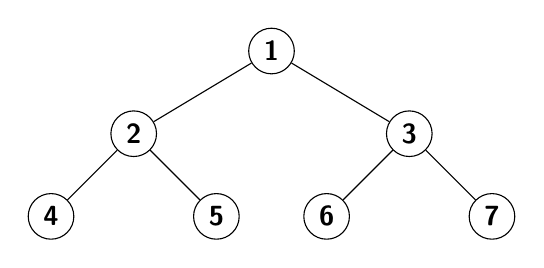
\begin{tikzpicture} [scale = 0.7,level 1/.style = {sibling distance = 5cm, level distance = 1.5cm},
						  level 2/.style = {sibling distance = 3cm}]
	\node [arn_n] {1}
	 child{ node [arn_n] {2} 
	            child{node [arn_n] {4}} 
	            child{node [arn_n] {5}}	
	      }
	 child{node [arn_n] {3} 
	            child{node [arn_n] {6}} 
	            child{node [arn_n] {7}}	
	      };
	\end{tikzpicture}

\end{center} 
\end{figure}

The same principles apply in the case of FingerTrees, which is based on a full 2-3 Tree.

I believe that the presence of these nested types makes termination checking an even harder task in many cases. The problems that occur in the implementation of the FingerTree are not limited to this context. I have provided the implementation of yet another data structure that suffers from the same limitations in Appendix \ref{app:termcheck}.

\section{2-3 Trees} 

2-3 Tree are at the basis of FingerTrees. They are rooted trees where each node has either two or three children and all leaves occur on the same level. Using nested types,as presented in the previous section, we can encode this constraint into the type of the data structure. \cite{nested}

\begin{figure} [h!]
\caption{Example 2-3 Tree}
\label{fig:23tree}
\begin{center}

	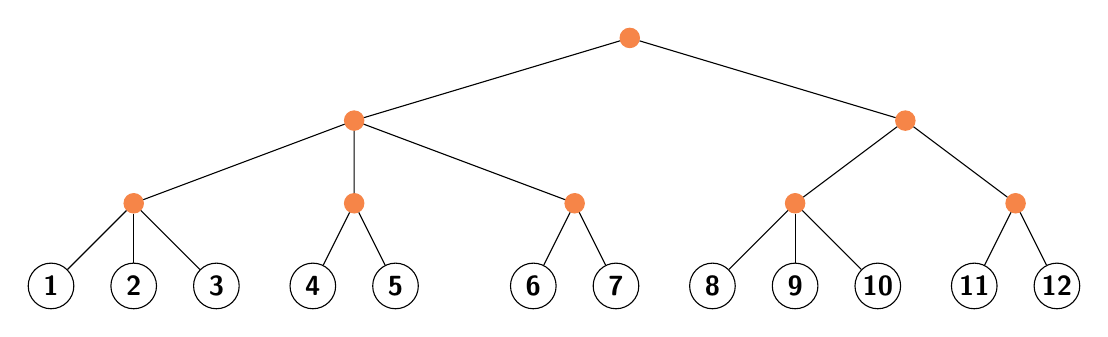
\begin{tikzpicture} [scale = 0.7,level 1/.style = {sibling distance = 10cm, level distance = 1.5cm}, 
	level 2/.style = {sibling distance = 4cm},
	level 3/.style = {sibling distance = 1.5cm}]
	\node [node] {}
	 child{ node [node] {} 
	            child{node [node] {}
	            	child{node [arn_n]{1}}
	            	child{node [arn_n]{2}}
	            	child{node [arn_n]{3}}
				} 
	            child{node [node] {}
	            	child{node [arn_n]{4}}
	            	child{node [arn_n]{5}}
	            }	
	            child{node [node] {}
	            	child{node [arn_n]{6}}
	            	child{node [arn_n]{7}}
	            }
	      }
	 child{node [node] {} 
	            child{node [node] {}
	           		child{node [arn_n]{8}}
	            	child{node [arn_n]{9}}
	            	child{node [arn_n]{10}}} 
	            child{node [node] {}
	              	child{node [arn_n]{11}}
	            	child{node [arn_n]{12}}}	
	      };
	\end{tikzpicture}

\end{center} 
\end{figure}
Instead of using the pair ($\_\times\_$) as above, we declare a new data type that can contain two as well as three elements.

\begin{code}
\\
\>\AgdaKeyword{data} \AgdaDatatype{Node} \AgdaSymbol{(}\AgdaBound{A} \AgdaSymbol{:} \AgdaPrimitiveType{Set}\AgdaSymbol{)} \AgdaSymbol{:} \AgdaPrimitiveType{Set} \AgdaKeyword{where}\<%
\\
\>[0]\AgdaIndent{2}{}\<[2]%
\>[2]\AgdaInductiveConstructor{Node2} \AgdaSymbol{:} \AgdaBound{A} \AgdaSymbol{→} \AgdaBound{A} \AgdaSymbol{→} \AgdaDatatype{Node} \AgdaBound{A}\<%
\\
\>[0]\AgdaIndent{2}{}\<[2]%
\>[2]\AgdaInductiveConstructor{Node3} \AgdaSymbol{:} \AgdaBound{A} \AgdaSymbol{→} \AgdaBound{A} \AgdaSymbol{→} \AgdaBound{A} \AgdaSymbol{→} \AgdaDatatype{Node} \AgdaBound{A}\<%
\\
\end{code}

To declare the tree, we use a nested type. The constructors are called \textit{Zero} and \textit{Succ} to signal the origin of the idea in Okasaki's numerical representations (see Appendix \ref{app:numrep})


\begin{code}
\\
\>\AgdaKeyword{data} \AgdaDatatype{Tree} \AgdaSymbol{(}\AgdaBound{A} \AgdaSymbol{:} \AgdaPrimitiveType{Set}\AgdaSymbol{)} \AgdaSymbol{:} \AgdaPrimitiveType{Set} \AgdaKeyword{where}\<%
\\
\>[0]\AgdaIndent{2}{}\<[2]%
\>[2]\AgdaInductiveConstructor{Zero} \AgdaSymbol{:} \AgdaBound{A} \AgdaSymbol{→} \AgdaDatatype{Tree} \AgdaBound{A}\<%
\\
\>[0]\AgdaIndent{2}{}\<[2]%
\>[2]\AgdaInductiveConstructor{Succ} \AgdaSymbol{:} \AgdaDatatype{Tree} \AgdaSymbol{(}\AgdaDatatype{Node} \AgdaBound{A}\AgdaSymbol{)} \AgdaSymbol{→} \AgdaDatatype{Tree} \AgdaBound{A}\<%
\\
\end{code}

As an example, Figure \ref{fig:23tree} could be written in Agda as follows (indented in an attempt to clarity):

\begin{code}
\\
\>\AgdaFunction{test-tree} \AgdaSymbol{:} \AgdaDatatype{Tree} \AgdaDatatype{ℕ}\<%
\\
\>\AgdaFunction{test-tree} \AgdaSymbol{=} \AgdaInductiveConstructor{Succ}\AgdaSymbol{(}\AgdaInductiveConstructor{Succ}\AgdaSymbol{(}\AgdaInductiveConstructor{Succ}\AgdaSymbol{(}\AgdaInductiveConstructor{Zero}\<%
\\
\>[2]\AgdaIndent{14}{}\<[14]%
\>[14]\AgdaSymbol{(}\AgdaInductiveConstructor{Node2}\<%
\\
\>[14]\AgdaIndent{18}{}\<[18]%
\>[18]\AgdaSymbol{(}\AgdaInductiveConstructor{Node3}\<%
\\
\>[18]\AgdaIndent{20}{}\<[20]%
\>[20]\AgdaSymbol{(}\AgdaInductiveConstructor{Node3} \AgdaNumber{1} \AgdaNumber{2} \AgdaNumber{3}\AgdaSymbol{)}\<%
\\
\>[18]\AgdaIndent{20}{}\<[20]%
\>[20]\AgdaSymbol{(}\AgdaInductiveConstructor{Node2} \AgdaNumber{4} \AgdaNumber{5}\AgdaSymbol{)}\<%
\\
\>[18]\AgdaIndent{20}{}\<[20]%
\>[20]\AgdaSymbol{(}\AgdaInductiveConstructor{Node2} \AgdaNumber{6} \AgdaNumber{7}\AgdaSymbol{))}\<%
\\
\>[0]\AgdaIndent{18}{}\<[18]%
\>[18]\AgdaSymbol{(}\AgdaInductiveConstructor{Node2}\<%
\\
\>[18]\AgdaIndent{20}{}\<[20]%
\>[20]\AgdaSymbol{(}\AgdaInductiveConstructor{Node3} \AgdaNumber{8} \AgdaNumber{9} \AgdaNumber{10}\AgdaSymbol{)}\<%
\\
\>[18]\AgdaIndent{20}{}\<[20]%
\>[20]\AgdaSymbol{(}\AgdaInductiveConstructor{Node2} \AgdaNumber{11} \AgdaNumber{12}\AgdaSymbol{))))))}\<%
\\
\end{code}
The number of \AgdaInductiveConstructor{Succ} nestings indicates the tree height. 
Further discussions about similar data structures can be found in \cite{nestedhinze}. Another example is present in Appendix \ref{app:termcheck}, with an emphasis on the practical difficulties of implementation in Agda.

\section{FingerTrees} 
\label{sec:fingertrees}
	FingerTrees are a data structure introduced by Ralph Hinze and Robert Patinsson\cite{fingertrees}, based on Okasaki's work in amortisation.\\
Initially designed as double-ended queues with constant amortised time append, their structure, together with the cached measurements, allow specialisation to Random Access Sequences or Priority Queues by simple instantiation.  
 
 	The underlying structure is that of a full 2-3 Tree, with labels solely at the leaves. For efficient appending, the tree is surrounded by buffers (digits) at each level. Furthermore, the data structure is accompanied by a measurement function and a binary operator, such that the reduced measures of all nodes in a sub-tree are cached in its root. These are necessary for efficient splitting (see Table \ref{tab:operations}).

\subsection{Measurements and the Monoid}
\label{sec:measure}
The versatility of the FingerTree as a data structure comes from its association with a set of measurements (\textit{V}). The \textit{measure} of the tree $\Vert ft \Vert$ is a map between  a FingerTree and an element of the set V.

The construction of this map requires two building blocks. First, we need a function that maps the elements of the FingerTree to elements of the set V, referred to as the \textbf{measurement function}. Secondly, we need the set V to be the carrier of a \textbf{Monoid}.
\begin{align*}
\intertext{That is, we pick an \textbf{operator} (in infix notation):} 
	\_\cdot\_ : (V \times V) \to V \\ 
\intertext{and an element in V, which will be called the \textbf{neutral element}, such that the next axioms hold:} 
	\forall	x \in V, \epsilon \cdot x = x  \tag{neutral-left}\\
	\forall x \in V, x \cdot \epsilon = x  \tag{neutral-right} \\
	\forall x, y,z \in V. x \cdot (y \cdot z) = (x \cdot y) \cdot z \tag{assoc} 
\end{align*}

We define the measure of the tree to be the result of recursively reducing each branch and accumulating the result using the operator ($\_\cdot\_$). At the base case, an \textbf{Empty} tree should be mapped to the \textbf{neutral element} and the \textbf{leaves} in the tree should be mapped using the \textbf{measurement function}.

A further consideration is that of efficiency. Recomputing these values would incur a linear time cost for every operation. We can amortise this cost by keeping cached measurement tags in all nodes of the tree.

\subsection{Invariants}

Achieving efficiency requires keeping two invariants on the data structure:
\begin{itemize}
	\item The tree is full and all the leaves occur on the last level. 
	\item The measurement tags are correct.
\end{itemize}

Working in Agda allows keeping these invariants solely in the type signature of the FingerTree. More specifically:
\begin{itemize}
	\item The nested typing ensures fullness of the tree.
	\item Choosing measurements as the type index ensures their correctness;
\end{itemize} 

\subsection{Previous Work}

FingerTrees have been previously implemented and proved correct. I will outline some previous results, as well as their limitations, providing more incentives for this dissertation.

\begin{itemize}
\item Basic Implementation in Agda. \\
This version can be found on GitHub.\footnote{https://github.com/fkettelhoit/agda-fingertrees}. Its mentioned intention is to closely follow the original paper. It also uses  the idea of \textit{Sizing}, although only in the type declaration (and constructors). Since the constraints do not affect functions that modify the data type, they do not really aid correctness proofs. This implementation has no proofs associated with it and didn't type check on my machine. Nonetheless, I have used it as a starting point.
\item Implementation in Coq. \\
This implementation is provided by Matthieu Souzeau\cite{coq} as a proof of concept for Russell, a Coq extension. I have drawn great inspiration from that paper, and I was particularly intrigued by a small caveat related to termination checking.

My dissertation proceeds in a similar manner, implementing the FingerTree and tackling the invariants in the same way. Additionally, I am proving further properties of the operations and presenting a working solution to the termination issue.

\item Implementation in Isabelle. \\
Another working implementation has been done in Isabelle\cite{isabelle}. However, this implementation diverges from the original specification of the data structure, removing the nesting. The two invariants that I have mentioned must be maintained explicitly, due to the lack of dependent types in Isabelle.\\ 
\end{itemize}

The fact that this data structure in both Coq and Isabelle, two established theorem provers, illustrates the complexity involved as well as the interesting nature of its particularities.

\subsection{Abstract Operations}

\begin{table}[H]
\caption{Summary of operations}
\label{tab:operations}

\begin{tabular}{c L{7cm} l}
	\hline 
	Operation & Short Description & Properties \\
	\hline
	$\_◁\_$(cons) & Appending an element at the left of the FingerTree & 
		\begin{tabular}{l}
		$\Vert x \triangleleft ft \Vert = \Vert x \Vert \cdot \Vert ft \Vert $ \\
		$ toList(x \triangleleft ft) = x ∷ toList ft$ \\
		\end{tabular}\\
	\hline
	snoc & Appending an element at the right of the FingerTree & 
		\begin{tabular}{l}
		$\Vert x \triangleright ft \Vert = \Vert ft \Vert \cdot \Vert x \Vert $ \\
		$ toList(x \triangleright ft) = toList ft ++ [ x ] $ \\
		\end{tabular}\\
	\hline	
	viewL & Deconstructing a FingerTree into its first element and the rest of the elements reorganised as a FingerTree & 
		\begin{tabular}{l}
		$\Vert viewL ft \Vert = \Vert ft \Vert $ \\
		$ toList(viewL ft) = toList ft$ \\
		\end{tabular}\\
	\hline
	viewR & Deconstructing a FingerTree into its last element and the rest of the elements reorganised as a FingerTree & 
		\begin{tabular}{l}
		$\Vert viewR ft \Vert = \Vert ft \Vert $ \\
		$ toList(viewR ft) = toList ft$ \\
		\end{tabular}\\
	\hline
	foldL-ft & Similar to the same operation on Lists, equivalent to mentally replacing all the nodes with a call to a given function & 
		\begin{tabular}{l}
		$ foldL-ft(i, f, ft) = foldl(i, f, toList ft) $ \\
		$ foldL-ft(\epsilon, foldfun, ft) = \Vert ft \Vert $ \\
		where \\
		$ foldfun(a, b) = \Vert a \Vert \cdot b $ \\ 
		\end{tabular}\\
	\hline
	split & Extract an arbitrary element, given by a predicate function \textit{P} and reconstruct the left and right remaining element into two FingerTrees &
	\begin{tabular}{l}
		$ \Vert split (i, P, ft) \Vert = \Vert ft \Vert $ \\
	\end{tabular}\\
	\hline
	
\end{tabular}

\end{table}

Some of the properties on the rightmost column are  presented in the implementation. There are properties which could not be proven due to problems with the \AgdaKeyword{with} operator, which I  present in section \ref{sec:with}.

The properties related to size ($\Vert\_\Vert$) are proven 'internally', as part of the implementation. The others are proven 'externally', by defining terms of types that express those properties. 

\section{Starting Point}

At the beginning of this project, I had no previous knowledge of:
\begin{itemize}
 \item Agda or Haskell - although I did have experience with functional programming languages from the Foundations of Computer Science course.
 \item Formal verification of computer programs.
 \item FingerTrees and other advanced functional data structures.
\end{itemize}

Some relevant material was present in \textit{Logic and Proof} (Larry Paulson) and \textit{Types} (Andrew Pitts), as well as some parts from Discrete Mathematics (Marcelo Fiore) and Computation Theory (Andrew Pitts). 

\chapter{Implementation}

\section{FingerTrees - Implementation}

The previous section has provided an abstract representation of FingerTrees, as well as introduced the prerequisites for writing an implementation in Agda. In the following, I will provide implementations of the constructors and operations described in Table \ref{tab:operations} and present proofs of correctness. 

\subsection{Data type declaration}
\label{sec:ftdecl}
The FingerTree is originally polymorphic in two types:
\begin{itemize}
\item \textbf{A}: the type of elements that are contained in the FingerTree.
\item \textbf{V}: the type of measures. 
\end{itemize} 

In order to to mimic Haskell's typeclasses, I have carried around, for each A and V, two records:

\begin{itemize} 
\item \textbf{Monoid\footnote{see AlgebraStructures.agda} V}: which contains a neutral element(\textbf{ε}), a binary operator(\textbf{$∙$}), the monoid axioms and a comparison operator.
\item \textbf{Measured A V}: which consists of a norm function  :  \textbf{$\Vert\_\Vert : \nolinebreak A \rightarrow V$}.
\end{itemize} 

\textbf{Node} corresponds to nodes in the underlying 2-3 Tree implementation, having two constructors for two and respectively three items. Moreover, \textbf{Node}s can only be constructed if provided with a measurement tag and a correctness proof.
  
\begin{code}
\\
\>\AgdaKeyword{data} \AgdaDatatype{Node} \AgdaSymbol{\{}\AgdaBound{a}\AgdaSymbol{\}} \AgdaSymbol{(}\AgdaBound{A} \AgdaSymbol{:} \AgdaPrimitiveType{Set} \AgdaBound{a}\AgdaSymbol{)(}\AgdaBound{V} \AgdaSymbol{:} \AgdaPrimitiveType{Set} \AgdaBound{a} \AgdaSymbol{)}\<%
\\
\>[0]\AgdaIndent{10}{}\<[10]%
\>[10]\AgdaSymbol{⦃} \AgdaBound{mo} \AgdaSymbol{:} \AgdaRecord{Monoid} \AgdaBound{V} \AgdaSymbol{⦄}\<%
\\
\>[0]\AgdaIndent{10}{}\<[10]%
\>[10]\AgdaSymbol{⦃} \AgdaBound{m} \AgdaSymbol{:} \AgdaRecord{Measured} \AgdaBound{A} \AgdaBound{V} \AgdaSymbol{⦄} \AgdaSymbol{:} \AgdaPrimitiveType{Set} \AgdaBound{a} \AgdaKeyword{where}\<%
\\
\>[0]\AgdaIndent{2}{}\<[2]%
\>[2]\AgdaInductiveConstructor{Node2} \AgdaSymbol{:} \AgdaSymbol{(}\AgdaBound{v} \AgdaSymbol{:} \AgdaBound{V}\AgdaSymbol{)}\<%
\\
\>[2]\AgdaIndent{8}{}\<[8]%
\>[8]\AgdaSymbol{→} \AgdaSymbol{(}\AgdaBound{x} \AgdaSymbol{:} \AgdaBound{A}\AgdaSymbol{)} \AgdaSymbol{→} \AgdaSymbol{(}\AgdaBound{y} \AgdaSymbol{:} \AgdaBound{A}\AgdaSymbol{)}\<%
\\
\>[2]\AgdaIndent{8}{}\<[8]%
\>[8]\AgdaSymbol{→} \<[11]%
\>[11]\AgdaSymbol{(}\AgdaBound{v} \AgdaDatatype{≡} \AgdaField{∥} \AgdaBound{x} \AgdaField{∥} \AgdaField{∙} \AgdaField{∥} \AgdaBound{y} \AgdaField{∥}\AgdaSymbol{)}\<%
\\
\>[2]\AgdaIndent{8}{}\<[8]%
\>[8]\AgdaSymbol{→} \AgdaDatatype{Node} \AgdaBound{A} \AgdaBound{V}\<%
\\
\>[0]\AgdaIndent{2}{}\<[2]%
\>[2]\AgdaInductiveConstructor{Node3} \AgdaSymbol{:} \AgdaSymbol{(}\AgdaBound{v} \AgdaSymbol{:} \AgdaBound{V}\AgdaSymbol{)}\<%
\\
\>[2]\AgdaIndent{8}{}\<[8]%
\>[8]\AgdaSymbol{→} \AgdaSymbol{(}\AgdaBound{x} \AgdaSymbol{:} \AgdaBound{A}\AgdaSymbol{)} \AgdaSymbol{→} \AgdaSymbol{(}\AgdaBound{y} \AgdaSymbol{:} \AgdaBound{A}\AgdaSymbol{)} \AgdaSymbol{→} \AgdaSymbol{(}\AgdaBound{z} \AgdaSymbol{:} \AgdaBound{A}\AgdaSymbol{)}\<%
\\
\>[2]\AgdaIndent{8}{}\<[8]%
\>[8]\AgdaSymbol{→} \AgdaSymbol{(}\AgdaBound{v} \AgdaDatatype{≡} \AgdaField{∥} \AgdaBound{x} \AgdaField{∥} \AgdaField{∙} \AgdaField{∥} \AgdaBound{y} \AgdaField{∥} \AgdaField{∙} \AgdaField{∥} \AgdaBound{z} \AgdaField{∥}\AgdaSymbol{)}\<%
\\
\>[2]\AgdaIndent{8}{}\<[8]%
\>[8]\AgdaSymbol{→} \AgdaDatatype{Node} \AgdaBound{A} \AgdaBound{V}\<%
\\
\end{code}
\textbf{Digit}s were presented in the original paper as lists, but this definition limits them to having one to four elements.

\begin{code}
\\
\>\AgdaKeyword{data} \AgdaDatatype{Digit} \AgdaSymbol{\{}\AgdaBound{a}\AgdaSymbol{\}} \AgdaSymbol{(}\AgdaBound{A} \AgdaSymbol{:} \AgdaPrimitiveType{Set} \AgdaBound{a}\AgdaSymbol{):} \AgdaPrimitiveType{Set} \AgdaBound{a} \AgdaKeyword{where}\<%
\\
\>[0]\AgdaIndent{2}{}\<[2]%
\>[2]\AgdaInductiveConstructor{One} \<[8]%
\>[8]\AgdaSymbol{:} \AgdaBound{A} \AgdaSymbol{→} \AgdaDatatype{Digit} \AgdaBound{A}\<%
\\
\>[0]\AgdaIndent{2}{}\<[2]%
\>[2]\AgdaInductiveConstructor{Two} \<[8]%
\>[8]\AgdaSymbol{:} \AgdaBound{A} \AgdaSymbol{→} \AgdaBound{A} \AgdaSymbol{→} \AgdaDatatype{Digit} \AgdaBound{A}\<%
\\
\>[0]\AgdaIndent{2}{}\<[2]%
\>[2]\AgdaInductiveConstructor{Three} \AgdaSymbol{:} \AgdaBound{A} \AgdaSymbol{→} \AgdaBound{A} \AgdaSymbol{→} \AgdaBound{A} \AgdaSymbol{→} \AgdaDatatype{Digit} \AgdaBound{A}\<%
\\
\>[0]\AgdaIndent{2}{}\<[2]%
\>[2]\AgdaInductiveConstructor{Four} \<[8]%
\>[8]\AgdaSymbol{:} \AgdaBound{A} \AgdaSymbol{→} \AgdaBound{A} \AgdaSymbol{→} \AgdaBound{A} \AgdaSymbol{→} \AgdaBound{A} \AgdaSymbol{→} \AgdaDatatype{Digit} \AgdaBound{A}\<%
\\
\end{code}

Finally, the \textbf{FingerTree} is a family of types, indexed by a measurement $\mu$. The measurement's correctness is enforced in all constructors. Note the nested type and the universal quantification over possible sizes for the recursive call. Apart from the measurement indexing, the rest corresponds to the original paper \cite{fingertrees}.

\begin{code}
\\
\>\AgdaKeyword{data} \AgdaDatatype{FingerTree} \AgdaSymbol{\{}\AgdaBound{a}\AgdaSymbol{\}} \AgdaSymbol{(}\AgdaBound{A} \AgdaSymbol{:} \AgdaPrimitiveType{Set} \AgdaBound{a}\AgdaSymbol{)(}\AgdaBound{V} \AgdaSymbol{:} \AgdaPrimitiveType{Set} \AgdaBound{a}\AgdaSymbol{)}\<%
\\
\>[2]\AgdaIndent{16}{}\<[16]%
\>[16]\AgdaSymbol{⦃} \AgdaBound{mo} \AgdaSymbol{:} \AgdaRecord{Monoid} \AgdaBound{V} \AgdaSymbol{⦄}\<%
\\
\>[2]\AgdaIndent{16}{}\<[16]%
\>[16]\AgdaSymbol{⦃} \AgdaBound{m} \AgdaSymbol{:} \AgdaRecord{Measured} \AgdaBound{A} \AgdaBound{V} \AgdaSymbol{⦄} \AgdaSymbol{:}\<%
\\
\>[2]\AgdaIndent{16}{}\<[16]%
\>[16]\AgdaSymbol{\{}\AgdaBound{μ} \AgdaSymbol{:} \AgdaBound{V}\AgdaSymbol{\}} \AgdaSymbol{→} \AgdaPrimitiveType{Set} \AgdaBound{a} \AgdaKeyword{where}\<%
\\
\>[0]\AgdaIndent{2}{}\<[2]%
\>[2]\AgdaInductiveConstructor{Empty} \<[9]%
\>[9]\AgdaSymbol{:} \<[12]%
\>[12]\AgdaDatatype{FingerTree} \AgdaBound{A} \AgdaBound{V} \AgdaSymbol{\{}\AgdaField{ε}\AgdaSymbol{\}}\<%
\\
\>[0]\AgdaIndent{2}{}\<[2]%
\>[2]\AgdaInductiveConstructor{Single} \AgdaSymbol{:} \<[12]%
\>[12]\AgdaSymbol{(}\AgdaBound{e} \AgdaSymbol{:} \AgdaBound{A}\AgdaSymbol{)} \AgdaSymbol{→} \AgdaDatatype{FingerTree} \AgdaBound{A} \AgdaBound{V} \AgdaSymbol{\{}\AgdaField{∥} \AgdaBound{e} \AgdaField{∥}\AgdaSymbol{\}}\<%
\\
\>[0]\AgdaIndent{2}{}\<[2]%
\>[2]\AgdaInductiveConstructor{Deep} \<[9]%
\>[9]\AgdaSymbol{:} \<[12]%
\>[12]\AgdaSymbol{\{}\AgdaBound{s} \AgdaSymbol{:} \AgdaBound{V}\AgdaSymbol{\}}\<%
\\
\>[2]\AgdaIndent{10}{}\<[10]%
\>[10]\AgdaSymbol{→} \AgdaSymbol{(}\AgdaBound{pr} \AgdaSymbol{:} \AgdaDatatype{Digit} \AgdaBound{A}\AgdaSymbol{)}\<%
\\
\>[2]\AgdaIndent{10}{}\<[10]%
\>[10]\AgdaSymbol{→} \AgdaDatatype{FingerTree} \AgdaSymbol{(}\AgdaDatatype{Node} \AgdaBound{A} \AgdaBound{V}\AgdaSymbol{)} \AgdaBound{V} \AgdaSymbol{\{}\AgdaBound{s}\AgdaSymbol{\}}\<%
\\
\>[2]\AgdaIndent{10}{}\<[10]%
\>[10]\AgdaSymbol{→} \AgdaSymbol{(}\AgdaBound{sf} \AgdaSymbol{:} \AgdaDatatype{Digit} \AgdaBound{A}\AgdaSymbol{)}\<%
\\
\>[2]\AgdaIndent{10}{}\<[10]%
\>[10]\AgdaSymbol{→} \AgdaDatatype{FingerTree} \AgdaBound{A} \AgdaBound{V} \AgdaSymbol{\{}\AgdaFunction{measure-digit} \AgdaBound{pr} \AgdaField{∙} \AgdaBound{s} \AgdaField{∙} \AgdaFunction{measure-digit} \AgdaBound{sf}\AgdaSymbol{\}}\<%
\\
\end{code}

\subparagraph{Smart Constructors.}
We also build smart constructors that fill in the measurement, when provided with the appropriate number of elements:

\begin{code}
\\
\>\AgdaFunction{node2} \AgdaSymbol{:} \AgdaSymbol{∀} \AgdaSymbol{\{}\AgdaBound{a}\AgdaSymbol{\}} \AgdaSymbol{\{}\AgdaBound{A} \AgdaSymbol{:} \AgdaPrimitiveType{Set} \AgdaBound{a}\AgdaSymbol{\}\{}\AgdaBound{V} \AgdaSymbol{:} \AgdaPrimitiveType{Set} \AgdaBound{a} \AgdaSymbol{\}}\<%
\\
\>[0]\AgdaIndent{8}{}\<[8]%
\>[8]\AgdaSymbol{⦃} \AgdaBound{mo} \AgdaSymbol{:} \AgdaRecord{Monoid} \AgdaBound{V} \AgdaSymbol{⦄}\<%
\\
\>[0]\AgdaIndent{8}{}\<[8]%
\>[8]\AgdaSymbol{⦃} \AgdaBound{m} \AgdaSymbol{:} \AgdaRecord{Measured} \AgdaBound{A} \AgdaBound{V} \AgdaSymbol{⦄}\<%
\\
\>[0]\AgdaIndent{8}{}\<[8]%
\>[8]\AgdaSymbol{→} \AgdaBound{A} \AgdaSymbol{→} \AgdaBound{A} \AgdaSymbol{→} \AgdaDatatype{Node} \AgdaBound{A} \AgdaBound{V}\<%
\\
\>\AgdaFunction{node2} \AgdaBound{x} \AgdaBound{y} \AgdaSymbol{=} \AgdaInductiveConstructor{Node2} \AgdaSymbol{(}\AgdaField{∥} \AgdaBound{x} \AgdaField{∥} \AgdaField{∙} \AgdaField{∥} \AgdaBound{y} \AgdaField{∥}\AgdaSymbol{)} \AgdaBound{x} \AgdaBound{y} \AgdaInductiveConstructor{refl}\<%
\\
%
\\
\>\AgdaFunction{node3} \AgdaSymbol{:} \AgdaSymbol{∀} \AgdaSymbol{\{}\AgdaBound{a}\AgdaSymbol{\}} \AgdaSymbol{\{}\AgdaBound{A} \AgdaSymbol{:} \AgdaPrimitiveType{Set} \AgdaBound{a}\AgdaSymbol{\}\{}\AgdaBound{V} \AgdaSymbol{:} \AgdaPrimitiveType{Set} \AgdaBound{a} \AgdaSymbol{\}}\<%
\\
\>[0]\AgdaIndent{8}{}\<[8]%
\>[8]\AgdaSymbol{⦃} \AgdaBound{mo} \AgdaSymbol{:} \AgdaRecord{Monoid} \AgdaBound{V} \AgdaSymbol{⦄}\<%
\\
\>[0]\AgdaIndent{8}{}\<[8]%
\>[8]\AgdaSymbol{⦃} \AgdaBound{m} \AgdaSymbol{:} \AgdaRecord{Measured} \AgdaBound{A} \AgdaBound{V} \AgdaSymbol{⦄}\<%
\\
\>[0]\AgdaIndent{8}{}\<[8]%
\>[8]\AgdaSymbol{→} \AgdaBound{A} \AgdaSymbol{→} \AgdaBound{A} \AgdaSymbol{→} \AgdaBound{A} \AgdaSymbol{→} \AgdaDatatype{Node} \AgdaBound{A} \AgdaBound{V}\<%
\\
\>\AgdaFunction{node3} \AgdaBound{x} \AgdaBound{y} \AgdaBound{z} \AgdaSymbol{=} \AgdaInductiveConstructor{Node3} \AgdaSymbol{(}\AgdaField{∥} \AgdaBound{x} \AgdaField{∥} \AgdaField{∙} \AgdaField{∥} \AgdaBound{y} \AgdaField{∥} \AgdaField{∙} \AgdaField{∥} \AgdaBound{z} \AgdaField{∥}\AgdaSymbol{)} \AgdaBound{x} \AgdaBound{y} \AgdaBound{z} \AgdaInductiveConstructor{refl}\<%
\\
\end{code}

Considering Figure, \ref{fig:ftex1}, I have colour-coded the nodes as follows:
\begin{table}[h!]
\centering
\begin{tabular}{c c}
Symbol & Constructor \\ 
\hline

\begin{tikzpicture} [scale = 0.7,level 1/.style = {sibling distance = 2cm, level distance = 1.5cm}]		  
		\node [deep] {};
\end{tikzpicture} & Deep \\
 

\begin{tikzpicture} [scale = 0.7,level 1/.style = {sibling distance = 2cm, level distance = 1.5cm}]		  
		\node [node] {};
\end{tikzpicture} & Node \\
\begin{tikzpicture} [scale = 0.7,level 1/.style = {sibling distance = 2cm, level distance = 1.5cm}]		  
		\node [digit] {∙ ∙ ∙};
\end{tikzpicture} & Digit (of various lengths) \\


\begin{tikzpicture} [scale = 0.7,level 1/.style = {sibling distance = 2cm, level distance = 1.5cm}]		  
		\node [leaf] {};
\end{tikzpicture} & Empty \\
\hline
\end{tabular}
\end{table}


\subsection{Indexing on the measurement}

The reason for indexing on the measurement is twofold. Firstly, we index on the measurement in order to verify the correctness of the measurement in operations such as appending an element or splitting. Secondly, the index was chosen in order to allow a \textit{Sizing} that depends on all elements in the FingerTree. 

Consider a sizing that would take into account the shape of the tree only (as it is the case of Size described previously). 

\begin{figure}[h!]
\centering 
	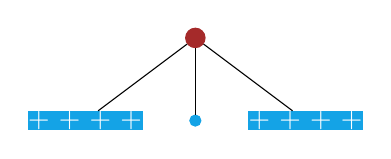
\begin{tikzpicture} [scale = 0.7,level 1/.style = {sibling distance = 2cm, level distance = 1.5cm},					  
		level 2/.style = {sibling distance = 4cm, level distance = 1.5cm},
		level 3/.style = {sibling distance = 2cm, level distance = 1.5cm}]
		\node [deep] {}
		 child{node [digit] {+ + + +} 	
		      }
		 child{node [leaf] {}}
		 child{node [digit] {+ + + +}	
		      };
	\end{tikzpicture}
	\caption{Bigger FingerTree}
	\label{fig:ftex2}
	\vspace{3mm}
	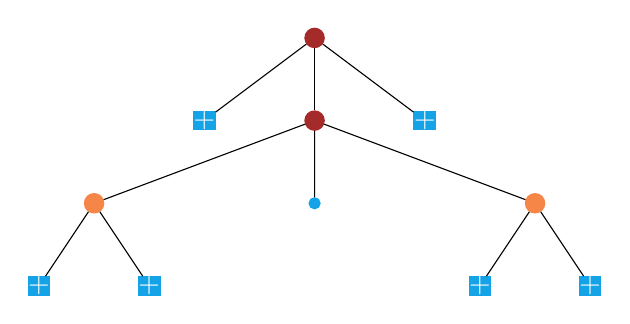
\begin{tikzpicture} [scale = 0.7,level 1/.style = {sibling distance = 2cm, level distance = 1.5cm},					  
		level 2/.style = {sibling distance = 4cm, level distance = 1.5cm},
		level 3/.style = {sibling distance = 2cm, level distance = 1.5cm}]
		\node [deep] {}
		 child{node [digit] {+} 	
		      }
		 child{node [deep] {}
		 		child{node [node] {}
		 				child{node [digit] {+}}
		 				child{node [digit] {+}}
		 			}
			 	child{node [leaf] {}}
		 		child{node [node] {}
		 				child{node [digit] {+}} 
		 				child{node [digit] {+}}
		 			}
		 	 } 
		 child{node [digit] {+}	
		      };
	\end{tikzpicture}
	\caption{Smaller FingerTree}
	\label{fig:ftex3}
\end{figure} 

In Figures \ref{fig:ftex2} and \ref{fig:ftex3}, it is ambiguous which of the two trees should be considered to have a bigger size. \textit{Size} implements a partial order between data types, with no definite reference points, whereas here we are concerned with an absolute order. I will show in section \ref{sec:viewLsize} how using \textit{Sized Types} can impede the implementation of the \AgdaFunction{viewL} operation.
 
\indent As suggested by Matthew Souzeau \cite{coq}, a sizing that reflects the number of elements is ideal. We can use the already existing measurement index to achieve this goal.

Having completed the declaration of the data type, I will next present the implementation of the operations in Table \ref{tab:operations}, with associated proofs and discussions.

\subsection{\AgdaFunction{\_◁\_}(Cons) and \textit{Snoc}}

\AgdaFunction{\_◁\_}(cons) is the operator that appends an element to the left of the FingerTree. 

The implementation is straightforward if there is room in the leftmost digit. Otherwise, we have to recursively insert and reform parts of the FingerTree.

Ultimately, for correctness, we are concerned with whether the output tree is a correct FingerTree that has a correct measurement. 
\begin{align*}
\intertext{That is, by inserting an element x,}
	\Vert x \triangleleft ft \Vert = \Vert x \Vert \cdot \Vert ft \Vert
\end{align*}
\begin{figure}[h!]
\centering 
\subfloat[Before Cons]
{
	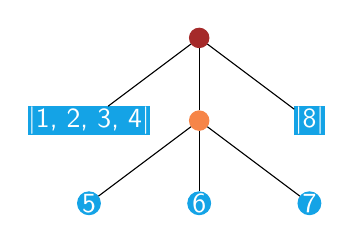
\begin{tikzpicture} [scale = 0.7,level 1/.style = {sibling distance = 2cm, level distance = 1.5cm},					  
		level 2/.style = {sibling distance = 2cm, level distance = 1.5cm},
		level 3/.style = {sibling distance = 2cm, level distance = 1.5cm}]
		\node [deep] {}
		 child{node [digit] {$|$1, 2, 3, 4$|$} 	
		      }
		 child{node [node] {}
				child {node [leaf] {5}}
				child {node [leaf] {6}}
				child {node [leaf] {7}}
		}
		 child{node [digit] {$|$8$|$}	
		      };
	\end{tikzpicture}
}
\qquad
\subfloat[After Cons]
{
	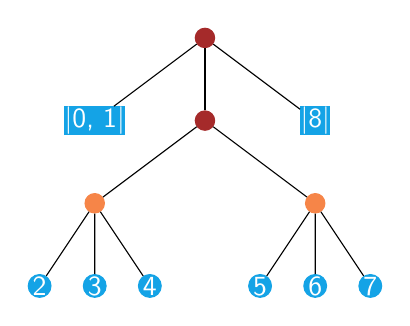
\begin{tikzpicture} [scale = 0.7,level 1/.style = {sibling distance = 2cm, level distance = 1.5cm},					  
		level 2/.style = {sibling distance = 4cm, level distance = 1.5cm},
		level 3/.style = {sibling distance = 1cm, level distance = 1.5cm}]
		\node [deep] {}
		 child{node [digit] {$|$0, 1$|$} 	
		      }
		 child{node [deep] {}
		 		child{node [node] {}
		 				child{node [leaf] {2}}
		 				child{node [leaf] {3}}
		 				child{node [leaf] {4}}
		 			}
			 	child{node [node] {}
		 				child{node [leaf] {5}} 
		 				child{node [leaf] {6}}
		 				child{node [leaf] {7}}
		 			}
		 	 } 
		 child{node [digit] {$|$8$|$}	
		      };
	\end{tikzpicture}
}
	\caption{Recursive \AgdaFunction{\_◁\_}(cons) operation}
	\label{fig:ftex3}
\end{figure}

\begin{code}
\\
\\
\>\AgdaFunction{\_◁\_} \AgdaSymbol{:} \AgdaSymbol{∀} \AgdaSymbol{\{}\AgdaBound{a}\AgdaSymbol{\}} \AgdaSymbol{\{}\AgdaBound{A} \AgdaSymbol{:} \AgdaPrimitiveType{Set} \AgdaBound{a}\AgdaSymbol{\}} \AgdaSymbol{\{}\AgdaBound{V} \AgdaSymbol{:} \AgdaPrimitiveType{Set} \AgdaBound{a}\AgdaSymbol{\}}\<%
\\
\>[2]\AgdaIndent{6}{}\<[6]%
\>[6]\AgdaSymbol{⦃} \AgdaBound{mo} \AgdaSymbol{:} \AgdaRecord{Monoid} \AgdaBound{V} \AgdaSymbol{⦄}\<%
\\ 
\>[2]\AgdaIndent{6}{}\<[6]%
\>[6]\AgdaSymbol{⦃} \AgdaBound{m} \AgdaSymbol{:} \AgdaRecord{Measured} \AgdaBound{A} \AgdaBound{V} \AgdaSymbol{⦄}\<%
\\
\>[2]\AgdaIndent{6}{}\<[6]%
\>[6]\AgdaSymbol{\{}\AgdaBound{s} \AgdaSymbol{:} \AgdaBound{V}\AgdaSymbol{\}}\<%
\\
\>[2]\AgdaIndent{6}{}\<[6]%
\>[6]\AgdaSymbol{→} \AgdaSymbol{(}\AgdaBound{x} \AgdaSymbol{:} \AgdaBound{A}\AgdaSymbol{)}\<%
\\
\>[2]\AgdaIndent{6}{}\<[6]%
\>[6]\AgdaSymbol{→} \AgdaDatatype{FingerTree} \AgdaBound{A} \AgdaBound{V} \AgdaSymbol{⦃} \AgdaBound{mo} \AgdaSymbol{⦄} \AgdaSymbol{⦃} \AgdaBound{m} \AgdaSymbol{⦄} \AgdaSymbol{\{}\AgdaBound{s}\AgdaSymbol{\}}\<%
\\
\>[2]\AgdaIndent{6}{}\<[6]%
\>[6]\AgdaSymbol{→} \AgdaDatatype{FingerTree} \AgdaBound{A} \AgdaBound{V} \AgdaSymbol{⦃} \AgdaBound{mo} \AgdaSymbol{⦄} \AgdaSymbol{⦃} \AgdaBound{m} \AgdaSymbol{⦄} \AgdaSymbol{\{}\AgdaField{∥} \AgdaBound{x} \AgdaField{∥} \AgdaField{∙} \AgdaBound{s}\AgdaSymbol{\}}\<%
\\
\end{code}
Each case in the definition is accompanied by a proof that the measurement of the output FingerTree is correct with respect to the definition. The result of the function is presented after the equal sign (=), and the \AgdaKeyword{rewrite} clause contains evidence for the type-checker that the declaration respects the type signature.

Also note that the first two cases had to be written in prefix notation, damaging readability. The reasons for this are that the bare type information was not sufficient for performing inference, and I had to manually tag the operations and make the implicit arguments explicit.

\begin{code} 
\\
\>\AgdaFunction{\_◁\_} \AgdaSymbol{\{}\AgdaBound{l}\AgdaSymbol{\}} \AgdaSymbol{\{}\AgdaBound{A}\AgdaSymbol{\}} \AgdaSymbol{\{}\AgdaBound{V}\AgdaSymbol{\}} \AgdaSymbol{⦃} \AgdaBound{mo} \AgdaSymbol{⦄} \AgdaBound{a} \AgdaInductiveConstructor{Empty}\<%
\\
\>[0]\AgdaIndent{2}{}\<[2]%
\>[2]\AgdaKeyword{rewrite} \AgdaSymbol{(}\AgdaField{Monoid.ε-right} \AgdaBound{mo}\AgdaSymbol{)} \AgdaField{∥} \AgdaBound{a} \AgdaField{∥}\<%
\\
\>[0]\AgdaIndent{2}{}\<[2]%
\>[2]\AgdaSymbol{=} \AgdaInductiveConstructor{Single} \AgdaSymbol{\{}\AgdaBound{l}\AgdaSymbol{\}\{}\AgdaBound{A}\AgdaSymbol{\}\{}\AgdaBound{V}\AgdaSymbol{\}} \AgdaBound{a}\<%
\\
\>\AgdaFunction{\_◁\_} \AgdaSymbol{\{}\AgdaBound{l}\AgdaSymbol{\}} \AgdaSymbol{\{}\AgdaBound{A}\AgdaSymbol{\}} \AgdaSymbol{\{}\AgdaBound{V}\AgdaSymbol{\}} \AgdaSymbol{⦃} \AgdaBound{mo} \AgdaSymbol{⦄} \AgdaSymbol{⦃} \AgdaBound{m} \AgdaSymbol{⦄} \AgdaSymbol{\{}\AgdaSymbol{.(}\AgdaField{∥} \AgdaBound{e} \AgdaField{∥}\AgdaSymbol{)}\AgdaSymbol{\}} \AgdaBound{a} \AgdaSymbol{(}\AgdaInductiveConstructor{Single} \AgdaBound{e}\AgdaSymbol{)}\<%
\\
\>[0]\AgdaIndent{2}{}\<[2]%
\>[2]\AgdaKeyword{rewrite} \AgdaFunction{assoc-lemma1} \AgdaSymbol{⦃} \AgdaBound{mo} \AgdaSymbol{⦄} \AgdaSymbol{⦃} \AgdaBound{m} \AgdaSymbol{⦄} \AgdaBound{a} \AgdaBound{e}\<%
\\
\>[0]\AgdaIndent{2}{}\<[2]%
\>[2]\AgdaSymbol{=} \AgdaInductiveConstructor{Deep} \AgdaSymbol{(}\AgdaInductiveConstructor{One} \AgdaBound{a}\AgdaSymbol{)} \AgdaInductiveConstructor{Empty} \AgdaSymbol{(}\AgdaInductiveConstructor{One} \AgdaBound{e}\AgdaSymbol{)}\<%
\\
\>\AgdaBound{a} \AgdaFunction{◁} \AgdaInductiveConstructor{Deep} \AgdaSymbol{(}\AgdaInductiveConstructor{One} \AgdaBound{b}\AgdaSymbol{)} \AgdaBound{ft} \AgdaBound{sf}\<%
\\
\>[0]\AgdaIndent{2}{}\<[2]%
\>[2]\AgdaKeyword{rewrite} \AgdaField{∙-assoc} \AgdaSymbol{(}\AgdaField{∥} \AgdaBound{a} \AgdaField{∥}\AgdaSymbol{)} \AgdaSymbol{(}\AgdaField{∥} \AgdaBound{b} \AgdaField{∥}\AgdaSymbol{)} \AgdaSymbol{(}\AgdaFunction{measure-tree} \AgdaBound{ft} \AgdaField{∙} \AgdaFunction{measure-digit} \AgdaBound{sf}\AgdaSymbol{)}\<%
\\
\>[0]\AgdaIndent{2}{}\<[2]%
\>[2]\AgdaSymbol{=} \AgdaInductiveConstructor{Deep} \AgdaSymbol{(}\AgdaInductiveConstructor{Two} \AgdaBound{a} \AgdaBound{b}\AgdaSymbol{)} \AgdaBound{ft} \AgdaBound{sf}\<%
\\
\>\AgdaBound{a} \AgdaFunction{◁} \AgdaInductiveConstructor{Deep} \AgdaSymbol{(}\AgdaInductiveConstructor{Two} \AgdaBound{b} \AgdaBound{c}\AgdaSymbol{)} \AgdaBound{ft} \AgdaBound{sf}\<%
\\
\>[0]\AgdaIndent{2}{}\<[2]%
\>[2]\AgdaKeyword{rewrite} \AgdaField{∙-assoc} \AgdaSymbol{(}\AgdaField{∥} \AgdaBound{a} \AgdaField{∥}\AgdaSymbol{)} \AgdaSymbol{(}\AgdaField{∥} \AgdaBound{b} \AgdaField{∥} \AgdaField{∙} \AgdaField{∥} \AgdaBound{c} \AgdaField{∥}\AgdaSymbol{)} \AgdaSymbol{(}\AgdaFunction{measure-tree} \AgdaBound{ft} \AgdaField{∙} \AgdaFunction{measure-digit} \AgdaBound{sf}\AgdaSymbol{)}\<%
\\
\>[0]\AgdaIndent{2}{}\<[2]%
\>[2]\AgdaSymbol{=} \AgdaInductiveConstructor{Deep} \AgdaSymbol{(}\AgdaInductiveConstructor{Three} \AgdaBound{a} \AgdaBound{b} \AgdaBound{c}\AgdaSymbol{)} \AgdaBound{ft} \AgdaBound{sf}\<%
\\
\>\AgdaBound{a} \AgdaFunction{◁} \AgdaInductiveConstructor{Deep} \AgdaSymbol{(}\AgdaInductiveConstructor{Three} \AgdaBound{b} \AgdaBound{c} \AgdaBound{d}\AgdaSymbol{)} \AgdaBound{ft} \AgdaBound{sf}\<%
\\
\>[0]\AgdaIndent{2}{}\<[2]%
\>[2]\AgdaKeyword{rewrite} \AgdaField{∙-assoc} \AgdaSymbol{(}\AgdaField{∥} \AgdaBound{a} \AgdaField{∥}\AgdaSymbol{)} \AgdaSymbol{(}\AgdaField{∥} \AgdaBound{b} \AgdaField{∥} \AgdaField{∙} \AgdaField{∥} \AgdaBound{c} \AgdaField{∥} \AgdaField{∙} \AgdaField{∥} \AgdaBound{d} \AgdaField{∥}\AgdaSymbol{)} \AgdaSymbol{(}\AgdaFunction{measure-tree} \AgdaBound{ft} \AgdaField{∙} \AgdaFunction{measure-digit} \AgdaBound{sf}\AgdaSymbol{)}\<%
\\
\>[0]\AgdaIndent{2}{}\<[2]%
\>[2]\AgdaSymbol{=} \AgdaInductiveConstructor{Deep} \AgdaSymbol{(}\AgdaInductiveConstructor{Four} \AgdaBound{a} \AgdaBound{b} \AgdaBound{c} \AgdaBound{d}\AgdaSymbol{)} \AgdaBound{ft} \AgdaBound{sf}\<%
\\
\>\AgdaBound{a} \AgdaFunction{◁} \AgdaInductiveConstructor{Deep} \AgdaSymbol{(}\AgdaInductiveConstructor{Four} \AgdaBound{b} \AgdaBound{c} \AgdaBound{d} \AgdaBound{e}\AgdaSymbol{)} \AgdaBound{ft} \AgdaBound{sf}\<%
\\
\>[0]\AgdaIndent{2}{}\<[2]%
\>[2]\AgdaKeyword{rewrite} \AgdaFunction{assoc-lemma2} \AgdaBound{a} \AgdaBound{b} \AgdaBound{c} \AgdaBound{d} \AgdaBound{e} \AgdaSymbol{(}\AgdaFunction{measure-tree} \AgdaBound{ft}\AgdaSymbol{)} \AgdaSymbol{(}\AgdaFunction{measure-digit} \AgdaBound{sf}\AgdaSymbol{)}\<%
\\
\>[0]\AgdaIndent{2}{}\<[2]%
\>[2]\AgdaSymbol{=} \AgdaInductiveConstructor{Deep} \AgdaSymbol{(}\AgdaInductiveConstructor{Two} \AgdaBound{a} \AgdaBound{b}\AgdaSymbol{)} \AgdaSymbol{((}\AgdaFunction{node3} \AgdaBound{c} \AgdaBound{d} \AgdaBound{e}\AgdaSymbol{)} \AgdaFunction{◁} \AgdaBound{ft}\AgdaSymbol{)} \AgdaBound{sf}\<%
\\
\end{code}

The FingerTree operations are symmetric with respect to the middle, so the construction of the snoc operator is exactly dual. Its implementation is provided in the source code.

\subsection{Proving correctness of the \AgdaFunction{\_◁\_}(cons) operator}

Proving properties of FingerTrees requires reasoning about their elements and their order. It is therefore convenient to transform them into lists, as they encode these properties.
Although this conversion is an instantiation of \AgdaFunction{foldl} (Section \ref{sec:fold}), this form makes reasoning easier:

\begin{code}
\\
\>\AgdaFunction{toList-ft} \AgdaSymbol{:} \AgdaSymbol{∀} \AgdaSymbol{\{}\AgdaBound{a}\AgdaSymbol{\}\{}\AgdaBound{A} \AgdaSymbol{:} \AgdaPrimitiveType{Set} \AgdaBound{a}\AgdaSymbol{\}\{}\AgdaBound{V} \AgdaSymbol{:} \AgdaPrimitiveType{Set} \AgdaBound{a} \AgdaSymbol{\}}\<%
\\
\>[0]\AgdaIndent{10}{}\<[10]%
\>[10]\AgdaSymbol{⦃} \AgdaBound{mo} \AgdaSymbol{:} \AgdaRecord{Monoid} \AgdaBound{V} \AgdaSymbol{⦄}\<%
\\
\>[0]\AgdaIndent{10}{}\<[10]%
\>[10]\AgdaSymbol{⦃} \AgdaBound{m} \AgdaSymbol{:} \AgdaRecord{Measured} \AgdaBound{A} \AgdaBound{V} \AgdaSymbol{⦄} \AgdaSymbol{\{}\AgdaBound{s} \AgdaSymbol{:} \AgdaBound{V}\AgdaSymbol{\}}\<%
\\
\>[0]\AgdaIndent{10}{}\<[10]%
\>[10]\AgdaSymbol{→} \AgdaDatatype{FingerTree} \AgdaBound{A} \AgdaBound{V} \AgdaSymbol{\{}\AgdaBound{s}\AgdaSymbol{\}}\<%
\\
\>[0]\AgdaIndent{10}{}\<[10]%
\>[10]\AgdaSymbol{→} \AgdaDatatype{List} \AgdaBound{A}\<%
\\
\>\AgdaFunction{toList-ft} \AgdaInductiveConstructor{Empty} \AgdaSymbol{=} \AgdaInductiveConstructor{[]}\<%
\\
\>\AgdaFunction{toList-ft} \AgdaSymbol{(}\AgdaInductiveConstructor{Single} \AgdaBound{x}\AgdaSymbol{)} \AgdaSymbol{=} \AgdaBound{x} \AgdaInductiveConstructor{∷} \AgdaInductiveConstructor{[]}\<%
\\
\>\AgdaFunction{toList-ft} \AgdaSymbol{(}\AgdaInductiveConstructor{Deep} \AgdaBound{x₁} \AgdaBound{ft} \AgdaBound{x₂}\AgdaSymbol{)} \AgdaSymbol{=} \AgdaSymbol{(}\AgdaFunction{toList-dig} \AgdaBound{x₁}\AgdaSymbol{)} \AgdaFunction{++}\<%
\\
\>[10]\AgdaIndent{28}{}\<[28]%
\>[28]\AgdaSymbol{(}\AgdaFunction{flatten-list} \AgdaSymbol{(}\AgdaFunction{toList-ft} \AgdaBound{ft}\AgdaSymbol{))} \AgdaFunction{++}\<%
\\
\>[10]\AgdaIndent{28}{}\<[28]%
\>[28]\AgdaSymbol{(}\AgdaFunction{toList-dig} \AgdaBound{x₂}\AgdaSymbol{)}\<%
\\
\end{code}

In the previous, \AgdaFunction{toList-dig} is a straightforward conversion, while \AgdaFunction{flatten-list} transforms a list of \AgdaFunction{Node}s into a list of \textit{A}s. (See Appendix \ref{app:helper} for full implementation)

Assuming that the implementation of list is correct, I define the correctness of the \AgdaFunction{\_◁\_}(cons) operator as the distributivity of \AgdaFunction{toList} over \AgdaFunction{\_◁\_}(cons).

\begin{code}
\\
\>\AgdaFunction{cons-correct} \AgdaSymbol{:} \AgdaSymbol{∀} \AgdaSymbol{\{}\AgdaBound{a}\AgdaSymbol{\}\{}\AgdaBound{A} \AgdaSymbol{:} \AgdaPrimitiveType{Set} \AgdaBound{a}\AgdaSymbol{\}\{}\AgdaBound{V} \AgdaSymbol{:} \AgdaPrimitiveType{Set} \AgdaBound{a} \AgdaSymbol{\}}\<%
\\
\>[6]\AgdaIndent{8}{}\<[8]%
\>[8]\AgdaSymbol{⦃} \AgdaBound{mo} \AgdaSymbol{:} \AgdaRecord{Monoid} \AgdaBound{V} \AgdaSymbol{⦄}\<%
\\
\>[6]\AgdaIndent{8}{}\<[8]%
\>[8]\AgdaSymbol{⦃} \AgdaBound{m} \AgdaSymbol{:} \AgdaRecord{Measured} \AgdaBound{A} \AgdaBound{V} \AgdaSymbol{⦄}\<%
\\
\>[6]\AgdaIndent{8}{}\<[8]%
\>[8]\AgdaSymbol{\{}\AgdaBound{v} \AgdaSymbol{:} \AgdaBound{V}\AgdaSymbol{\}} \AgdaSymbol{→}\<%
\\
\>[6]\AgdaIndent{8}{}\<[8]%
\>[8]\AgdaSymbol{(}\AgdaBound{x} \AgdaSymbol{:} \AgdaBound{A}\AgdaSymbol{)} \AgdaSymbol{→}\<%
\\
\>[6]\AgdaIndent{8}{}\<[8]%
\>[8]\AgdaSymbol{(}\AgdaBound{ft} \AgdaSymbol{:} \AgdaDatatype{FingerTree} \AgdaBound{A} \AgdaBound{V} \AgdaSymbol{\{}\AgdaBound{v}\AgdaSymbol{\})} \AgdaSymbol{→}\<%
\\
\>[6]\AgdaIndent{8}{}\<[8]%
\>[8]\AgdaFunction{toList-ft} \AgdaSymbol{(}\AgdaBound{x} \AgdaFunction{◁} \AgdaBound{ft}\AgdaSymbol{)} \AgdaDatatype{≡} \AgdaSymbol{(}\AgdaBound{x} \AgdaInductiveConstructor{∷} \AgdaInductiveConstructor{[]}\AgdaSymbol{)} \AgdaFunction{++} \AgdaSymbol{(}\AgdaFunction{toList-ft} \AgdaBound{ft}\AgdaSymbol{)}\<%
\\
\end{code} 

This ensures that not only the last \textit{cons}ed element is the first element in the FingerTree, but also that the recursive case of \AgdaFunction{\_◁\_}(cons) preserves the order of the elements.

\subsection{View from the Left/Right}

As suggested in the original paper \cite{fingertrees}, the structure of the FingerTree is complicated and users may benefit from a higher level of abstraction. Furthermore, we have no mechanism of \textit{deconstructing} a sequence.

In this case, we will \textit{view}\cite{wadler} each FingerTree as the product between an element and the remaining FingerTree. 

\begin{code}
\\
\\
\>\AgdaKeyword{data} \AgdaDatatype{ViewL} \AgdaSymbol{\{}\AgdaBound{a}\AgdaSymbol{\}(}\AgdaBound{A} \AgdaSymbol{:} \AgdaPrimitiveType{Set} \AgdaBound{a}\AgdaSymbol{)(}\AgdaBound{V} \AgdaSymbol{:} \AgdaPrimitiveType{Set} \AgdaBound{a}\AgdaSymbol{)}\<%
\\
\>[8]\AgdaIndent{10}{}\<[10]%
\>[10]\AgdaSymbol{⦃} \AgdaBound{mo} \AgdaSymbol{:} \AgdaRecord{Monoid} \AgdaBound{V} \AgdaSymbol{⦄}\<%
\\
\>[8]\AgdaIndent{10}{}\<[10]%
\>[10]\AgdaSymbol{⦃} \AgdaBound{m} \AgdaSymbol{:} \AgdaRecord{Measured} \AgdaBound{A} \AgdaBound{V} \AgdaSymbol{⦄} \AgdaSymbol{:}\<%
\\
\>[8]\AgdaIndent{10}{}\<[10]%
\>[10]\AgdaSymbol{\{}\AgdaBound{s} \AgdaSymbol{:} \AgdaBound{V}\AgdaSymbol{\}} \AgdaSymbol{→} \AgdaPrimitiveType{Set} \AgdaBound{a} \AgdaKeyword{where}\<%
\\
\>[0]\AgdaIndent{2}{}\<[2]%
\>[2]\AgdaInductiveConstructor{NilL} \AgdaSymbol{:} \<[10]%
\>[10]\AgdaDatatype{ViewL} \AgdaBound{A} \AgdaBound{V} \AgdaSymbol{\{}\AgdaField{ε}\AgdaSymbol{\}}\<%
\\
\>[0]\AgdaIndent{2}{}\<[2]%
\>[2]\AgdaInductiveConstructor{ConsL} \AgdaSymbol{:} \AgdaSymbol{∀} \AgdaSymbol{\{}\AgdaBound{z}\AgdaSymbol{\}}\<%
\\
\>[2]\AgdaIndent{10}{}\<[10]%
\>[10]\AgdaSymbol{(}\AgdaBound{x} \AgdaSymbol{:} \AgdaBound{A}\AgdaSymbol{)}\<%
\\
\>[2]\AgdaIndent{10}{}\<[10]%
\>[10]\AgdaSymbol{→} \AgdaSymbol{(}\AgdaBound{xs} \AgdaSymbol{:} \AgdaDatatype{FingerTree} \AgdaBound{A} \AgdaBound{V} \AgdaSymbol{\{}\AgdaBound{z}\AgdaSymbol{\})}\<%
\\
\>[2]\AgdaIndent{10}{}\<[10]%
\>[10]\AgdaSymbol{→} \AgdaDatatype{ViewL} \AgdaBound{A} \AgdaBound{V} \AgdaSymbol{\{}\AgdaField{∥} \AgdaBound{x} \AgdaField{∥} \AgdaField{∙} \AgdaBound{z}\AgdaSymbol{\}}\<%
\\
\end{code} 

This data type is indexed in the same way as the FingerTree, enforcing the correctness of the measurement.
We need to implement a procedure that transforms between the two representations. As in the implementation of the \AgdaFunction{\_◁\_}(cons) operator, most cases are superfluous. The nontrivial case arises when the leftmost digit contains a single entry:

\begin{figure}[h!]
\centering 
\qquad
\subfloat[Before ViewL]
{
	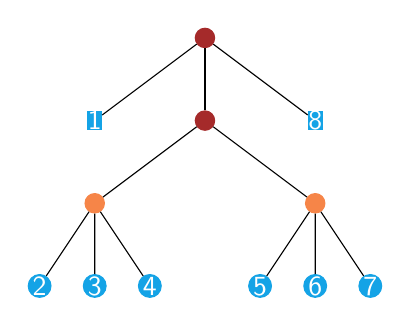
\begin{tikzpicture} [scale = 0.7,level 1/.style = {sibling distance = 2cm, level distance = 1.5cm},					  
		level 2/.style = {sibling distance = 4cm, level distance = 1.5cm},
		level 3/.style = {sibling distance = 1cm, level distance = 1.5cm}]
		\node [deep] {}
		 child{node [digit] {1} 	
		      }
		 child{node [deep] {}
		 		child{node [node] {}
		 				child{node [leaf] {2}}
		 				child{node [leaf] {3}}
		 				child{node [leaf] {4}}
		 			}
			 	child{node [node] {}
		 				child{node [leaf] {5}} 
		 				child{node [leaf] {6}}
		 				child{node [leaf] {7}}
		 			}
		 	 } 
		 child{node [digit] {8}	
		      };
	\end{tikzpicture}
}
\qquad
\subfloat[After ViewL]
{
	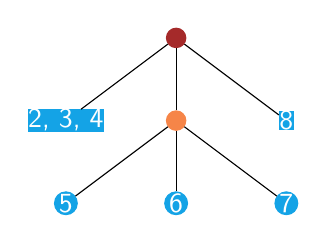
\begin{tikzpicture} [scale = 0.7,level 1/.style = {sibling distance = 2cm, level distance = 1.5cm},					  
		level 2/.style = {sibling distance = 2cm, level distance = 1.5cm},
		level 3/.style = {sibling distance = 2cm, level distance = 1.5cm}]
		\node [deep] {}
		 child{node [digit] {2, 3, 4} 	
		      }
		 child{node [node] {}
				child {node [leaf] {5}}
				child {node [leaf] {6}}
				child {node [leaf] {7}}
		}
		 child{node [digit] {8}	
		      };
	\end{tikzpicture}
}

	\caption{ViewL operation (only including the tails)}
	\label{fig:ftex4}
\end{figure}

Unfortunately, the composition of \AgdaFunction{\_◁\_}(cons) and \AgdaFunction{viewL} is not a no-op, but they both preserve the order of the elements.

\begin{code}
\\
\>\AgdaKeyword{mutual}\<%
\\
%
\\
\>[0]\AgdaIndent{2}{}\<[2]%
\>[2]\AgdaFunction{viewL} \AgdaSymbol{:} \AgdaSymbol{∀} \AgdaSymbol{\{}\AgdaBound{a}\AgdaSymbol{\}} \AgdaSymbol{\{}\AgdaBound{A} \AgdaSymbol{:} \AgdaPrimitiveType{Set} \AgdaBound{a}\AgdaSymbol{\}\{}\AgdaBound{V} \AgdaSymbol{:} \AgdaPrimitiveType{Set} \AgdaBound{a} \AgdaSymbol{\}}\<%
\\
\>[2]\AgdaIndent{10}{}\<[10]%
\>[10]\AgdaSymbol{⦃} \AgdaBound{mo} \AgdaSymbol{:} \AgdaRecord{Monoid} \AgdaBound{V} \AgdaSymbol{⦄}\<%
\\
\>[2]\AgdaIndent{10}{}\<[10]%
\>[10]\AgdaSymbol{⦃} \AgdaBound{m} \AgdaSymbol{:} \AgdaRecord{Measured} \AgdaBound{A} \AgdaBound{V} \AgdaSymbol{⦄}\<%
\\
\>[2]\AgdaIndent{10}{}\<[10]%
\>[10]\AgdaSymbol{\{}\AgdaBound{i} \AgdaSymbol{:} \AgdaBound{V}\AgdaSymbol{\}} \AgdaSymbol{→} \AgdaDatatype{FingerTree} \AgdaBound{A} \AgdaBound{V} \AgdaSymbol{\{}\AgdaBound{i}\AgdaSymbol{\}}\<%
\\
\>[2]\AgdaIndent{10}{}\<[10]%
\>[10]\AgdaSymbol{→} \AgdaDatatype{ViewL} \AgdaBound{A} \AgdaBound{V} \AgdaSymbol{\{}\AgdaBound{i}\AgdaSymbol{\}}\<%
\\
\>[0]\AgdaIndent{2}{}\<[2]%
\>[2]\AgdaFunction{viewL} \AgdaInductiveConstructor{Empty} \AgdaSymbol{=} \AgdaInductiveConstructor{NilL}\<%
\\
\>[0]\AgdaIndent{2}{}\<[2]%
\>[2]\AgdaFunction{viewL} \AgdaSymbol{⦃} \AgdaBound{mo} \AgdaSymbol{⦄} \AgdaSymbol{⦃} \AgdaBound{m} \AgdaSymbol{⦄} \AgdaSymbol{(}\AgdaInductiveConstructor{Single} \AgdaBound{x}\AgdaSymbol{)}\<%
\\
\>[2]\AgdaIndent{4}{}\<[4]%
\>[4]\AgdaKeyword{rewrite} \AgdaFunction{sym} \AgdaSymbol{(}\AgdaField{Monoid.ε-right} \AgdaBound{mo} \AgdaField{∥} \AgdaBound{x} \AgdaField{∥}\AgdaSymbol{)}\<%
\\
\>[2]\AgdaIndent{4}{}\<[4]%
\>[4]\AgdaSymbol{=} \AgdaInductiveConstructor{ConsL} \AgdaBound{x} \AgdaInductiveConstructor{Empty}\<%
\\
\>[0]\AgdaIndent{2}{}\<[2]%
\>[2]\AgdaFunction{viewL} \AgdaSymbol{⦃} \AgdaBound{mo} \AgdaSymbol{⦄} \AgdaSymbol{⦃} \AgdaBound{m} \AgdaSymbol{⦄} \AgdaSymbol{(}\AgdaInductiveConstructor{Deep} \AgdaBound{pr} \AgdaBound{ft} \AgdaBound{sf}\AgdaSymbol{)}\<%
\\
\>[2]\AgdaIndent{4}{}\<[4]%
\>[4]\AgdaKeyword{rewrite} \AgdaFunction{measure-digit-lemma1} \AgdaSymbol{⦃} \AgdaBound{mo} \AgdaSymbol{⦄} \AgdaSymbol{⦃} \AgdaBound{m} \AgdaSymbol{⦄} \AgdaBound{pr} \AgdaBound{ft} \AgdaBound{sf}\<%
\\
\>[2]\AgdaIndent{4}{}\<[4]%
\>[4]\AgdaSymbol{=} \AgdaInductiveConstructor{ConsL} \AgdaSymbol{(}\AgdaFunction{head-dig} \AgdaBound{pr}\AgdaSymbol{)} \AgdaSymbol{(}\AgdaFunction{deepL} \AgdaSymbol{(}\AgdaFunction{tails-dig} \AgdaBound{pr}\AgdaSymbol{)} \AgdaBound{ft} \AgdaBound{sf}\AgdaSymbol{)}\<%
\end{code} \\
\begin{code}
\\
\>[0]\AgdaIndent{2}{}\<[2]%
\>[2]\AgdaFunction{deepL} \AgdaSymbol{:} \AgdaSymbol{∀} \AgdaSymbol{\{}\AgdaBound{a}\AgdaSymbol{\}\{}\AgdaBound{A} \AgdaSymbol{:} \AgdaPrimitiveType{Set} \AgdaBound{a}\AgdaSymbol{\}\{}\AgdaBound{V} \AgdaSymbol{:} \AgdaPrimitiveType{Set} \AgdaBound{a} \AgdaSymbol{\}}\<%
\\
\>[2]\AgdaIndent{8}{}\<[8]%
\>[8]\AgdaSymbol{⦃} \AgdaBound{mo} \AgdaSymbol{:} \AgdaRecord{Monoid} \AgdaBound{V} \AgdaSymbol{⦄}\<%
\\
\>[2]\AgdaIndent{8}{}\<[8]%
\>[8]\AgdaSymbol{⦃} \AgdaBound{m} \AgdaSymbol{:} \AgdaRecord{Measured} \AgdaBound{A} \AgdaBound{V} \AgdaSymbol{⦄}\<%
\\
\>[2]\AgdaIndent{8}{}\<[8]%
\>[8]\AgdaSymbol{\{}\AgdaBound{s} \AgdaSymbol{:} \AgdaBound{V}\AgdaSymbol{\}}\<%
\\
\>[2]\AgdaIndent{8}{}\<[8]%
\>[8]\AgdaSymbol{→} \AgdaSymbol{(}\AgdaBound{pr} \AgdaSymbol{:} \AgdaDatatype{Maybe} \AgdaSymbol{(}\AgdaDatatype{Digit} \AgdaBound{A}\AgdaSymbol{))}\<%
\\
\>[2]\AgdaIndent{8}{}\<[8]%
\>[8]\AgdaSymbol{→} \AgdaSymbol{(}\AgdaBound{ft} \AgdaSymbol{:} \AgdaDatatype{FingerTree} \AgdaSymbol{(}\AgdaDatatype{Node} \AgdaBound{A} \AgdaBound{V}\AgdaSymbol{)} \AgdaBound{V} \AgdaSymbol{\{}\AgdaBound{s}\AgdaSymbol{\})}\<%
\\
\>[2]\AgdaIndent{8}{}\<[8]%
\>[8]\AgdaSymbol{→} \AgdaSymbol{(}\AgdaBound{sf} \AgdaSymbol{:} \AgdaDatatype{Digit} \AgdaBound{A}\AgdaSymbol{)}\<%
\\
\>[2]\AgdaIndent{8}{}\<[8]%
\>[8]\AgdaSymbol{→} \AgdaDatatype{FingerTree} \AgdaBound{A} \AgdaBound{V} \AgdaSymbol{\{}\AgdaFunction{measure-maybe-digit} \AgdaBound{pr} \AgdaField{∙} \AgdaBound{s} \AgdaField{∙} \AgdaFunction{measure-digit} \AgdaBound{sf}\AgdaSymbol{\}}\<%
\\
\>[0]\AgdaIndent{2}{}\<[2]%
\\
\>[0]\AgdaIndent{2}{}\<[2]%
\>[2]\AgdaFunction{deepL} \AgdaSymbol{(}\AgdaInductiveConstructor{just} \AgdaBound{x}\AgdaSymbol{)} \AgdaBound{ft} \AgdaBound{sf} \AgdaSymbol{=} \AgdaInductiveConstructor{Deep} \AgdaBound{x} \AgdaBound{ft} \AgdaBound{sf}\<%
\\
\>[0]\AgdaIndent{2}{}\<[2]%
\>[2]\AgdaFunction{deepL} \AgdaInductiveConstructor{nothing} \AgdaBound{ft} \AgdaBound{sf} \AgdaKeyword{with} \AgdaFunction{viewL} \AgdaBound{ft}\<%
\\
\>[0]\AgdaIndent{2}{}\<[2]%
\>[2]\AgdaFunction{deepL} \AgdaSymbol{⦃} \AgdaBound{mo} \AgdaSymbol{⦄} \AgdaSymbol{⦃} \AgdaBound{m} \AgdaSymbol{⦄} \AgdaInductiveConstructor{nothing} \AgdaBound{ft} \AgdaBound{sf} \AgdaSymbol{|} \AgdaInductiveConstructor{NilL}\<%
\\
\>[2]\AgdaIndent{4}{}\<[4]%
\>[4]\AgdaKeyword{rewrite} \AgdaSymbol{(}\AgdaField{Monoid.ε-left} \AgdaBound{mo}\AgdaSymbol{)} \AgdaSymbol{(}\AgdaField{ε} \AgdaField{∙} \AgdaFunction{measure-digit} \AgdaBound{sf}\AgdaSymbol{)}\<%
\\
\>[4]\AgdaIndent{10}{}\<[10]%
\>[10]\AgdaSymbol{|} \AgdaSymbol{(}\AgdaField{Monoid.ε-left} \AgdaBound{mo}\AgdaSymbol{)} \AgdaSymbol{(}\AgdaFunction{measure-digit} \AgdaBound{sf}\AgdaSymbol{)}\<%
\\
\>[0]\AgdaIndent{4}{}\<[4]%
\>[4]\AgdaSymbol{=} \AgdaFunction{toTree-dig} \AgdaBound{sf}\<%
\\
\>[0]\AgdaIndent{2}{}\<[2]%
\>[2]\AgdaFunction{deepL} \AgdaInductiveConstructor{nothing} \AgdaBound{ft} \AgdaBound{sf} \AgdaSymbol{|} \AgdaInductiveConstructor{ConsL} \AgdaSymbol{(}\AgdaInductiveConstructor{Node2} \AgdaBound{x} \AgdaBound{x₁} \AgdaBound{x₂} \AgdaBound{r}\AgdaSymbol{)} \AgdaBound{x₃}\<%
\\
\>[2]\AgdaIndent{4}{}\<[4]%
\>[4]\AgdaKeyword{rewrite} \AgdaBound{r}\<%
\\
\>[4]\AgdaIndent{10}{}\<[10]%
\>[10]\AgdaSymbol{|} \AgdaFunction{assoc-lemma3} \AgdaBound{x₁} \AgdaBound{x₂} \AgdaSymbol{(}\AgdaFunction{measure-tree} \AgdaBound{x₃}\AgdaSymbol{)} \AgdaBound{sf}\<%
\\
\>[0]\AgdaIndent{4}{}\<[4]%
\>[4]\AgdaSymbol{=} \AgdaInductiveConstructor{Deep} \AgdaSymbol{(}\AgdaInductiveConstructor{Two} \AgdaBound{x₁} \AgdaBound{x₂}\AgdaSymbol{)} \AgdaBound{x₃} \AgdaBound{sf} \AgdaComment{-- Deep (Two x₁ x₂) x₃ sf}\<%
\\
\>[0]\AgdaIndent{2}{}\<[2]%
\>[2]\AgdaFunction{deepL} \AgdaInductiveConstructor{nothing} \AgdaBound{ft} \AgdaBound{sf} \AgdaSymbol{|} \AgdaInductiveConstructor{ConsL} \AgdaSymbol{(}\AgdaInductiveConstructor{Node3} \AgdaBound{x} \AgdaBound{x₁} \AgdaBound{x₂} \AgdaBound{x₃} \AgdaBound{r}\AgdaSymbol{)} \AgdaBound{x₄}\<%
\\
\>[2]\AgdaIndent{4}{}\<[4]%
\>[4]\AgdaKeyword{rewrite} \AgdaBound{r}\<%
\\
\>[4]\AgdaIndent{10}{}\<[10]%
\>[10]\AgdaSymbol{|} \AgdaFunction{assoc-lemma4} \AgdaBound{x₁} \AgdaBound{x₂} \AgdaBound{x₃} \AgdaSymbol{(}\AgdaFunction{measure-tree} \AgdaBound{x₄}\AgdaSymbol{)} \AgdaBound{sf}\<%
\\
\>[0]\AgdaIndent{4}{}\<[4]%
\>[4]\AgdaSymbol{=} \AgdaInductiveConstructor{Deep} \AgdaSymbol{(}\AgdaInductiveConstructor{Three} \AgdaBound{x₁} \AgdaBound{x₂} \AgdaBound{x₃}\AgdaSymbol{)} \AgdaBound{x₄} \AgdaBound{sf} \AgdaComment{-- Deep (Three x₁ x₂ x₃) x₄ sf}\<%
\\
\end{code}

The previous listing represents a pair of mutual recursive functions. \AgdaFunction{deepL} is a variant of the \AgdaInductiveConstructor{Deep} constructor, which also allows the construction of a FingerTree in the case when the first \AgdaDatatype{Digit} is empty (encoded by \AgdaInductiveConstructor{nothing}). The proof that the result has measure "\AgdaFunction{measure-maybe-digit} \AgdaBound{pr} \AgdaField{∙} \AgdaBound{s} \AgdaField{∙} \AgdaFunction{measure-digit} \AgdaBound{sf}" could only be obtained because of the dependently typed implementation of Node. A non-dependently typed version would have required postulating correctness of the Node constructors. 


\subsection{\textit{ViewL} using \textit{Sized Types}}
\label{sec:viewLsize}
An alternative definition of the FingerTree can be indexed by \textit{Size}, as explained in Section \ref{sec:sizedtypes}. In order to simplify things in the following, we are no longer concerned with the correctness of the measurement function, discarding it completely. We only analyse termination checking.

\begin{code}
\\
\>\AgdaKeyword{data} \AgdaDatatype{FingerTree} \AgdaSymbol{\{}\AgdaBound{a} \AgdaSymbol{:} \AgdaPostulate{Level}\AgdaSymbol{\}} \AgdaSymbol{(}\AgdaBound{A} \AgdaSymbol{:} \AgdaPrimitiveType{Set} \AgdaBound{a}\AgdaSymbol{)} \AgdaSymbol{:} \AgdaSymbol{\{}\AgdaBound{size} \AgdaSymbol{:} \AgdaPostulate{Size}\AgdaSymbol{\}} \AgdaSymbol{→} \AgdaPrimitiveType{Set} \AgdaBound{a} \AgdaKeyword{where}\<%
\\
\>[0]\AgdaIndent{2}{}\<[2]%
\>[2]\AgdaInductiveConstructor{Empty} \<[9]%
\>[9]\AgdaSymbol{:} \AgdaSymbol{\{}\AgdaBound{i} \AgdaSymbol{:} \AgdaPostulate{Size}\AgdaSymbol{\}} \AgdaSymbol{→} \AgdaDatatype{FingerTree} \AgdaBound{A} \AgdaSymbol{\{}\AgdaPostulate{↑} \AgdaBound{i}\AgdaSymbol{\}}\<%
\\
\>[0]\AgdaIndent{2}{}\<[2]%
\>[2]\AgdaInductiveConstructor{Single} \AgdaSymbol{:} \AgdaSymbol{\{}\AgdaBound{i} \AgdaSymbol{:} \AgdaPostulate{Size}\AgdaSymbol{\}} \AgdaSymbol{→} \AgdaBound{A} \AgdaSymbol{→} \AgdaDatatype{FingerTree} \AgdaBound{A} \AgdaSymbol{\{}\AgdaPostulate{↑} \AgdaBound{i}\AgdaSymbol{\}}\<%
\\
\>[0]\AgdaIndent{2}{}\<[2]%
\>[2]\AgdaInductiveConstructor{Deep} \<[9]%
\>[9]\AgdaSymbol{:} \AgdaSymbol{\{}\AgdaBound{i} \AgdaSymbol{:} \AgdaPostulate{Size}\AgdaSymbol{\}} \AgdaSymbol{→} \AgdaDatatype{Digit} \AgdaBound{A} \AgdaSymbol{→} \AgdaDatatype{FingerTree} \AgdaSymbol{(}\AgdaDatatype{Node} \AgdaBound{A}\AgdaSymbol{)} \AgdaSymbol{\{}\AgdaBound{i}\AgdaSymbol{\}} \AgdaSymbol{→} \AgdaDatatype{Digit} \AgdaBound{A} \AgdaSymbol{→}\<%
\\
\>[2]\AgdaIndent{11}{}\<[11]%
\>[11]\AgdaDatatype{FingerTree} \AgdaBound{A} \AgdaSymbol{\{}\AgdaPostulate{↑} \AgdaBound{i}\AgdaSymbol{\}}\<%
\\
\end{code} 

This implementation is analogous to the one presented in Section \ref{sec:ftdecl}, after being stripped of all the components related to the measurement.  

The implementation of \AgdaFunction{viewL} illustrates the difficulty of sizing the FingerTrees using Agda's inbuilt sizes \cite{sizedtypes}, as above.

Although the \AgdaFunction{\_◁\_}(cons) operation type-checks,\footnote{I believe that this signals another issue, as after performing a very similar implementation in Appendix \ref{app:termcheck}, I was expecting a failure in the trivial cases. There is more work to be done in this area.} 

\begin{code}
\\
\>\AgdaFunction{\_◁\_} \AgdaSymbol{:} \AgdaSymbol{∀} \AgdaSymbol{\{}\AgdaBound{i} \AgdaBound{a}\AgdaSymbol{\}} \AgdaSymbol{\{}\AgdaBound{A} \AgdaSymbol{:} \AgdaPrimitiveType{Set} \AgdaBound{a}\AgdaSymbol{\}} \AgdaSymbol{→} \AgdaBound{A} \AgdaSymbol{→} \AgdaDatatype{FingerTree} \AgdaBound{A} \AgdaSymbol{\{}\AgdaBound{i}\AgdaSymbol{\}} \AgdaSymbol{→} \AgdaDatatype{FingerTree} \AgdaBound{A} \AgdaSymbol{\{}\AgdaPostulate{↑} \AgdaBound{i}\AgdaSymbol{\}}\<%
\\
\end{code}

implementing the \textit{view} operation is not straightforward. Declaring the analogous data structure (below) stops the implementation of the \AgdaFunction{viewL} method.  

\begin{code}
\\
\>\AgdaKeyword{data} \AgdaDatatype{ViewL} \AgdaSymbol{\{}\AgdaBound{a}\AgdaSymbol{\}(}\AgdaBound{A} \AgdaSymbol{:} \AgdaPrimitiveType{Set} \AgdaBound{a}\AgdaSymbol{)} \AgdaSymbol{:} \AgdaSymbol{\{}\AgdaBound{i} \AgdaSymbol{:} \AgdaPostulate{Size}\AgdaSymbol{\}} \AgdaSymbol{→} \AgdaPrimitiveType{Set} \AgdaBound{a} \AgdaKeyword{where}\<%
\\
\>[0]\AgdaIndent{2}{}\<[2]%
\>[2]\AgdaInductiveConstructor{nilL} \AgdaSymbol{:} \AgdaSymbol{∀} \AgdaSymbol{\{}\AgdaBound{i}\AgdaSymbol{\}} \AgdaSymbol{→} \AgdaDatatype{ViewL} \AgdaBound{A} \AgdaSymbol{\{}\AgdaPostulate{↑} \AgdaBound{i}\AgdaSymbol{\}}\<%
\\
\>[0]\AgdaIndent{2}{}\<[2]%
\>[2]\AgdaInductiveConstructor{consL} \AgdaSymbol{:} \AgdaSymbol{∀} \AgdaSymbol{\{}\AgdaBound{i}\AgdaSymbol{\}} \AgdaSymbol{→} \AgdaBound{A} \AgdaSymbol{→} \AgdaDatatype{FingerTree} \AgdaBound{A} \AgdaSymbol{\{}\AgdaBound{i}\AgdaSymbol{\}} \AgdaSymbol{→} \AgdaDatatype{ViewL} \AgdaBound{A} \AgdaSymbol{\{}\AgdaPostulate{↑} \AgdaBound{i}\AgdaSymbol{\}}\<%
\\
\end{code}

\begin{code}
\\
\>[0]\AgdaIndent{2}{}\<[2]%
\>[2]\AgdaFunction{viewL} \AgdaSymbol{:} \AgdaSymbol{∀} \AgdaSymbol{\{}\AgdaBound{i} \AgdaSymbol{:} \AgdaPostulate{Size}\AgdaSymbol{\}} \AgdaSymbol{\{}\AgdaBound{a}\AgdaSymbol{\}} \AgdaSymbol{\{}\AgdaBound{A} \AgdaSymbol{:} \AgdaPrimitiveType{Set} \AgdaBound{a}\AgdaSymbol{\}} \AgdaSymbol{→} \AgdaDatatype{FingerTree} \AgdaBound{A} \AgdaSymbol{\{}\AgdaBound{i}\AgdaSymbol{\}} \AgdaSymbol{→} \AgdaDatatype{ViewL} \AgdaSymbol{\{}\AgdaBound{a}\AgdaSymbol{\}} \AgdaBound{A} \AgdaSymbol{\{}\AgdaBound{i}\AgdaSymbol{\}}\<%
\\
\>[0]\AgdaIndent{2}{}\<[2]%
\>[2]\AgdaFunction{viewL} \AgdaInductiveConstructor{Empty} \AgdaSymbol{=} \AgdaInductiveConstructor{nilL}\<%
\\
\>[0]\AgdaIndent{2}{}\<[2]%
\>[2]\AgdaFunction{viewL} \AgdaSymbol{(}\AgdaInductiveConstructor{Single} \AgdaBound{x}\AgdaSymbol{)} \AgdaSymbol{=} \AgdaInductiveConstructor{consL} \AgdaBound{x} \AgdaSymbol{\{!  !\}} \AgdaComment{-- consL x (Empty)}\<%
\\
\>[0]\AgdaIndent{2}{}\<[2]%
\>[2]\AgdaFunction{viewL} \AgdaSymbol{(}\AgdaInductiveConstructor{Deep} \AgdaBound{pr} \AgdaBound{m} \AgdaBound{sf}\AgdaSymbol{)} \AgdaSymbol{=} \AgdaSymbol{\{!   !\}} \AgdaComment{-- consL (head pr) (deepL (tail pr) m sf)}\<%
\\
\end{code} 

Two cases are left unsolved. The second one is due to the observation that with \textit{Sized types}, we can only specify a preorder between the argument and the outputs. There is no way to relate the outputs of polymorphic functions in a meaningful way. In this case, we would not be able to decide if \textit{cons}ing an element of type \textit{A} yields a smaller tree than \textit{cons}ing an element of type \AgdaFunction{Node} \textit{A}, which should hold in this case. The error thrown in this case is related to the presence of a negative cycle in the sizing graph. A more detailed example of this issue is in Appendix \ref{app:termcheck}. 
The first issue, however, is because of a design choice in the definition of \textit{Sized Types} that forbids pattern matching\cite{sizedtypes}.

The difficulty of satisfying the termination checker using \textit{Sized Types} is a real bottleneck in Agda programming and should be studied further.

In the next sections, I will continue the implementation of the FingerTree as presented initially, reintroducing the measurement and the indexing.

\subsection{Proving Correctness of \AgdaFunction{viewL}}

We can proceed in an analogous way to the correctness of \AgdaFunction{\_◁\_}(cons) by constructing an appropriate to-list conversion for views, and then proving that the list representations coincide.

However, we stumble upon a simple property that appears difficult to prove in a dependently typed setting. The following issue also occurs in the Coq implementation \cite{coq}, but appears trivial in the Isabelle implementation \cite{isabelle}.

We would like to prove that $viewL(ft)\equiv NilL \iff ft \equiv Empty$. This fact is obvious given the associated definitions. Unfortunately, \textit{Propositional Equality} cannot allow a term of this form, since for an arbitrary $\sigma \in V$, \textit{FingerTree A V} \{$\sigma$\} does not have the same type as Empty. (i.e. \textit{FingerTree A V} \{$\epsilon$\})

Changing the statement of the problem to $\forall$ \textit{ft : FingerTree A V} \{$\epsilon$\} $viewL(ft) \equiv NilL \iff ft \equiv Empty$ allows the definition. However, the type-checker gets stuck trying to case split \textit{ft}. The reason is that it cannot find terms in \textit{V} to satisfy the constrained indexing (e.g. a Deep constructor returning a FingerTree A V \{$\epsilon$\}).

Indeed, if we try to prove this statement on a simpler version of \textit{FingerTree} that is indexed by Size \footnote{so that Empty can assume any size as long as it is smaller than its FingerTree derivatives (such as Deep sf Empty pr)}, it is a straightforward exercise: 

\begin{code}
\\
\>\AgdaFunction{view-lemma3} \AgdaSymbol{:} \AgdaSymbol{∀} \AgdaSymbol{\{}\AgdaBound{a}\AgdaSymbol{\}\{}\AgdaBound{A} \AgdaSymbol{:} \AgdaPrimitiveType{Set} \AgdaBound{a}\AgdaSymbol{\}} \AgdaSymbol{\{}\AgdaBound{V} \AgdaSymbol{:} \AgdaPrimitiveType{Set} \AgdaBound{a} \AgdaSymbol{\}}\<%
\\
\>[2]\AgdaIndent{14}{}\<[14]%
\>[14]\AgdaSymbol{⦃} \AgdaBound{mo} \AgdaSymbol{:} \AgdaRecord{Monoid} \AgdaBound{V} \AgdaSymbol{⦄}\<%
\\
\>[2]\AgdaIndent{14}{}\<[14]%
\>[14]\AgdaSymbol{⦃} \AgdaBound{m} \AgdaSymbol{:} \AgdaRecord{Measured} \AgdaBound{A} \AgdaBound{V} \AgdaSymbol{⦄}\<%
\\
\>[2]\AgdaIndent{14}{}\<[14]%
\>[14]\AgdaSymbol{→} \AgdaSymbol{(}\AgdaBound{ft} \AgdaSymbol{:} \AgdaDatatype{FingerTree} \AgdaBound{A} \AgdaBound{V}\AgdaSymbol{)}\<%
\\
\>[2]\AgdaIndent{14}{}\<[14]%
\>[14]\AgdaSymbol{→} \AgdaSymbol{(}\AgdaFunction{viewL} \AgdaBound{ft} \AgdaDatatype{≡} \AgdaInductiveConstructor{NilL}\AgdaSymbol{)}\<%
\\
\>[2]\AgdaIndent{14}{}\<[14]%
\>[14]\AgdaSymbol{→} \AgdaSymbol{(}\AgdaBound{ft} \AgdaDatatype{≡} \AgdaInductiveConstructor{Empty}\AgdaSymbol{)}\<%
\\
\>\AgdaFunction{view-lemma3} \AgdaInductiveConstructor{Empty} \AgdaBound{p} \AgdaSymbol{=} \AgdaInductiveConstructor{refl}\<%
\\
\>\AgdaFunction{view-lemma3} \AgdaSymbol{(}\AgdaInductiveConstructor{Single} \AgdaBound{x}\AgdaSymbol{)} \AgdaSymbol{()}\<%
\\
\>\AgdaFunction{view-lemma3} \AgdaSymbol{(}\AgdaInductiveConstructor{Deep} \AgdaBound{x} \AgdaBound{x₁} \AgdaBound{ft} \AgdaBound{x₂}\AgdaSymbol{)} \AgdaSymbol{()}\<%
\\
\end{code}

A solution to this issue was suggested by McKinna\cite{hetero}, using an alternate implemenation of equality -- \textit{Heterogeneous Equality}, which unifies the types at a later stage.

Using heterogeneous equality, we can write the original statement in Agda, as well as pattern-match on the FingerTree. However, some problems related to the \AgdaKeyword{with} construct resurface.

\subsection{\AgdaKeyword{with} and \AgdaKeyword{rewrite}}
\label{sec:with}
The implementation abounds in use of \AgdaKeyword{with} and \AgdaKeyword{rewrite} statements. \AgdaKeyword{with}, introduced in the works of McBride and McKinna \cite{viewleft}, allows pattern matching on intermediate computations. \AgdaKeyword{rewrite}, on the other hand, replaces an expression on the left hand side, by making use of a supplied equality relation.

The use of these statements could not be avoided in the implementation of operators that act on indexed data types. As part of the type checking, Agda has to unify the expected type of the result and the actual type of the result. 

\subparagraph{Example.} Consider the implementation of \AgdaFunction{append} on Vectors, but with a slight difference in terms of the index of the result. We return a vector of size $m + n$ instead of $n + m$. The type-checker cannot prove that  $+$ commutes, since it is not superfluous. This does not type-check.

\begin{code}
\\
\>\AgdaFunction{append} \AgdaSymbol{:} \AgdaSymbol{∀} \AgdaSymbol{\{}\AgdaBound{a} \AgdaBound{n} \AgdaBound{m}\AgdaSymbol{\}} \AgdaSymbol{→} \AgdaSymbol{\{}\AgdaBound{A} \AgdaSymbol{:} \AgdaPrimitiveType{Set} \AgdaBound{a}\AgdaSymbol{\}}\<%
\\
\>[4]\AgdaIndent{6}{}\<[6]%
\>[6]\AgdaSymbol{→} \AgdaDatatype{Vec} \AgdaBound{A} \AgdaBound{n}\<%
\\
\>[4]\AgdaIndent{6}{}\<[6]%
\>[6]\AgdaSymbol{→} \AgdaDatatype{Vec} \AgdaBound{A} \AgdaBound{m}\<%
\\
\>[4]\AgdaIndent{6}{}\<[6]%
\>[6]\AgdaSymbol{→} \AgdaDatatype{Vec} \AgdaBound{A} \AgdaSymbol{(}\AgdaBound{m} \AgdaPrimitive{+} \AgdaBound{n}\AgdaSymbol{)}\<%
\\
\>\AgdaFunction{append} \AgdaInductiveConstructor{[]} \AgdaBound{ys} \AgdaSymbol{=} \AgdaBound{ys}\<%
\\
\>\AgdaFunction{append} \AgdaSymbol{(}\AgdaBound{x} \AgdaInductiveConstructor{∷} \AgdaBound{xs}\AgdaSymbol{)} \AgdaBound{ys} \AgdaSymbol{=} \AgdaBound{x} \AgdaInductiveConstructor{∷} \AgdaFunction{append} \AgdaBound{xs} \AgdaBound{ys}\<%
\\
\end{code}

The same situation arises in the proofs about correctness of the measure semantics. With limited support from Agda's proof searching tools, the programmer has to provide proofs that ensure correct typing. Due to the nature of the \textit{Builtin.Equality} relation, there is no trivial refactoring of the code, as suggested in the documentation. \footnote{http://agda.readthedocs.io/en/latest/language/with-abstraction.html}.


\subparagraph{Discussion about \AgdaKeyword{with}.}There are various issues related to the \AgdaKeyword{with} statement that I have stumbled upon:

\begin{itemize}
\item Computing terms that are hidden behind a \AgdaKeyword{with} statement requires recomputation of the expression present in the \AgdaKeyword{with} clause. In the \textit{FingerTree} case, this occurs because of the \AgdaKeyword{rewrite} statements present throughout the implementation of \AgdaFunction{\_◁\_}(cons), \AgdaFunction{viewL}, \AgdaFunction{deepL} etc. This causes a mild inconvenience by having to reiterate the same \textit{rewrite}s whenever one writes proofs about those definitions.

\item Whenever an argument of a function is hidden behind a \textit{with abstraction}, the definition of that function cannot makes use of further \AgdaKeyword{with} statements containing the abstracted expression of the argument. This is discussed in the documentation: Ill-typed with-abstraction \footnote{https://agda.readthedocs.io/en/v2.5.2/language/with-abstraction.html}.
This is the reason that proving the correctness of \AgdaFunction{ViewL} seemed problematic.

\item The type of terms hidden by \textit{with abstraction} is not available, as the feature of type checking in this conditions has not been implemented.

\item There are cases in which the termination-checker is confused in the presence of \AgdaKeyword{with}.

Consider an example in which I try to append an element at the end of a list, which does not type-check.

\begin{code}
\\
\>\AgdaFunction{snoc} \AgdaSymbol{:} \AgdaSymbol{∀} \AgdaSymbol{\{}\AgdaBound{A}\AgdaSymbol{\}} \AgdaSymbol{→} \AgdaBound{A} \AgdaSymbol{→} \AgdaDatatype{List} \AgdaBound{A} \AgdaSymbol{→} \AgdaDatatype{List} \AgdaBound{A}\<%
\\
\>\AgdaFunction{snoc} \AgdaBound{x} \AgdaBound{xs} \AgdaKeyword{with} \AgdaBound{xs}\<%
\\
\>\AgdaFunction{snoc} \AgdaBound{x} \AgdaBound{xs} \AgdaSymbol{|} \AgdaInductiveConstructor{[]} \AgdaSymbol{=} \AgdaBound{x} \AgdaInductiveConstructor{∷} \AgdaInductiveConstructor{[]}\<%
\\
\>\AgdaFunction{snoc} \AgdaBound{x} \AgdaBound{xs} \AgdaSymbol{|} \AgdaBound{y} \AgdaInductiveConstructor{∷} \AgdaBound{ys} \AgdaSymbol{=} \AgdaBound{y} \AgdaInductiveConstructor{∷} \AgdaSymbol{(}\AgdaFunction{snoc} \AgdaBound{x} \AgdaBound{ys}\AgdaSymbol{)}\<%
\\
\end{code} 

\end{itemize}

Taking these issues into account, I have tried to come up with solutions to some of them. I will present them after finishing the main implementation of the FingerTree.

I should note here that the proofs that I am making are still providing a powerful verification, since the FingerTree maintains all invariants and the measurement semantics is preserved and used sanely.

\subsection{Folding}
\label{sec:fold}

Next, I implement the fold operation and show its correctness. I will only present the fold-left implementation, since fold-right is analogous. \footnote{
To exemplify the semantics of foldl on a list, consider \textit{foldl f s [x, y, z] = f (f (f s x) y) z}.}

Defining folds on \textbf{Node} and \textbf{Digit} is trivial, since they are just length constrained lists. I have presented them in the Appendix. Consider its implementation on the FingerTree: 

\begin{code}
\\
\>\AgdaFunction{foldl} \AgdaSymbol{:} \AgdaSymbol{∀} \AgdaSymbol{\{}\AgdaBound{a}\AgdaSymbol{\}} \AgdaSymbol{\{}\AgdaBound{A} \AgdaSymbol{:} \AgdaPrimitiveType{Set} \AgdaBound{a}\AgdaSymbol{\}} \AgdaSymbol{\{}\AgdaBound{V} \AgdaSymbol{:} \AgdaPrimitiveType{Set} \AgdaBound{a}\AgdaSymbol{\}}\<%
\\
\>[2]\AgdaIndent{8}{}\<[8]%
\>[8]\AgdaSymbol{\{}\AgdaBound{W} \AgdaSymbol{:} \AgdaPrimitiveType{Set} \AgdaBound{a}\AgdaSymbol{\}}\<%
\\
\>[2]\AgdaIndent{8}{}\<[8]%
\>[8]\AgdaSymbol{⦃} \AgdaBound{mo} \AgdaSymbol{:} \AgdaRecord{Monoid} \AgdaBound{V} \AgdaSymbol{⦄}\<%
\\
\>[2]\AgdaIndent{8}{}\<[8]%
\>[8]\AgdaSymbol{⦃} \AgdaBound{m} \AgdaSymbol{:} \AgdaRecord{Measured} \AgdaBound{A} \AgdaBound{V} \AgdaSymbol{⦄}\<%
\\
\>[2]\AgdaIndent{8}{}\<[8]%
\>[8]\AgdaSymbol{\{}\AgdaBound{s} \AgdaSymbol{:} \AgdaBound{V}\AgdaSymbol{\}}\<%
\\
\>[2]\AgdaIndent{8}{}\<[8]%
\>[8]\AgdaSymbol{→} \AgdaSymbol{(}\AgdaBound{W} \AgdaSymbol{→} \AgdaBound{A} \AgdaSymbol{→} \AgdaBound{W}\AgdaSymbol{)}\<%
\\
\>[2]\AgdaIndent{8}{}\<[8]%
\>[8]\AgdaSymbol{→} \AgdaBound{W}\<%
\\
\>[2]\AgdaIndent{8}{}\<[8]%
\>[8]\AgdaSymbol{→} \AgdaDatatype{FingerTree} \AgdaBound{A} \AgdaBound{V} \AgdaSymbol{\{}\AgdaBound{s}\AgdaSymbol{\}}\<%
\\
\>[2]\AgdaIndent{8}{}\<[8]%
\>[8]\AgdaSymbol{→} \AgdaBound{W}\<%
\\
\>\AgdaFunction{foldl} \AgdaBound{f} \AgdaBound{i} \AgdaInductiveConstructor{Empty} \AgdaSymbol{=} \AgdaBound{i}\<%
\\
\>\AgdaFunction{foldl} \AgdaBound{f} \AgdaBound{i} \AgdaSymbol{(}\AgdaInductiveConstructor{Single} \AgdaBound{e}\AgdaSymbol{)} \AgdaSymbol{=} \AgdaBound{f} \AgdaBound{i} \AgdaBound{e}\<%
\\
\>\AgdaFunction{foldl} \AgdaSymbol{\{}\AgdaArgument{W} \AgdaSymbol{=} \AgdaBound{W}\AgdaSymbol{\}} \AgdaBound{f} \AgdaBound{i} \AgdaSymbol{(}\AgdaInductiveConstructor{Deep} \AgdaBound{pr} \AgdaBound{ft} \AgdaBound{sf}\AgdaSymbol{)} \AgdaSymbol{=}\<%
\\
\>[0]\AgdaIndent{2}{}\<[2]%
\>[2]\AgdaFunction{foldl-dig} \AgdaBound{f} \AgdaSymbol{(}\AgdaFunction{foldl} \AgdaSymbol{(}\AgdaFunction{foldl-node} \AgdaBound{f}\AgdaSymbol{)} \AgdaSymbol{(}\AgdaFunction{foldl-dig} \AgdaBound{f} \AgdaBound{i} \AgdaBound{pr}\AgdaSymbol{)} \AgdaBound{ft}\AgdaSymbol{)} \AgdaBound{sf}\<%
\\
\end{code}

The operation of folding over nested types has been extensively studied \cite{nestedhinze}. Further exemplifying  implementations can be found in .... works \cite{debrujin}.

\subsection{Proving correctness of Fold Left}

Next, I will show that the previous implementation is sane, by seeing whether folding over a FingerTree is equivalent to folding over its list representation.

\begin{code}
\\
\>\AgdaFunction{foldl-correct} \AgdaSymbol{:} \AgdaSymbol{∀} \AgdaSymbol{\{}\AgdaBound{a}\AgdaSymbol{\}} \AgdaSymbol{\{}\AgdaBound{A} \AgdaSymbol{:} \AgdaPrimitiveType{Set} \AgdaBound{a}\AgdaSymbol{\}\{}\AgdaBound{V} \AgdaSymbol{:} \AgdaPrimitiveType{Set} \AgdaBound{a}\AgdaSymbol{\}}\<%
\\
\>[2]\AgdaIndent{14}{}\<[14]%
\>[14]\AgdaSymbol{\{}\AgdaBound{W} \AgdaSymbol{:} \AgdaPrimitiveType{Set} \AgdaBound{a}\AgdaSymbol{\}}\<%
\\
\>[2]\AgdaIndent{14}{}\<[14]%
\>[14]\AgdaSymbol{⦃} \AgdaBound{mo} \AgdaSymbol{:} \AgdaRecord{Monoid} \AgdaBound{V} \AgdaSymbol{⦄}\<%
\\
\>[2]\AgdaIndent{14}{}\<[14]%
\>[14]\AgdaSymbol{⦃} \AgdaBound{m} \AgdaSymbol{:} \AgdaRecord{Measured} \AgdaBound{A} \AgdaBound{V} \AgdaSymbol{⦄}\<%
\\
\>[2]\AgdaIndent{14}{}\<[14]%
\>[14]\AgdaSymbol{→} \AgdaSymbol{\{}\AgdaBound{s} \AgdaSymbol{:} \AgdaBound{V}\AgdaSymbol{\}}\<%
\\
\>[2]\AgdaIndent{14}{}\<[14]%
\>[14]\AgdaSymbol{→} \AgdaSymbol{(}\AgdaBound{f} \AgdaSymbol{:} \AgdaBound{W} \AgdaSymbol{→} \AgdaBound{A} \AgdaSymbol{→} \AgdaBound{W}\AgdaSymbol{)}\<%
\\
\>[2]\AgdaIndent{14}{}\<[14]%
\>[14]\AgdaSymbol{→} \AgdaSymbol{(}\AgdaBound{σ} \AgdaSymbol{:} \AgdaBound{W}\AgdaSymbol{)}\<%
\\
\>[2]\AgdaIndent{14}{}\<[14]%
\>[14]\AgdaSymbol{→} \AgdaSymbol{(}\AgdaBound{ft} \AgdaSymbol{:} \AgdaDatatype{FingerTree} \AgdaBound{A} \AgdaBound{V} \AgdaSymbol{\{}\AgdaBound{s}\AgdaSymbol{\})}\<%
\\
\>[2]\AgdaIndent{14}{}\<[14]%
\>[14]\AgdaSymbol{→} \AgdaSymbol{(}\AgdaFunction{foldl} \AgdaBound{f} \AgdaBound{σ} \AgdaBound{ft} \AgdaDatatype{≡} \AgdaFunction{Data.List.foldl} \AgdaBound{f} \AgdaBound{σ} \AgdaSymbol{(}\AgdaFunction{toList-ft} \AgdaBound{ft}\AgdaSymbol{))}\<%
\\
\end{code}


Furthermore, we can prove that if we fold over the FingerTree using the \textbf{Monoid} and the \textbf{Measure}\footnote{foldfun v x = v $∙ \Vert$ x $\Vert$} over which it is instantiated, we obtain the same result as the measure. 

\begin{code}
\\
\>\AgdaFunction{foldl-lemma0} \AgdaSymbol{:} \AgdaSymbol{∀} \AgdaSymbol{\{}\AgdaBound{a}\AgdaSymbol{\}} \AgdaSymbol{\{}\AgdaBound{A} \AgdaSymbol{:} \AgdaPrimitiveType{Set} \AgdaBound{a}\AgdaSymbol{\}} \AgdaSymbol{\{}\AgdaBound{V} \AgdaSymbol{:} \AgdaPrimitiveType{Set} \AgdaBound{a}\AgdaSymbol{\}}\<%
\\
\>[2]\AgdaIndent{14}{}\<[14]%
\>[14]\AgdaSymbol{⦃} \AgdaBound{mo} \AgdaSymbol{:} \AgdaRecord{Monoid} \AgdaBound{V} \AgdaSymbol{⦄}\<%
\\
\>[2]\AgdaIndent{14}{}\<[14]%
\>[14]\AgdaSymbol{⦃} \AgdaBound{m} \AgdaSymbol{:} \AgdaRecord{Measured} \AgdaBound{A} \AgdaBound{V} \AgdaSymbol{⦄}\<%
\\
\>[2]\AgdaIndent{14}{}\<[14]%
\>[14]\AgdaSymbol{→} \AgdaSymbol{\{}\AgdaBound{s} \AgdaSymbol{:} \AgdaBound{V}\AgdaSymbol{\}}\<%
\\
\>[2]\AgdaIndent{14}{}\<[14]%
\>[14]\AgdaSymbol{→} \AgdaSymbol{(}\AgdaBound{v} \AgdaSymbol{:} \AgdaBound{V}\AgdaSymbol{)}\<%
\\
\>[2]\AgdaIndent{14}{}\<[14]%
\>[14]\AgdaSymbol{→} \AgdaSymbol{(}\AgdaBound{ft} \AgdaSymbol{:} \AgdaDatatype{FingerTree} \AgdaBound{A} \AgdaBound{V} \AgdaSymbol{\{}\AgdaBound{s}\AgdaSymbol{\})}\<%
\\
\>[2]\AgdaIndent{14}{}\<[14]%
\>[14]\AgdaSymbol{→} \AgdaSymbol{(}\AgdaFunction{foldl} \AgdaFunction{foldfun} \AgdaBound{v} \AgdaBound{ft} \AgdaDatatype{≡} \AgdaBound{v} \AgdaField{∙} \AgdaBound{s}\AgdaSymbol{)}\<%
\\
\end{code}

This result is important as a sanity check of the measure semantics we are trying to preserve throughout the implementation, since this fact can only be true if we preserve the order of calls to the monoid operator.

\subsection{Splitting}

Splitting is an extension of the ViewL paradigm, which allows extraction of elements arbitrarily far in the FingerTree. It consists of a left side, a middle element, and a right side.\footnote{the sides are correct FingerTrees}

The same issues occur, as in the case of viewL. I have tried in this implementation to keep the usage of \AgdaKeyword{with} to a minimum. This turned out to be a very difficult task, so correctness of this method can only be provided in terms of its measure, which is being taken care of by the indexing.

The split is done over a boolean predicate, $p \in V \to Bool$ and a starting value, $i \in V$. The method iterates through the FingerTree, element by element, at each step increasing $i$ by the measure of the current element, $\Vert x \Vert$. The split returns when the value of the predicate turns true $p(i) = True$, giving the element at which this change occurs as the middle.


As with ViewL, we create an additional data-type that will represent the result. It is indexed by the measurement, ensuring correctness.

\begin{code}
\\
\>\AgdaKeyword{data} \AgdaDatatype{Split-d} \AgdaSymbol{\{}\AgdaBound{a}\AgdaSymbol{\}} \AgdaSymbol{(}\AgdaBound{A} \AgdaSymbol{:} \AgdaPrimitiveType{Set} \AgdaBound{a}\AgdaSymbol{)} \AgdaSymbol{(}\AgdaBound{V} \AgdaSymbol{:} \AgdaPrimitiveType{Set} \AgdaBound{a}\AgdaSymbol{)}\<%
\\
\>[2]\AgdaIndent{12}{}\<[12]%
\>[12]\AgdaSymbol{⦃} \AgdaBound{mo} \AgdaSymbol{:} \AgdaRecord{Monoid} \AgdaBound{V} \AgdaSymbol{⦄}\<%
\\
\>[2]\AgdaIndent{12}{}\<[12]%
\>[12]\AgdaSymbol{⦃} \AgdaBound{m} \AgdaSymbol{:} \AgdaRecord{Measured} \AgdaBound{A} \AgdaBound{V} \AgdaSymbol{⦄} \AgdaSymbol{:}\<%
\\
\>[2]\AgdaIndent{12}{}\<[12]%
\>[12]\AgdaSymbol{\{}\AgdaBound{μ} \AgdaSymbol{:} \AgdaBound{V}\AgdaSymbol{\}} \AgdaSymbol{→} \AgdaPrimitiveType{Set} \AgdaBound{a} \AgdaKeyword{where}\<%
\\
\>[0]\AgdaIndent{2}{}\<[2]%
\>[2]\AgdaInductiveConstructor{split-d} \AgdaSymbol{:} \AgdaSymbol{∀} \AgdaSymbol{\{}\AgdaBound{μ₁} \AgdaSymbol{:} \AgdaBound{V}\AgdaSymbol{\}} \AgdaSymbol{\{}\AgdaBound{μ₂} \AgdaSymbol{:} \AgdaBound{V}\AgdaSymbol{\}}\<%
\\
\>[2]\AgdaIndent{10}{}\<[10]%
\>[10]\AgdaSymbol{→} \AgdaSymbol{(}\AgdaDatatype{FingerTree} \AgdaBound{A} \AgdaBound{V} \AgdaSymbol{\{}\AgdaBound{μ₁}\AgdaSymbol{\})} \<[35]%
\>[35]\AgdaComment{-- left side}\<%
\\
\>[2]\AgdaIndent{10}{}\<[10]%
\>[10]\AgdaSymbol{→} \AgdaSymbol{(}\AgdaBound{x} \AgdaSymbol{:} \AgdaBound{A}\AgdaSymbol{)} \<[35]%
\>[35]\AgdaComment{-- middle}\<%
\\
\>[2]\AgdaIndent{10}{}\<[10]%
\>[10]\AgdaSymbol{→} \AgdaSymbol{(}\AgdaDatatype{FingerTree} \AgdaBound{A} \AgdaBound{V} \AgdaSymbol{\{}\AgdaBound{μ₂}\AgdaSymbol{\})} \<[35]%
\>[35]\AgdaComment{-- right side}\<%
\\
\>[2]\AgdaIndent{10}{}\<[10]%
\>[10]\AgdaSymbol{→} \AgdaDatatype{Split-d} \AgdaBound{A} \AgdaBound{V} \AgdaSymbol{\{}\AgdaBound{μ₁} \AgdaField{∙} \AgdaField{∥} \AgdaBound{x} \AgdaField{∥} \AgdaField{∙} \AgdaBound{μ₂}\AgdaSymbol{\}}\<%
\\
\end{code}

Since this implementation is long and full of necessary proofs about the types, I will only provide the most important snippets.

\subparagraph{Discussion} This implementation was also made difficult because of the partiality of the function in the original paper. Wrapping things in the Maybe monad can confuse the type-checker at times.

\subparagraph{The main procedure}pattern matches on the constructors for the FingerTree provided as argument. Notice that the typing already maintains the invariant.

\begin{code}
\\
\>[0]\AgdaIndent{2}{}\<[2]%
\>[2]\AgdaFunction{split-Tree} \AgdaSymbol{:} \AgdaSymbol{∀} \AgdaSymbol{\{}\AgdaBound{a}\AgdaSymbol{\}} \AgdaSymbol{\{}\AgdaBound{A} \AgdaSymbol{:} \AgdaPrimitiveType{Set} \AgdaBound{a}\AgdaSymbol{\}} \AgdaSymbol{\{}\AgdaBound{V} \AgdaSymbol{:} \AgdaPrimitiveType{Set} \AgdaBound{a}\AgdaSymbol{\}}\<%
\\
\>[2]\AgdaIndent{14}{}\<[14]%
\>[14]\AgdaSymbol{⦃} \AgdaBound{mo} \AgdaSymbol{:} \AgdaRecord{Monoid} \AgdaBound{V} \AgdaSymbol{⦄}\<%
\\
\>[2]\AgdaIndent{14}{}\<[14]%
\>[14]\AgdaSymbol{⦃} \AgdaBound{m} \AgdaSymbol{:} \AgdaRecord{Measured} \AgdaBound{A} \AgdaBound{V} \AgdaSymbol{⦄}\<%
\\
\>[2]\AgdaIndent{14}{}\<[14]%
\>[14]\AgdaSymbol{\{}\AgdaBound{μ} \AgdaSymbol{:} \AgdaBound{V}\AgdaSymbol{\}} \AgdaComment{-- type class information}\<%
\\
\>[2]\AgdaIndent{14}{}\<[14]%
\>[14]\AgdaSymbol{→} \AgdaSymbol{(}\AgdaBound{p} \AgdaSymbol{:} \AgdaBound{V} \AgdaSymbol{→} \AgdaDatatype{Bool}\AgdaSymbol{)} \AgdaSymbol{→} \AgdaSymbol{(}\AgdaBound{i} \AgdaSymbol{:} \AgdaBound{V}\AgdaSymbol{)} \AgdaComment{-- predicate and initial value}\<%
\\
\>[2]\AgdaIndent{14}{}\<[14]%
\>[14]\AgdaSymbol{→} \AgdaSymbol{(}\AgdaBound{ft} \AgdaSymbol{:} \AgdaDatatype{FingerTree} \AgdaBound{A} \AgdaBound{V} \AgdaSymbol{\{}\AgdaBound{μ}\AgdaSymbol{\})} \AgdaComment{-- argument}\<%
\\
\>[2]\AgdaIndent{14}{}\<[14]%
\>[14]\AgdaSymbol{→} \AgdaDatatype{Maybe} \AgdaSymbol{(}\AgdaDatatype{Split-d} \AgdaBound{A} \AgdaBound{V} \AgdaSymbol{\{}\AgdaBound{μ}\AgdaSymbol{\})}\<%
\\
\>[0]\AgdaIndent{2}{}\<[2]%
\>[2]\AgdaFunction{split-Tree} \AgdaBound{p} \AgdaBound{i} \AgdaInductiveConstructor{Empty}\<%
\\
\>[2]\AgdaIndent{4}{}\<[4]%
\>[4]\AgdaSymbol{=} \AgdaInductiveConstructor{nothing} \<[15]%
\>[15]\AgdaComment{-- cannot split an empty tree}\<%
\\
\>[0]\AgdaIndent{2}{}\<[2]%
\>[2]\AgdaFunction{split-Tree} \AgdaBound{p} \AgdaBound{i} \AgdaSymbol{(}\AgdaInductiveConstructor{Single} \AgdaBound{e}\AgdaSymbol{)}\<%
\\
\>[2]\AgdaIndent{4}{}\<[4]%
\>[4]\AgdaSymbol{=} \AgdaInductiveConstructor{just} \AgdaSymbol{(}\AgdaFunction{split-Tree-single} \AgdaBound{p} \AgdaBound{i} \AgdaBound{e}\AgdaSymbol{)} \AgdaComment{-- superfluous case}\<%
\\
\>[0]\AgdaIndent{2}{}\<[2]%
\>[2]\AgdaFunction{split-Tree} \AgdaBound{p} \AgdaBound{i} \AgdaSymbol{(}\AgdaInductiveConstructor{Deep} \AgdaBound{pr} \AgdaBound{ft} \AgdaBound{sf}\AgdaSymbol{)}\<%
\\
\>[2]\AgdaIndent{4}{}\<[4]%
\>[4]\AgdaSymbol{=} \AgdaInductiveConstructor{just} \AgdaSymbol{(}\AgdaFunction{split-Tree-if} \AgdaBound{p} \AgdaBound{i} \AgdaBound{pr} \AgdaBound{ft} \AgdaBound{sf} \AgdaFunction{vpr} \AgdaInductiveConstructor{refl} \AgdaFunction{vft} \AgdaInductiveConstructor{refl}\AgdaSymbol{)} \AgdaComment{-- recursive case}\<%
\\
\>[2]\AgdaIndent{4}{}\<[4]%
\>[4]\AgdaKeyword{where}\<%
\\
\>[4]\AgdaIndent{6}{}\<[6]%
\>[6]\AgdaFunction{vpr} \AgdaSymbol{=} \AgdaBound{p} \AgdaSymbol{(}\AgdaBound{i} \AgdaField{∙} \AgdaSymbol{(}\AgdaFunction{measure-digit} \AgdaBound{pr}\AgdaSymbol{))}\<%
\\
\>[4]\AgdaIndent{6}{}\<[6]%
\>[6]\AgdaFunction{vft} \AgdaSymbol{=} \AgdaBound{p} \AgdaSymbol{((}\AgdaBound{i} \AgdaField{∙} \AgdaFunction{measure-digit} \AgdaBound{pr}\AgdaSymbol{)} \AgdaField{∙} \AgdaFunction{measure-tree} \AgdaBound{ft}\AgdaSymbol{)}\<%
\\
\end{code}


The \textbf{split-Tree-if} function splits the computation in three cases, depending on where the predicate changes to \textit{True}. This could happen during the prefix \textbf{pr}, during the nested FingerTree \textbf{ft} or during the suffix \textbf{sf}:

\begin{code}
\\
\>[0]\AgdaIndent{2}{}\<[2]%
\>[2]\AgdaFunction{split-Tree-if} \AgdaSymbol{:} \AgdaSymbol{∀} \AgdaSymbol{\{}\AgdaBound{a}\AgdaSymbol{\}} \AgdaSymbol{\{}\AgdaBound{A} \AgdaSymbol{:} \AgdaPrimitiveType{Set} \AgdaBound{a}\AgdaSymbol{\}} \AgdaSymbol{\{}\AgdaBound{V} \AgdaSymbol{:} \AgdaPrimitiveType{Set} \AgdaBound{a}\AgdaSymbol{\}}\<%
\\
\>[2]\AgdaIndent{16}{}\<[16]%
\>[16]\AgdaSymbol{⦃} \AgdaBound{mo} \AgdaSymbol{:} \AgdaRecord{Monoid} \AgdaBound{V} \AgdaSymbol{⦄}\<%
\\
\>[2]\AgdaIndent{16}{}\<[16]%
\>[16]\AgdaSymbol{⦃} \AgdaBound{m} \AgdaSymbol{:} \AgdaRecord{Measured} \AgdaBound{A} \AgdaBound{V} \AgdaSymbol{⦄}\<%
\\
\>[2]\AgdaIndent{16}{}\<[16]%
\>[16]\AgdaSymbol{\{}\AgdaBound{μ} \AgdaSymbol{:} \AgdaBound{V}\AgdaSymbol{\}}\<%
\\
\>[2]\AgdaIndent{16}{}\<[16]%
\>[16]\AgdaSymbol{→} \AgdaSymbol{(}\AgdaBound{p} \AgdaSymbol{:} \AgdaBound{V} \AgdaSymbol{→} \AgdaDatatype{Bool}\AgdaSymbol{)} \AgdaSymbol{→} \AgdaSymbol{(}\AgdaBound{i} \AgdaSymbol{:} \AgdaBound{V}\AgdaSymbol{)} \<[44]%
\>[44]\AgdaComment{-- predicate and initial value}\<%
\\
\>[2]\AgdaIndent{16}{}\<[16]%
\>[16]\AgdaSymbol{→} \AgdaSymbol{(}\AgdaBound{pr} \AgdaSymbol{:} \AgdaDatatype{Digit} \AgdaBound{A}\AgdaSymbol{)} \<[45]%
\>[45]\AgdaComment{-- prefix}\<%
\\
\>[2]\AgdaIndent{16}{}\<[16]%
\>[16]\AgdaSymbol{→} \AgdaSymbol{(}\AgdaBound{ft} \AgdaSymbol{:} \AgdaDatatype{FingerTree} \AgdaSymbol{(}\AgdaDatatype{Node} \AgdaBound{A} \AgdaBound{V}\AgdaSymbol{)} \AgdaBound{V} \AgdaSymbol{\{}\AgdaBound{μ}\AgdaSymbol{\})} \AgdaComment{-- nested tree}\<%
\\
\>[2]\AgdaIndent{16}{}\<[16]%
\>[16]\AgdaSymbol{→} \AgdaSymbol{(}\AgdaBound{sf} \AgdaSymbol{:} \AgdaDatatype{Digit} \AgdaBound{A}\AgdaSymbol{)} \<[43]%
\>[43]\AgdaComment{-- suffix}\<%
\\
\>[2]\AgdaIndent{16}{}\<[16]%
\>[16]\AgdaSymbol{→} \AgdaSymbol{(}\AgdaBound{vpr} \AgdaSymbol{:} \AgdaDatatype{Bool}\AgdaSymbol{)} \<[43]%
\>[43]\AgdaComment{-- value of predicate after prefix}\<%
\\
\>[2]\AgdaIndent{16}{}\<[16]%
\>[16]\AgdaSymbol{→} \AgdaSymbol{(}\AgdaBound{vpr} \AgdaDatatype{≡} \AgdaBound{p} \AgdaSymbol{(}\AgdaBound{i} \AgdaField{∙} \AgdaFunction{measure-digit} \AgdaBound{pr}\AgdaSymbol{))} \AgdaComment{-- correctness check}\<%
\\
\>[2]\AgdaIndent{16}{}\<[16]%
\>[16]\AgdaSymbol{→} \AgdaSymbol{(}\AgdaBound{vft} \AgdaSymbol{:} \AgdaDatatype{Bool}\AgdaSymbol{)} \<[43]%
\>[43]\AgdaComment{-- value of predicate after tree}\<%
\\
\>[2]\AgdaIndent{16}{}\<[16]%
\>[16]\AgdaSymbol{→} \AgdaSymbol{(}\AgdaBound{vft} \AgdaDatatype{≡} \AgdaBound{p} \AgdaSymbol{((}\AgdaBound{i} \AgdaField{∙} \AgdaFunction{measure-digit} \AgdaBound{pr}\AgdaSymbol{)} \AgdaField{∙} \AgdaSymbol{(}\AgdaFunction{measure-tree} \AgdaBound{ft}\AgdaSymbol{)))} \AgdaComment{-- check}\<%
\\
\>[2]\AgdaIndent{16}{}\<[16]%
\>[16]\AgdaSymbol{→} \AgdaDatatype{Split-d} \AgdaBound{A} \AgdaBound{V} \AgdaSymbol{\{(}\AgdaFunction{measure-digit} \AgdaBound{pr}\AgdaSymbol{)} \AgdaField{∙} \AgdaBound{μ} \AgdaField{∙} \AgdaSymbol{(}\AgdaFunction{measure-digit} \AgdaBound{sf}\AgdaSymbol{)\}}\<%
\\
\>[0]\AgdaIndent{2}{}\<[2]%
\>[2]\AgdaFunction{split-Tree-if} \AgdaBound{p} \AgdaBound{i} \AgdaBound{pr} \AgdaBound{ft} \AgdaBound{sf} \AgdaInductiveConstructor{false} \AgdaBound{pr1} \AgdaInductiveConstructor{false} \AgdaBound{pr2}\<%
\\
\>[2]\AgdaIndent{4}{}\<[4]%
\>[4]\AgdaSymbol{=} \AgdaFunction{split-Tree2} \AgdaBound{p} \AgdaSymbol{((}\AgdaBound{i} \AgdaField{∙} \AgdaFunction{measure-digit} \AgdaBound{pr}\AgdaSymbol{)} \AgdaField{∙} \AgdaSymbol{(}\AgdaFunction{measure-tree} \AgdaBound{ft}\AgdaSymbol{))} \AgdaBound{pr} \AgdaBound{ft} \AgdaBound{sf}\<%
\\
\>[2]\AgdaIndent{4}{}\<[4]%
\>[4]\AgdaComment{-- case2 : predicate becomes true in suffix or not at all}\<%
\\
\>[0]\AgdaIndent{2}{}\<[2]%
\>[2]\AgdaFunction{split-Tree-if} \AgdaBound{p} \AgdaBound{i} \AgdaBound{pr} \AgdaBound{ft} \AgdaBound{sf} \AgdaInductiveConstructor{false} \AgdaBound{pr1} \AgdaInductiveConstructor{true} \AgdaBound{pr2}\<%
\\
\>[2]\AgdaIndent{4}{}\<[4]%
\>[4]\AgdaSymbol{=} \AgdaFunction{split-Tree3} \AgdaBound{p} \AgdaBound{i} \AgdaBound{pr} \AgdaBound{ft} \AgdaBound{sf} \AgdaSymbol{(}\AgdaFunction{sym} \AgdaBound{pr1}\AgdaSymbol{)} \AgdaSymbol{(}\AgdaFunction{sym} \AgdaBound{pr2}\AgdaSymbol{)}\<%
\\
\>[2]\AgdaIndent{4}{}\<[4]%
\>[4]\AgdaComment{-- case3 : predicate becomes true in tree}\<%
\\
\>[0]\AgdaIndent{2}{}\<[2]%
\>[2]\AgdaFunction{split-Tree-if} \AgdaBound{p} \AgdaBound{i} \AgdaBound{pr} \AgdaBound{ft} \AgdaBound{sf} \AgdaInductiveConstructor{true} \AgdaBound{pr1} \AgdaBound{vft} \AgdaBound{pr2}\<%
\\
\>[2]\AgdaIndent{4}{}\<[4]%
\>[4]\AgdaSymbol{=} \AgdaFunction{split-Tree1} \AgdaBound{p} \AgdaBound{i} \AgdaBound{pr} \AgdaBound{ft} \AgdaBound{sf}\<%
\\
\>[2]\AgdaIndent{4}{}\<[4]%
\>[4]\AgdaComment{-- case1 : predicate becomes true in prefix}\<%
\\
\end{code}

The full implementation requires more advanced Agda syntax, as well as the implementation of the ViewR and deepR. I will provide an explanation of why this application was more difficult in section \ref{eval:lemma}.

\section{Proving correctness}

As in the case with viewL, proving statements about results with of a split application requires type checking within with abstractions. This feature is not available yet in Agda (throws the error: "Feature not Implemented") and I could not find a way around it.

However, as suggested in \cite{coq}, the aim of the proof, namely that: For all ft, left, right : FingerTree, p : Boolean predicate, i : value and m : element of the finger tree, it must be the case that: \\
\indent\indent	if \AgdaFunction{split} \textit{p} \textit{i} \textit{ft} = \AgdaInductiveConstructor{split-d} \textit{left m right} \\ 
\indent\indent 	then \AgdaFunction{toList-ft} \textit{ft}    = (\AgdaFunction{toList-ft} \textit{left}) ++ [ \textit{m} ] ++ (\AgdaFunction{toList-ft} \textit{right})\\
However, the type signature of the split function already ensures that:\\ 
\indent\indent $\Vert$ \textit{ft} $\Vert$ = $\Vert$\AgdaFunction{split} \textit{p} \textit{i}  \textit{ft} $\Vert$\\
For the specific instance of the FingerTree using an arbitrary type \textit{A} for elements and having values of type \textit{A} 	\AgdaFunction{List}: \\
\indent\indent ft : \AgdaFunction{FingerTree} \textit{A} (\textit{A} \AgdaFunction{List}) \\
instantiated with the measurement which turns elements to singleton lists and the list monoid \footnote{nil is the neuter element, and list concatenation (++) is an associative operation}, we would find that: \\
\indent\indent $\Vert$ \textit{ft} $\Vert$ = \AgdaFunction{foldl-ft} \AgdaFunction{\_++\_} \AgdaInductiveConstructor{[]} \textit{ft} = \AgdaFunction{toList-ft} \textit{ft} \\
Given the fact that the size of split is given by \AgdaBound{μ₁} \AgdaField{∙} \AgdaField{∥} \AgdaBound{x} \AgdaField{∥} \AgdaField{∙} \AgdaBound{μ₂} (see definition of \AgdaFunction{Split-d}), it would follow too that: \\
\indent\indent $\Vert$\AgdaFunction{split} \textit{p} \textit{i}  \textit{ft} $\Vert$ = \AgdaFunction{toList-ft} \textit{ft}    = (\AgdaFunction{toList-ft} \textit{left}) ++ [ \textit{m} ] ++ (\AgdaFunction{toList-ft} \textit{right}). 


Unfortunately, I could not find a way to integrate such an argument in Agda, since it is not universally quantified. An intuitive idea is that this statement could hold for all A's and V's in an instantiation of the FingerTree combining an arbitrary measurement and monoid with the list instantiation. 

Roughly, let \textit{f} be the first measurement function, such that $f(x) = v \in V$, and a monoid over V with the usual notation. 
We can define the pair-measurement, \textit{g}, such that \\ 
\indent\indent $g(x) =  (f(x) , [ x ]) \in V \times (List A)$\\
and, furthermore, we can find a monoid in ($Monoid (V \times (List A))$ by using the following definition: 

\begin{code}
\\
\>[0]\AgdaIndent{2}{}\<[2]%
\>[2]\AgdaFunction{pair-monoid} \AgdaSymbol{:} \AgdaSymbol{∀} \AgdaSymbol{\{}\AgdaBound{a}\AgdaSymbol{\}} \AgdaSymbol{\{}\AgdaBound{A} \AgdaSymbol{:} \AgdaPrimitiveType{Set} \AgdaBound{a}\AgdaSymbol{\}} \AgdaSymbol{\{}\AgdaBound{B} \AgdaSymbol{:} \AgdaPrimitiveType{Set} \AgdaBound{a}\AgdaSymbol{\}}\<%
\\
\>[2]\AgdaIndent{16}{}\<[16]%
\>[16]\AgdaSymbol{→} \AgdaRecord{Monoid} \AgdaBound{A}\<%
\\
\>[2]\AgdaIndent{16}{}\<[16]%
\>[16]\AgdaSymbol{→} \AgdaRecord{Monoid} \AgdaBound{B}\<%
\\
\>[2]\AgdaIndent{16}{}\<[16]%
\>[16]\AgdaSymbol{→} \AgdaRecord{Monoid} \AgdaSymbol{(}\AgdaBound{A} \AgdaRecord{×} \AgdaBound{B}\AgdaSymbol{)}\<%
\\
\>[0]\AgdaIndent{2}{}\<[2]%
\>[2]\AgdaFunction{pair-monoid} \AgdaBound{m₁} \AgdaBound{m₂} \AgdaSymbol{=} \AgdaInductiveConstructor{monoid}\<%
\\
\>[2]\AgdaIndent{4}{}\<[4]%
\>[4]\AgdaSymbol{(}\AgdaFunction{ε₁} \AgdaInductiveConstructor{,} \AgdaFunction{ε₂}\AgdaSymbol{)} \<[16]%
\>[16]\AgdaComment{-- neutral element}\<%
\\
\>[2]\AgdaIndent{4}{}\<[4]%
\>[4]\AgdaSymbol{(λ} \AgdaBound{p₁} \AgdaBound{p₂} \AgdaSymbol{→} \AgdaFunction{zip} \AgdaFunction{\_∙₁\_} \AgdaFunction{\_∙₂\_} \AgdaBound{p₁} \AgdaBound{p₂}\AgdaSymbol{)} \<[37]%
\>[37]\AgdaComment{-- binary operation}\\\<%
\>\AgdaComment{... plus the associated proofs}%
\\
\>[0]\AgdaIndent{4}{}\<[4]%
\>[4]\AgdaKeyword{where}\<%
\\
\>[4]\AgdaIndent{6}{}\<[6]%
\>[6]\AgdaFunction{ε₁} \AgdaSymbol{=} \AgdaField{Monoid.ε} \AgdaBound{m₁}\<%
\\
\>[4]\AgdaIndent{6}{}\<[6]%
\>[6]\AgdaFunction{ε₂} \AgdaSymbol{=} \AgdaField{Monoid.ε} \AgdaBound{m₂}\<%
\\
\>[4]\AgdaIndent{6}{}\<[6]%
\>[6]\AgdaFunction{\_∙₁\_} \AgdaSymbol{=} \AgdaField{Monoid.\_∙\_} \AgdaBound{m₁}\<%
\\
\>[4]\AgdaIndent{6}{}\<[6]%
\>[6]\AgdaFunction{\_∙₂\_} \AgdaSymbol{=} \AgdaField{Monoid.\_∙\_} \AgdaBound{m₂}\<%
\\
\end{code}

Unfortunately, I have not figured out how to formalise the fact that the set of all \AgdaFunction{FingerTree} \textit{A V} is included in the set of \AgdaFunction{FingerTree} \textit{A} $(V \times (List A))$. Such a result will prove that the FingerTree is fully verified from the point of view of the elements it contains and their order. 



\section{Other recursive definitions}

The example of implementing a reverse method brings to surface the difficulty of writing recursive functions, in particular those that output values whose type depends on one of the arguments.

The implementation of reverse is straight-forward in terms of folding. We could, ideally, reverse a FingerTree simply by 

\begin{center}
\AgdaFunction{reverse} \textit{ft} = \AgdaFunction{foldl} \AgdaFunction{\_◁\_} \AgdaInductiveConstructor{Empty} \textit{ft}
\end{center}

However, declaring this in this form is impossible because of two reasons:

\begin{itemize}
\item \textbf{\_$◁$\_} is a dependent function, incompatible with our definition of \AgdaFunction{foldl} \cite{foldl}

It is possible to implement an analogous dependently typed version of foldl. However this would yield a specific solution only applicable to this particular case.
Another strategy for achieving the same result is converting the FingerTree to a list and then performing the folding.
 
\item The index of the output FingerTree depends on the argument as well, yielding in this case 
\begin{center}
\AgdaFunction{measure-ft} (\AgdaFunction{reverse} \textit{ft}) = \AgdaFunction{foldl} \textit{foldfun} $\epsilon$ (\AgdaFunction{List.reverse} (\AgdaFunction{toList-ft} \textit{ft}))
\end{center}
\end{itemize}

In this example, the cost of dependent types becomes very clear, and can be avoided by providing a non-dependent interface.

\subsection{Reverse}

The non-dependently typed interface is constructed through a dependent pair. The function \AgdaFunction{pack-ft} makes the transformation, and the \AgdaFunction{cons-pair} is simply the extension of \AgdaFunction{\_◁\_}(cons) to the pair.\\

\begin{code}
\>\AgdaFunction{reverse-ft} \AgdaSymbol{:} \AgdaSymbol{∀} \AgdaSymbol{\{}\AgdaBound{a}\AgdaSymbol{\}} \AgdaSymbol{\{}\AgdaBound{A} \AgdaSymbol{:} \AgdaPrimitiveType{Set} \AgdaBound{a}\AgdaSymbol{\}} \AgdaSymbol{\{}\AgdaBound{V} \AgdaSymbol{:} \AgdaPrimitiveType{Set} \AgdaBound{a}\AgdaSymbol{\}}\<%
\\
\>[2]\AgdaIndent{10}{}\<[10]%
\>[10]\AgdaSymbol{⦃} \AgdaBound{mo} \AgdaSymbol{:} \AgdaRecord{Monoid} \AgdaBound{V} \AgdaSymbol{⦄}\<%
\\
\>[2]\AgdaIndent{10}{}\<[10]%
\>[10]\AgdaSymbol{⦃} \AgdaBound{m} \AgdaSymbol{:} \AgdaRecord{Measured} \AgdaBound{A} \AgdaBound{V} \AgdaSymbol{⦄}\<%
\\
\>[2]\AgdaIndent{10}{}\<[10]%
\>[10]\AgdaSymbol{→} \AgdaSymbol{(}\AgdaRecord{Σ} \AgdaBound{V} \AgdaSymbol{(λ} \AgdaBound{v} \AgdaSymbol{→} \AgdaDatatype{FingerTree} \AgdaBound{A} \AgdaBound{V} \AgdaSymbol{\{}\AgdaBound{v}\AgdaSymbol{\}))}\<%
\\
\>[2]\AgdaIndent{10}{}\<[10]%
\>[10]\AgdaSymbol{→} \AgdaSymbol{(}\AgdaRecord{Σ} \AgdaBound{V} \AgdaSymbol{(λ} \AgdaBound{v} \AgdaSymbol{→} \AgdaDatatype{FingerTree} \AgdaBound{A} \AgdaBound{V} \AgdaSymbol{\{}\AgdaBound{v}\AgdaSymbol{\}))}\<%
\\
\>\AgdaFunction{reverse-ft} \AgdaSymbol{\{}\AgdaBound{a}\AgdaSymbol{\}} \AgdaSymbol{\{}\AgdaBound{A}\AgdaSymbol{\}} \AgdaSymbol{\{}\AgdaBound{V}\AgdaSymbol{\}} \AgdaBound{pair} \AgdaSymbol{=}\<%
\\
\>[0]\AgdaIndent{2}{}\<[2]%
\>[2]\AgdaFunction{foldl-pair} \AgdaFunction{cons-pair} \AgdaSymbol{(}\AgdaFunction{pack-ft} \AgdaSymbol{\{}\AgdaArgument{A} \AgdaSymbol{=} \AgdaBound{A}\AgdaSymbol{\}} \AgdaSymbol{\{}\AgdaArgument{V} \AgdaSymbol{=} \AgdaBound{V}\AgdaSymbol{\}} \AgdaInductiveConstructor{Empty}\AgdaSymbol{)} \AgdaBound{pair}\<%
\\
%
\end{code} 

Note that this implementation no longer relates the result to the argument, so it is not formally verified. 

\section{Random Access Sequences}

By proper instantiation of the measurement function and monoid, we can specialise the FingerTree to various data structures. The first suggested one is the Random Access Sequence.

The measurement function will assign the value of 1 to any element, and the monoid is simply that of the natural numbers with addition. For convenience, I will wrap both the size and the entries in special types, aiding the use of instance arguments.

\subsection{SizeW and Entry}

The \AgdaFunction{SizeW} is simply a wrapper around \AgdaFunction{Nat}\footnote{for compatibility with the rest of the implementation, I had to assign an arbitrary universe level \textit{a}} 


\begin{code}
\\
\>[0]\AgdaIndent{2}{}\<[2]%
\>[2]\AgdaKeyword{data} \AgdaDatatype{SizeW} \AgdaSymbol{\{}\AgdaBound{a}\AgdaSymbol{\}} \AgdaSymbol{:} \AgdaPrimitiveType{Set} \AgdaBound{a} \<[26]%
\>[26]\AgdaKeyword{where}\<%
\\
\>[2]\AgdaIndent{4}{}\<[4]%
\>[4]\AgdaInductiveConstructor{size} \AgdaSymbol{:} \AgdaSymbol{∀} \AgdaSymbol{(}\AgdaBound{n} \AgdaSymbol{:} \AgdaDatatype{ℕ}\AgdaSymbol{)} \AgdaSymbol{→} \AgdaDatatype{SizeW} \AgdaSymbol{\{}\AgdaBound{a}\AgdaSymbol{\}}\<%
\\
\>[0]\AgdaIndent{2}{}\<[2]%
\>[2]\AgdaFunction{ε} \AgdaSymbol{:} \AgdaSymbol{∀} \AgdaSymbol{\{}\AgdaBound{a} \AgdaSymbol{:} \AgdaPostulate{Level}\AgdaSymbol{\}} \AgdaSymbol{→} \AgdaDatatype{SizeW} \AgdaSymbol{\{}\AgdaBound{a}\AgdaSymbol{\}}\<%
\\
\>[0]\AgdaIndent{2}{}\<[2]%
\>[2]\AgdaFunction{ε} \AgdaSymbol{=} \AgdaInductiveConstructor{size} \AgdaNumber{0}\<%
\\
%
\\
\>[0]\AgdaIndent{2}{}\<[2]%
\>[2]\AgdaFunction{\_∙\_} \AgdaSymbol{:} \<[9]%
\>[9]\AgdaSymbol{∀} \AgdaSymbol{\{}\AgdaBound{a}\AgdaSymbol{\}} \AgdaSymbol{→} \AgdaDatatype{SizeW} \AgdaSymbol{\{}\AgdaBound{a}\AgdaSymbol{\}} \AgdaSymbol{→} \AgdaDatatype{SizeW} \AgdaSymbol{\{}\AgdaBound{a}\AgdaSymbol{\}} \AgdaSymbol{→} \AgdaDatatype{SizeW} \AgdaSymbol{\{}\AgdaBound{a}\AgdaSymbol{\}}\<%
\\
\>[0]\AgdaIndent{2}{}\<[2]%
\>[2]\AgdaInductiveConstructor{size} \AgdaBound{n} \AgdaFunction{∙} \AgdaInductiveConstructor{size} \AgdaBound{m} \AgdaSymbol{=} \AgdaInductiveConstructor{size} \AgdaSymbol{(}\AgdaBound{n} \AgdaPrimitive{+} \AgdaBound{m}\AgdaSymbol{)}\<%
\\
\end{code}

The properties of the \AgdaFunction{Nat} carries directly to\AgdaFunction{SizeW}, so that we can populate a \AgdaFunction{Monoid SizeW}

\begin{code}
\\
\>[0]\AgdaIndent{2}{}\<[2]%
\>[2]\AgdaKeyword{instance} \AgdaFunction{size-monoid} \AgdaSymbol{:} \AgdaSymbol{∀} \AgdaSymbol{\{}\AgdaBound{a}\AgdaSymbol{\}} \AgdaSymbol{→} \AgdaRecord{Monoid} \AgdaSymbol{(}\AgdaDatatype{SizeW} \AgdaSymbol{\{}\AgdaBound{a}\AgdaSymbol{\})}\<%
\\
\>[0]\AgdaIndent{2}{}\<[2]%
\>[2]\AgdaFunction{size-monoid} \AgdaSymbol{=} \AgdaInductiveConstructor{monoid} \AgdaFunction{ε} \AgdaFunction{\_∙\_} \AgdaFunction{ε∙} \AgdaFunction{∙ε} \AgdaFunction{∙-assoc} \AgdaDatatype{\_<ᵗ\_}\<%
\\
\end{code}

\AgdaFunction{Entry} \AgdaFunction{A} is a wrapper around elements of type A, given by the constructor \AgdaInductiveConstructor{entry}.


\begin{code}
\\
\>[0]\AgdaIndent{2}{}\<[2]%
\>[2]\AgdaFunction{measure} \AgdaSymbol{:} \AgdaSymbol{∀} \AgdaSymbol{\{}\AgdaBound{a}\AgdaSymbol{\}\{}\AgdaBound{A} \AgdaSymbol{:} \AgdaPrimitiveType{Set} \AgdaBound{a}\AgdaSymbol{\}} \AgdaSymbol{→} \AgdaSymbol{(}\AgdaBound{x} \AgdaSymbol{:} \AgdaDatatype{Entry} \AgdaBound{A}\AgdaSymbol{)} \AgdaSymbol{→} \AgdaDatatype{SizeW} \AgdaSymbol{\{}\AgdaBound{a}\AgdaSymbol{\}}\<%
\\
\>[0]\AgdaIndent{2}{}\<[2]%
\>[2]\AgdaFunction{measure} \AgdaBound{x} \AgdaSymbol{=} \AgdaInductiveConstructor{SizeW.size} \AgdaNumber{1}\<%
\\
%
\\
\>[0]\AgdaIndent{2}{}\<[2]%
\>[2]\AgdaKeyword{instance} \AgdaFunction{entry-measure} \AgdaSymbol{:} \AgdaSymbol{∀\{}\AgdaBound{a}\AgdaSymbol{\}\{}\AgdaBound{A} \AgdaSymbol{:} \AgdaPrimitiveType{Set} \AgdaBound{a}\AgdaSymbol{\}} \AgdaSymbol{→} \AgdaRecord{Measured} \AgdaSymbol{(}\AgdaDatatype{Entry} \AgdaBound{A}\AgdaSymbol{)} \AgdaDatatype{SizeW}\<%
\\
\>[0]\AgdaIndent{2}{}\<[2]%
\>[2]\AgdaFunction{entry-measure} \AgdaSymbol{=} \AgdaInductiveConstructor{measured} \AgdaFunction{measure}\<%
\end{code}

Having described both the monoid and the measurement function, we have essentially defined an instance of the FingerTree.

\subsection{Seq Instance}

The Sequence instance is simply an alias for a FingerTree, instantiated with an arbitrarily typed Entry and the SizeW monoid.

\begin{code}
\\
\>[0]\AgdaIndent{4}{}\<[4]%
\>[4]\AgdaFunction{Seq} \AgdaSymbol{:} \AgdaSymbol{∀} \AgdaSymbol{\{}\AgdaBound{a}\AgdaSymbol{\}(}\AgdaBound{A} \AgdaSymbol{:} \AgdaPrimitiveType{Set} \AgdaBound{a}\AgdaSymbol{)} \AgdaBound{SizeW} \AgdaSymbol{→} \AgdaPrimitiveType{Set} \AgdaBound{a}\<%
\\
\>[0]\AgdaIndent{4}{}\<[4]%
\>[4]\AgdaFunction{Seq} \AgdaSymbol{\{}\AgdaBound{a}\AgdaSymbol{\}} \AgdaBound{A} \AgdaBound{s} \AgdaSymbol{=} \AgdaDatatype{FingerTree} \AgdaSymbol{(}\AgdaDatatype{Entry} \AgdaBound{A}\AgdaSymbol{)} \AgdaSymbol{(}\AgdaDatatype{SizeW} \AgdaSymbol{\{}\AgdaBound{a}\AgdaSymbol{\})} \AgdaSymbol{\{}\AgdaBound{s}\AgdaSymbol{\}}\<%
\\
\end{code}

The main operations expected on a Random Access Sequence (Seq) are getting and setting an element at an arbitrary position.

\paragraph{Getting the nth element} \mbox{} \\ 
The naive implementation would simply call \AgdaFunction{viewL} n times, yielding an amortised linear cost. However, we can find an $\mathcal{O}(log(n))$ implementation by using \AgdaFunction{split}. The predicate checks whether the argument value is smaller than n, whereas the argument is initialised to 0 and increases by the number of elements skipped in every iteration.

\begin{code}
\>[0]\AgdaIndent{4}{}\<[4]%
\>[4]\AgdaFunction{\_!\_} \AgdaSymbol{:} \AgdaSymbol{∀} \AgdaSymbol{\{}\AgdaBound{a}\AgdaSymbol{\}\{}\AgdaBound{A} \AgdaSymbol{:} \AgdaPrimitiveType{Set} \AgdaBound{a}\AgdaSymbol{\}\{}\AgdaBound{s} \AgdaSymbol{:} \AgdaDatatype{SizeW}\AgdaSymbol{\}} \AgdaSymbol{→} \AgdaFunction{Seq} \AgdaBound{A} \AgdaBound{s} \AgdaSymbol{→} \AgdaDatatype{ℕ} \AgdaSymbol{→} \AgdaDatatype{Maybe} \AgdaBound{A}\<%
\\
\>[0]\AgdaIndent{4}{}\<[4]%
\>[4]\AgdaBound{seq} \AgdaFunction{!} \AgdaBound{n} \AgdaKeyword{with} \AgdaFunction{split-Tree} \AgdaSymbol{(λ} \AgdaBound{x} \AgdaSymbol{→} \AgdaSymbol{(}\AgdaInductiveConstructor{size} \AgdaBound{n}\AgdaSymbol{)} \AgdaFunction{<ˢ} \AgdaBound{x}\AgdaSymbol{)} \AgdaSymbol{(}\AgdaInductiveConstructor{size} \AgdaNumber{0}\AgdaSymbol{)} \AgdaBound{seq}\<%
\\
\>[0]\AgdaIndent{4}{}\<[4]%
\>[4]\AgdaBound{seq} \AgdaFunction{!} \AgdaBound{n} \AgdaSymbol{|} \AgdaInductiveConstructor{just} \AgdaSymbol{(}\AgdaInductiveConstructor{split-d} \AgdaSymbol{\_} \AgdaBound{x} \AgdaSymbol{\_)} \AgdaSymbol{=} \AgdaInductiveConstructor{just} \AgdaSymbol{(}\AgdaFunction{getEntry} \AgdaBound{x}\AgdaSymbol{)}\<%
\\
\>[0]\AgdaIndent{4}{}\<[4]%
\>[4]\AgdaBound{seq} \AgdaFunction{!} \AgdaBound{n} \AgdaSymbol{|} \AgdaInductiveConstructor{nothing} \AgdaSymbol{=} \AgdaInductiveConstructor{nothing}\<%
\\
\end{code}

The call to split allows us to view the nth element, as well as the sequences that remain to the left and to the right.

\paragraph{Setting an element} \mbox{} \\
This also suggests a possible implementation for setting an element, which is rather inefficient, but provided for completeness, using FingerTree concatenation. \footnote{I am referring to a linear time concatenation. The logarithmic implementation presented in \cite{fingertrees} is a suggestion for future work}

\begin{code} 
\\
\>[0]\AgdaIndent{4}{}\<[4]%
\>[4]\AgdaFunction{set} \AgdaSymbol{:} \AgdaSymbol{∀} \AgdaSymbol{\{}\AgdaBound{a}\AgdaSymbol{\}\{}\AgdaBound{A} \AgdaSymbol{:} \AgdaPrimitiveType{Set} \AgdaBound{a}\AgdaSymbol{\}\{}\AgdaBound{s} \AgdaSymbol{:} \AgdaDatatype{SizeW}\AgdaSymbol{\}} \AgdaSymbol{→} \AgdaFunction{Seq} \AgdaBound{A} \AgdaBound{s} \AgdaSymbol{→} \AgdaDatatype{ℕ} \AgdaSymbol{→} \AgdaBound{A} \AgdaSymbol{→} \AgdaFunction{Seq} \AgdaBound{A} \AgdaBound{s}\<%
\\
\>[0]\AgdaIndent{4}{}\<[4]%
\>[4]\AgdaFunction{set} \AgdaBound{seq} \AgdaBound{n} \AgdaBound{y} \AgdaKeyword{with} \AgdaFunction{split-Tree} \AgdaSymbol{(λ} \AgdaBound{x} \AgdaSymbol{→} \AgdaInductiveConstructor{size} \AgdaBound{n} \AgdaFunction{SizeW.<ˢ} \AgdaBound{x}\AgdaSymbol{)} \AgdaFunction{SizeW.ε} \AgdaBound{seq}\<%
\\
\>[0]\AgdaIndent{4}{}\<[4]%
\>[4]\AgdaFunction{set} \AgdaBound{seq} \AgdaBound{n} \AgdaBound{y} \AgdaSymbol{|} \AgdaInductiveConstructor{just} \AgdaSymbol{(}\AgdaInductiveConstructor{split-d} \AgdaBound{left} \AgdaBound{x} \AgdaBound{right}\AgdaSymbol{)}\<%
\\
\>[4]\AgdaIndent{6}{}\<[6]%
\>[6]\AgdaKeyword{rewrite} \AgdaField{∙-assoc} \AgdaSymbol{(}\AgdaFunction{measure-tree} \AgdaBound{left}\AgdaSymbol{)}\<%
\\
\>[6]\AgdaIndent{22}{}\<[22]%
\>[22]\AgdaSymbol{(}\AgdaInductiveConstructor{size} \AgdaNumber{1}\AgdaSymbol{)}\<%
\\
\>[6]\AgdaIndent{22}{}\<[22]%
\>[22]\AgdaSymbol{(}\AgdaFunction{measure-tree} \AgdaBound{right}\AgdaSymbol{)}\<%
\\
\>[0]\AgdaIndent{6}{}\<[6]%
\>[6]\AgdaSymbol{=} \AgdaFunction{concat} \AgdaSymbol{((}\AgdaInductiveConstructor{entry} \AgdaBound{y}\AgdaSymbol{)} \AgdaFunction{▷} \AgdaBound{left}\AgdaSymbol{)} \AgdaBound{right}\<%
\\
\>[0]\AgdaIndent{4}{}\<[4]%
\>[4]\AgdaFunction{set} \AgdaBound{seq} \AgdaBound{n} \AgdaBound{y} \AgdaSymbol{|} \AgdaInductiveConstructor{nothing} \AgdaSymbol{=} \AgdaBound{seq}\<%
\\
\end{code}

This works by extracting the \textit{nth} element and concatenating the \textit{left} and \textit{right} FingerTrees around the new value.

\section{Writing recursive definitions}

As mentioned in section \ref{sec:viewLsize}, the use of \AgdaKeyword{with} can sometimes confuse the termination checker. This, combined with the nature of the \AgdaFunction{viewL}, makes it hard to make use of the abstraction brought by deconstructing FingerTrees as we would deconstruct normal Linked Lists.

In fact, Agda's termination checker cannot prove that, for a FingerTree \textit{ft}, \AgdaFunction{viewL} (x \AgdaFunction{◁} ft) is structurally bigger than \textit{ft}. The reason is that the \textit{cons} operator has to be performed before the call to \AgdaFunction{viewL}.
 
It has been suggested in Matthieu Souzeau's paper \cite{coq} that to overcome this problem, one must find a suitable indexing that reflects the number of elements in the FingerTree. This is exactly what the Random Access Sequence achieves.

\subsection{Wellfounded induction}

In order to write a recursive definition against these constraints, we need to convert an arbitrary well-founded relation to a structural less-than relation. 

In this case, concerning \AgdaFunction{SizeW}, the well-founded relation comes free from the natural ordering of Nat. 

According to the definition used in this context \footnote{http://adam.chlipala.net/cpdt/html/GeneralRec.html}, we say that a binary relation is well-founded if all elements in the carrier set are Accessible. For an element to be Accessible, we require inductively that all the smaller elements are themselves Accessible.

By implementing the accessibility relation in Agda, we transform any given order into the structural order which Agda recognises.

\subsection{Packing the Sequence}

The ordering of the sizes naturally extends to an ordering of the Sequences, so that removing an element from a Sequence necessarily yields a smaller Sequence.

In this case, we can use Larry Paulson's results \footnote{also implemented in the standard library} to construct a Well-Founded relation on Sequences using a Well-Founded relation on the Sizes.

\begin{code} 
\\
\>[4]\AgdaIndent{6}{}\<[6]%
\>[6]\AgdaComment{-- comparing Seq-pairs is just comparing the size component}\<%
\\
\>[4]\AgdaIndent{6}{}\<[6]%
\>[6]\AgdaFunction{\_⋖\_} \AgdaSymbol{:} \AgdaSymbol{∀} \AgdaSymbol{\{}\AgdaBound{a}\AgdaSymbol{\}} \AgdaSymbol{\{}\AgdaBound{A} \AgdaSymbol{:} \AgdaPrimitiveType{Set} \AgdaBound{a}\AgdaSymbol{\}} \AgdaSymbol{→} \AgdaFunction{Seq-pair} \AgdaBound{A} \AgdaSymbol{→} \AgdaFunction{Seq-pair} \AgdaBound{A} \AgdaSymbol{→} \AgdaPrimitiveType{Set} \AgdaBound{a}\<%
\\
\>[4]\AgdaIndent{6}{}\<[6]%
\>[6]\AgdaFunction{\_⋖\_} \AgdaSymbol{=} \AgdaDatatype{\_<<\_} \AgdaFunction{on} \AgdaFunction{to-size}\<%
\\
%
\\
\>[4]\AgdaIndent{6}{}\<[6]%
\>[6]\AgdaKeyword{open} \AgdaModule{Inverse-image}\<%
\\
\>[6]\AgdaIndent{8}{}\<[8]%
\>[8]\AgdaSymbol{\{}\AgdaArgument{A} \AgdaSymbol{=} \AgdaFunction{Seq-pair} \AgdaBound{A}\AgdaSymbol{\}}\<%
\\
\>[6]\AgdaIndent{8}{}\<[8]%
\>[8]\AgdaSymbol{\{}\AgdaArgument{\_<\_} \AgdaSymbol{=} \AgdaDatatype{\_<<\_}\AgdaSymbol{\}}\<%
\\
\>[6]\AgdaIndent{8}{}\<[8]%
\>[8]\AgdaFunction{to-size}\<%
\\
\>[6]\AgdaIndent{8}{}\<[8]%
\>[8]\AgdaKeyword{renaming} \AgdaSymbol{(}well-founded \AgdaSymbol{to} <<-<-wf\AgdaSymbol{)}\<%
\\
\end{code}


\begin{code}
%
\\
\>[0]\AgdaIndent{4}{}\<[4]%
\>[4]\AgdaComment{-- the comparison of the Seq-pair is well-founded}\<%
\\
\>[4]\AgdaIndent{6}{}\<[6]%
\>[6]\AgdaFunction{<-WF} \AgdaSymbol{=} \AgdaFunction{<<-<-wf} \AgdaFunction{<<-WF}\<%
\\
\>[4]\AgdaIndent{6}{}\<[6]%
\>[6]\AgdaKeyword{open} \AgdaModule{WF.}\AgdaModule{All} \AgdaSymbol{(}\AgdaFunction{<-WF}\AgdaSymbol{)} \AgdaKeyword{renaming} \AgdaSymbol{(}wfRec \AgdaSymbol{to} <rec\AgdaSymbol{)}\<%
\\
%
\\
\end{code}


Having obtained a proof of the well-foundedness, we can proceed by creating a recursor object and writing a recursive definition.

\subsection{Reversing}
\label{sec:wfrec}
We have already implemented the reverse for the FingerTree through the fold. 

\begin{code} 
\\
\>[0]\AgdaIndent{6}{}\<[6]%
\>[6]\AgdaFunction{rev} \AgdaSymbol{:} \AgdaFunction{Seq-pair} \AgdaBound{A} \AgdaSymbol{→} \AgdaFunction{Seq-pair} \AgdaBound{A}\<%
\\
\>[0]\AgdaIndent{6}{}\<[6]%
\>[6]\AgdaFunction{rev} \AgdaBound{π} \AgdaSymbol{=} \AgdaFunction{<rec} \AgdaBound{a} \AgdaSymbol{\_} \AgdaFunction{go} \AgdaBound{π}\<%
\\
\>[6]\AgdaIndent{8}{}\<[8]%
\>[8]\AgdaKeyword{module} \AgdaModule{Rev} \AgdaKeyword{where}\<%
\\
\>[6]\AgdaIndent{8}{}\<[8]%
\>[8]\AgdaFunction{go} \AgdaSymbol{:} \AgdaSymbol{∀} \AgdaBound{s} \AgdaSymbol{→} \AgdaSymbol{(∀} \AgdaBound{p} \AgdaSymbol{→} \AgdaBound{p} \AgdaFunction{⋖} \AgdaBound{s} \AgdaSymbol{→} \AgdaFunction{Seq-pair} \AgdaBound{A}\AgdaSymbol{)} \AgdaSymbol{→} \AgdaFunction{Seq-pair} \AgdaBound{A}\<%
\\
\>[6]\AgdaIndent{8}{}\<[8]%
\>[8]\AgdaFunction{go} \AgdaInductiveConstructor{⟨} \AgdaBound{fst} \AgdaInductiveConstructor{,} \AgdaBound{snd} \AgdaInductiveConstructor{⟩} \AgdaBound{rec} \AgdaKeyword{with} \AgdaFunction{viewL} \AgdaBound{snd}\<%
\\
\>[6]\AgdaIndent{8}{}\<[8]%
\>[8]\AgdaFunction{go} \AgdaInductiveConstructor{⟨} \AgdaSymbol{.(}\AgdaInductiveConstructor{size} \AgdaNumber{0}\AgdaSymbol{)} \AgdaInductiveConstructor{,} \AgdaBound{snd} \AgdaInductiveConstructor{⟩} \AgdaBound{rec} \AgdaSymbol{|} \AgdaInductiveConstructor{NilL} \AgdaSymbol{=} \AgdaFunction{pack} \AgdaInductiveConstructor{Empty}\<%
\\
\>[6]\AgdaIndent{8}{}\<[8]%
\>[8]\AgdaFunction{go} \AgdaInductiveConstructor{⟨} \AgdaSymbol{\_} \AgdaInductiveConstructor{,} \AgdaBound{snd} \AgdaInductiveConstructor{⟩} \AgdaBound{rec} \AgdaSymbol{|} \AgdaInductiveConstructor{ConsL} \AgdaBound{x} \AgdaBound{xs} \AgdaSymbol{=}\<%
\\
\>[8]\AgdaIndent{12}{}\<[12]%
\>[12]\AgdaBound{rec} \AgdaSymbol{(}\AgdaFunction{pack} \AgdaSymbol{(}\AgdaBound{xs}\AgdaSymbol{))} \AgdaSymbol{(}\AgdaFunction{one-step-lemma} \AgdaSymbol{(}\AgdaFunction{measure-tree} \AgdaBound{xs}\AgdaSymbol{))} \AgdaFunction{▷'} \AgdaBound{x}\<%
\\
\end{code}

It is debatable whether this is actually a solution to the abstraction problem. We have indeed been able to write a definition of the reverse function using an abstract view. However, the solution itself is probably less readable than a solution that reverses directly on the FingerTree.

Furthermore, in this form, we no longer work with dependently typed functions, since the indexes have been covered up by the dependent pair. No correctness is enforced by the typing system. Trying to prove correctness of this function brings back the problems caused by \AgdaKeyword{with}. In particular, we have an induction proving mechanism, but we are stopped by the inability to prove an inductive step on \AgdaFunction{viewL}.

\subparagraph{For simple properties,} it is sufficient to output a new dependent type that enforces those properties. As a concrete example, we want to show that the size of the reversed sequence is equal to that of the original sequence.

Let \AgdaFunction{Same-Size-Seq} be a family indexed by the \AgdaFunction{Seq-pair}, with a constructor enforcing this property. \footnote{At the time of implementation, I had not yet realised this trick. It would be an interesting extension to change the mechanism employed by the \AgdaKeyword{rewrite} to use something like that, allowing the use of Equality-Reasoning for type-level equality.}

\begin{code}
\\
\>[4]\AgdaIndent{6}{}\<[6]%
\>[6]\AgdaKeyword{data} \AgdaDatatype{Same-Size-Seq} \AgdaSymbol{:} \AgdaSymbol{(}\AgdaBound{s} \AgdaSymbol{:} \AgdaDatatype{SizeW} \AgdaSymbol{\{}\AgdaBound{a}\AgdaSymbol{\})} \AgdaSymbol{→} \AgdaPrimitiveType{Set} \AgdaBound{a} \AgdaKeyword{where}\<%
\\
\>[6]\AgdaIndent{8}{}\<[8]%
\>[8]\AgdaInductiveConstructor{ssseq} \AgdaSymbol{:} \AgdaSymbol{∀} \AgdaSymbol{\{}\AgdaBound{s}\AgdaSymbol{\}} \AgdaSymbol{\{}\AgdaBound{z}\AgdaSymbol{\}} \AgdaSymbol{→} \AgdaSymbol{(}\AgdaFunction{Seq} \AgdaBound{A} \AgdaBound{s}\AgdaSymbol{)} \AgdaSymbol{→} \AgdaSymbol{(}\AgdaFunction{Seq} \AgdaBound{A} \AgdaBound{z}\AgdaSymbol{)} \AgdaSymbol{→} \AgdaSymbol{(}\AgdaBound{s} \AgdaDatatype{≡} \AgdaBound{z}\AgdaSymbol{)} \AgdaSymbol{→} \AgdaDatatype{Same-Size-Seq} \AgdaBound{s}\<%
\\
%
\end{code}

Reimplementing the \AgdaFunction{rev} method with this output type is straight-forward and achieves the correctness goal. It is presented in the Appendix.

\subparagraph{For arbitrary properties,} a powerful approach would be to make the induction process obvious

\begin{code}
\\
\>[0]\AgdaIndent{6}{}\<[6]%
\>[6]\AgdaFunction{property} \AgdaSymbol{:} \AgdaFunction{Seq-pair} \AgdaBound{A} \AgdaSymbol{→} \AgdaPrimitiveType{Set} \AgdaBound{a}\<%
\end{code}
\begin{code}
\\
\>[0]\AgdaIndent{6}{}\<[6]%
\>[6]\AgdaFunction{inductive-step} \AgdaSymbol{:} \AgdaSymbol{∀} \AgdaSymbol{\{}\AgdaBound{s} \AgdaSymbol{:} \AgdaDatatype{SizeW}\AgdaSymbol{\}}\<%
\\
\>[6]\AgdaIndent{16}{}\<[16]%
\>[16]\AgdaSymbol{→} \AgdaSymbol{(}\AgdaBound{seq} \AgdaSymbol{:} \AgdaFunction{Seq} \AgdaBound{A} \AgdaSymbol{((}\AgdaInductiveConstructor{size} \AgdaNumber{1}\AgdaSymbol{)} \AgdaField{∙} \AgdaBound{s}\AgdaSymbol{))}\<%
\\
\>[6]\AgdaIndent{16}{}\<[16]%
\>[16]\AgdaSymbol{→} \AgdaSymbol{(}\AgdaBound{x} \AgdaSymbol{:} \AgdaDatatype{Entry} \AgdaBound{A}\AgdaSymbol{)}\<%
\\
\>[6]\AgdaIndent{16}{}\<[16]%
\>[16]\AgdaSymbol{→} \AgdaSymbol{(}\AgdaBound{xs} \AgdaSymbol{:} \AgdaFunction{Seq} \AgdaBound{A} \AgdaBound{s}\AgdaSymbol{)}\<%
\\
\>[6]\AgdaIndent{16}{}\<[16]%
\>[16]\AgdaSymbol{→} \AgdaSymbol{(}\AgdaFunction{viewL} \AgdaBound{seq} \AgdaDatatype{≡} \AgdaInductiveConstructor{ConsL} \AgdaBound{x} \AgdaBound{xs}\AgdaSymbol{)}\<%
\\
\>[6]\AgdaIndent{16}{}\<[16]%
\>[16]\AgdaSymbol{→} \AgdaSymbol{(}\AgdaFunction{property} \AgdaSymbol{(}\AgdaFunction{pack} \AgdaBound{xs}\AgdaSymbol{))}\<%
\\
\>[6]\AgdaIndent{16}{}\<[16]%
\>[16]\AgdaSymbol{→} \AgdaSymbol{(}\AgdaFunction{property} \AgdaSymbol{(}\AgdaFunction{pack} \AgdaBound{seq}\AgdaSymbol{))}\<%
\\
\end{code}
The problem that remains is proving the inductive step. Because of the limitations of the \textit{view} operation and the difficulty of pattern matching on a size-constrained FingerTree (\AgdaFunction{Seq} \AgdaBound{A} \AgdaSymbol{((}\AgdaInductiveConstructor{size} \AgdaNumber{1}\AgdaSymbol{)} \AgdaField{∙} \AgdaBound{s}\AgdaSymbol{)}), I have not been able to find terms of this type. \\ Finding a general method of proving such properties, in the context of views\cite{wadler}, would solve many of the problems encountered throughout this dissertation, suggesting potential for further work.

\section{Summary}
In this section, I have presented an implementation of the FingerTree \cite{fingertrees}, using Agda \cite{agdatutorial} as the programming language. The implementation is formally verified to the extend discussed above, ensuring the correct measure of the FingerTree, as well as the correctness of the operations with respect to the order of the elements. I am showing how the FingerTrees can be specialised to RandomAccessSequences, suggesting that properties proven about the FingerTrees carry through to the data structure they generalise. Finally, I am showing limitations of the Agda systems, and arguing further directions as necessary. 


\chapter{Evaluation}

In the previous sections, I have experimented with various ways to implement and prove correct a data structure using Agda. 

The running example was the implementation of the FingerTree, chosen because of the combination of many concepts in a single data structure.

\begin{itemize}
\item The data structure is used extensively in functional programming, being part of the Haskell standard library. \footnote{https://hackage.haskell.org/package/containers-0.5.10.2/docs/Data-Sequence.html}

\item It is based on the existence of a monad and a measurement function, whose assumptions provide interesting starting points for proofs.

\item It is a nested type, therefore not widely supported in functional languages. \footnote{Consider the implementation in Isabelle, which is forced to redefine the data structure accordingly}

\item It allowed a non-trivial index in the dependently typed implementation, namely the measure.

\item It is a good example to outline the limitations of languages like Agda with respect to the termination checker.
\end{itemize}

This project was originally intended as a supportive argument towards the use of dependent types, and understanding what causes their unpopularity in industry.

I will therefore compare two instances of the Random Access Sequence, one using the implementation of the FingerTree as presented in the Implementation section, and the other one using a version with a trivial index (Size), with no correctness enforced through dependent types.

\section{Run-time}

The first comparison that could be made is too see whether the dependent typing incurs an additional cost on the programming. This is not per se an evaluation of the code, but more of the extraction process and the compilation. 

The current version of Agda (2.5.1.1) makes available three compilers, all tagged as 'experimental': \textit{ghc}, \textit{js} and \textit{uhc}. Unfortunately, the two last ones did not work on my machine, causing it to crash or filling up all the available RAM (16GB).

I have only used my machine for these experiments, with specifications detailed in Table \ref{tab:machine}. To reduce the error in the results, I have limited the related processes' usage to a single core.

Furthermore, I have repeated each experiment between 10 and 1000 times (limiting each measurement to approx 10 minutes) and only reported the smallest value, which could be read as a lower bound of the runtime.

\begin{table}[h!]
\label{tab:machine}
\centering
	\begin{tabular}{c c} 
	\hline 
	Component & Setting \\
	\hline
 	Operating System & Ubuntu 16.04.1 LTS 64-bit \\
 	Kernel & Linux v4.4.0-72-generic \\ 
 	CPU & Intel® Core™ i7-4702HQ, 2.20 GHz \\
 	RAM & 16 GB \\
 	Agda version & 5.2.1.1 \\
	\hline
	\end{tabular}
\caption{Machine specifications}
\end{table} 

\subsection{\AgdaFunction{\_◁\_}(cons)}
For the first experiment, I am evaluating the run-time of consing $2^n$ elements to a sequence. $n$ is limited by the available memory of the system. 

For this purpose, I have implemented a simple recursive consing function. Since Agda has lazy evaluation, I was required to force its evaluation by a constant time \textit{get} operation\footnote{Getting the first element is guaranteed to have a negligeable run-time. Since it resides in the leftmost digit, it triggers only three function calls.}. The output is done via the Haskell-like Monad way.

\begin{code}
\\
\>[0]\AgdaIndent{4}{}\<[4]%
\>[4]\AgdaFunction{big-seq} \AgdaSymbol{:} \AgdaSymbol{(}\AgdaBound{n} \AgdaSymbol{:} \AgdaDatatype{ℕ}\AgdaSymbol{)} \AgdaSymbol{→} \AgdaFunction{Seq} \AgdaDatatype{ℕ} \AgdaSymbol{(}\AgdaInductiveConstructor{size} \AgdaBound{n}\AgdaSymbol{)}\<%
\\
\>[0]\AgdaIndent{4}{}\<[4]%
\>[4]\AgdaFunction{big-seq} \AgdaInductiveConstructor{zero} \AgdaSymbol{=} \AgdaInductiveConstructor{Empty}\<%
\\
\>[0]\AgdaIndent{4}{}\<[4]%
\>[4]\AgdaFunction{big-seq} \AgdaSymbol{(}\AgdaInductiveConstructor{suc} \AgdaBound{n}\AgdaSymbol{)} \AgdaSymbol{=} \AgdaSymbol{(}\AgdaInductiveConstructor{entry} \AgdaBound{n}\AgdaSymbol{)} \AgdaFunction{◁} \AgdaSymbol{(}\AgdaFunction{big-seq} \AgdaBound{n}\AgdaSymbol{)}\<%
\\
\end{code}

\begin{code}
\\
\>[0]\AgdaIndent{4}{}\<[4]%
\>[4]\AgdaFunction{main} \AgdaSymbol{=} \AgdaSymbol{(}\AgdaPostulate{putStrLn} \AgdaSymbol{(}\AgdaFunction{toCostring} \AgdaString{"Hello"}\AgdaSymbol{)} \AgdaPostulate{>>=}\<%
\\
\>[4]\AgdaIndent{12}{}\<[12]%
\>[12]\AgdaSymbol{(λ} \AgdaBound{x} \AgdaSymbol{→} \AgdaPostulate{return} \AgdaSymbol{(}\AgdaFunction{big-seq} \AgdaNumber{1024}\AgdaSymbol{)} \AgdaPostulate{>>=}\<%
\\
\>[4]\AgdaIndent{12}{}\<[12]%
\>[12]\AgdaSymbol{(λ} \AgdaBound{x} \AgdaSymbol{→} \AgdaPostulate{putStrLn} \AgdaSymbol{(}\AgdaFunction{toCostring} \AgdaSymbol{(}\AgdaFunction{show-maybe}\AgdaSymbol{(}\AgdaBound{x} \AgdaFunction{!} \AgdaNumber{1}\AgdaSymbol{))))} \AgdaPostulate{>>=}\<%
\\
\>[4]\AgdaIndent{12}{}\<[12]%
\>[12]\AgdaSymbol{(λ} \AgdaBound{x} \AgdaSymbol{→} \AgdaPostulate{return} \AgdaNumber{1}\AgdaSymbol{)))}\<%
\\
\end{code} 

Bellow is a plot of the runtimes for the dependently typed and the non-dependently typed versions, on a log-log scale. 

\begin{figure}[H]
\caption{Consing experiment}
\scalebox{0.8} {
\begin{picture}(0,0)
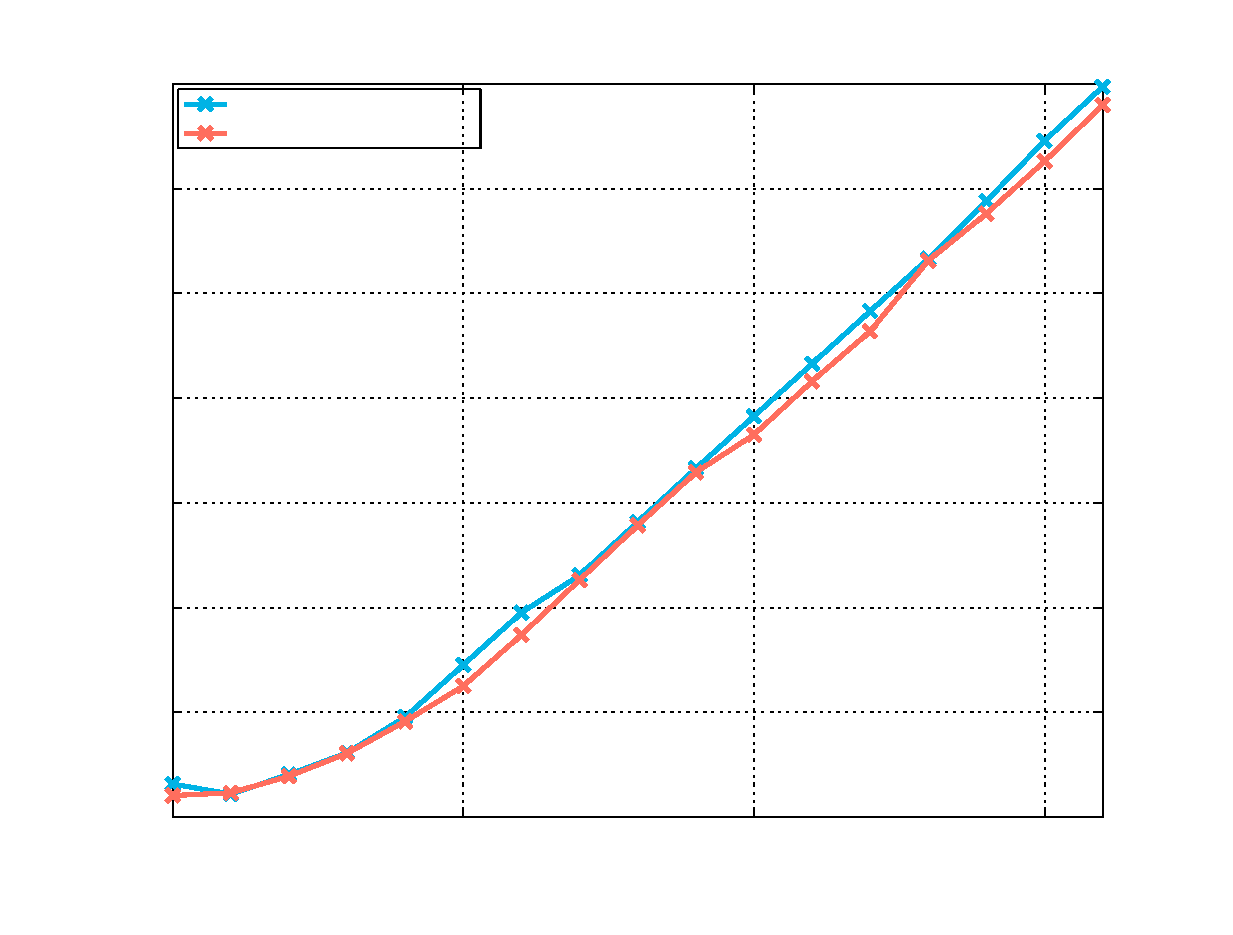
\includegraphics{consexp-inc}
\end{picture}%
\begin{picture}(576,433)(0,0)
\fontsize{10}{0}
\selectfont\put(74.88,43.5189){\makebox(0,0)[t]{\textcolor[rgb]{0,0,0}{{10}}}}
\fontsize{10}{0}
\selectfont\put(214.38,43.5189){\makebox(0,0)[t]{\textcolor[rgb]{0,0,0}{{15}}}}
\fontsize{10}{0}
\selectfont\put(353.88,43.5189){\makebox(0,0)[t]{\textcolor[rgb]{0,0,0}{{20}}}}
\fontsize{10}{0}
\selectfont\put(493.38,43.5189){\makebox(0,0)[t]{\textcolor[rgb]{0,0,0}{{25}}}}
\fontsize{10}{0}
\selectfont\put(69.8755,48.52){\makebox(0,0)[r]{\textcolor[rgb]{0,0,0}{{-10}}}}
\fontsize{10}{0}
\selectfont\put(69.8755,98.8172){\makebox(0,0)[r]{\textcolor[rgb]{0,0,0}{{-8}}}}
\fontsize{10}{0}
\selectfont\put(69.8755,149.114){\makebox(0,0)[r]{\textcolor[rgb]{0,0,0}{{-6}}}}
\fontsize{10}{0}
\selectfont\put(69.8755,199.411){\makebox(0,0)[r]{\textcolor[rgb]{0,0,0}{{-4}}}}
\fontsize{10}{0}
\selectfont\put(69.8755,249.709){\makebox(0,0)[r]{\textcolor[rgb]{0,0,0}{{-2}}}}
\fontsize{10}{0}
\selectfont\put(69.8755,300.006){\makebox(0,0)[r]{\textcolor[rgb]{0,0,0}{{0}}}}
\fontsize{10}{0}
\selectfont\put(69.8755,350.303){\makebox(0,0)[r]{\textcolor[rgb]{0,0,0}{{2}}}}
\fontsize{10}{0}
\selectfont\put(69.8755,400.6){\makebox(0,0)[r]{\textcolor[rgb]{0,0,0}{{4}}}}
\fontsize{10}{0}
\selectfont\put(298.08,32.5189){\makebox(0,0)[t]{\textcolor[rgb]{0,0,0}{{n}}}}
\fontsize{10}{0}
\selectfont\put(49.8755,224.56){\rotatebox{90}{\makebox(0,0)[b]{\textcolor[rgb]{0,0,0}{{logarithm of minimum runtime}}}}}
\fontsize{10}{0}
\selectfont\put(103.667,390.83){\makebox(0,0)[l]{\textcolor[rgb]{0,0,0}{{Dependently typed Version}}}}
\fontsize{10}{0}
\selectfont\put(103.667,376.775){\makebox(0,0)[l]{\textcolor[rgb]{0,0,0}{{Non-Dependently typed Version}}}}
\fontsize{10}{0}
\selectfont\put(298.08,410.6){\makebox(0,0)[b]{\textcolor[rgb]{0,0,0}{{Comparison of runtime for the cons experiment}}}}
\end{picture}
}
\end{figure}

\subsection{split}

This experiment is an extension of the previous one. In addition to constructing a \AgdaFunction{big-sequence}, we also invoke the \AgdaFunction{split} function in the form of \textit{get}(\AgdaFunction{\_!\_}). In order to obtain a non-trivial result, I am computing the time required to extract the middle element.

Since performing the \textit{get} operation requires creating a \AgdaFunction{big-sequence} in the same way as above, I have subtracted the results from the previous experiment, so that values reflect only the minimum time taken for the extraction of the middle element from increasingly long sequences.

\begin{figure}[H]
\caption{Splitting Experiment}
\scalebox{0.8} {
\begin{picture}(0,0)
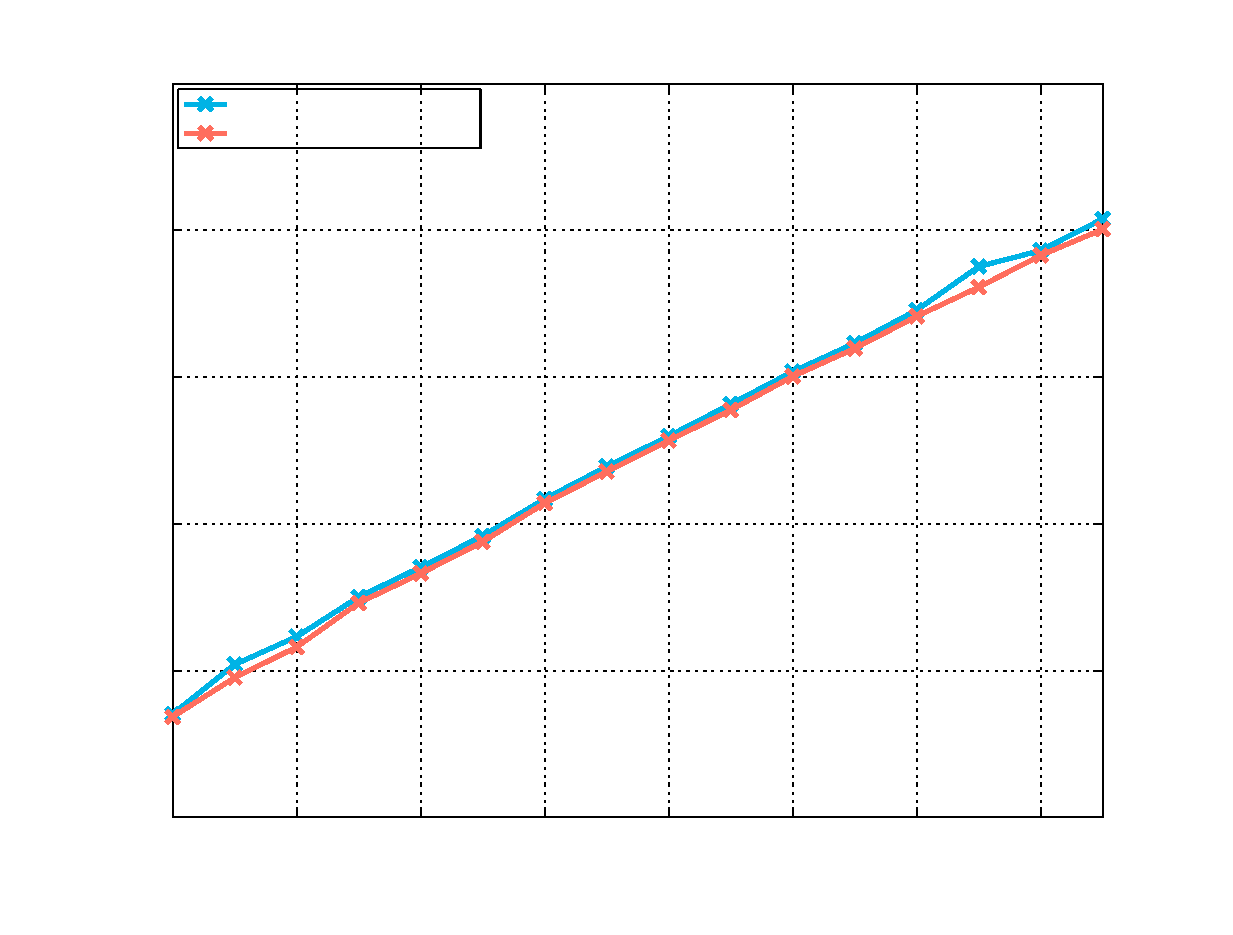
\includegraphics{splitexp-inc}
\end{picture}%
\begin{picture}(576,433)(0,0)
\fontsize{10}{0}
\selectfont\put(72.8,53.3083){\makebox(0,0)[t]{\textcolor[rgb]{0,0,0}{{10}}}}
\fontsize{10}{0}
\selectfont\put(130.667,53.3083){\makebox(0,0)[t]{\textcolor[rgb]{0,0,0}{{12}}}}
\fontsize{10}{0}
\selectfont\put(188.533,53.3083){\makebox(0,0)[t]{\textcolor[rgb]{0,0,0}{{14}}}}
\fontsize{10}{0}
\selectfont\put(246.4,53.3083){\makebox(0,0)[t]{\textcolor[rgb]{0,0,0}{{16}}}}
\fontsize{10}{0}
\selectfont\put(304.267,53.3083){\makebox(0,0)[t]{\textcolor[rgb]{0,0,0}{{18}}}}
\fontsize{10}{0}
\selectfont\put(362.133,53.3083){\makebox(0,0)[t]{\textcolor[rgb]{0,0,0}{{20}}}}
\fontsize{10}{0}
\selectfont\put(420,53.3083){\makebox(0,0)[t]{\textcolor[rgb]{0,0,0}{{22}}}}
\fontsize{10}{0}
\selectfont\put(477.867,53.3083){\makebox(0,0)[t]{\textcolor[rgb]{0,0,0}{{24}}}}
\fontsize{10}{0}
\selectfont\put(67.8,58.31){\makebox(0,0)[r]{\textcolor[rgb]{0,0,0}{{-15}}}}
\fontsize{10}{0}
\selectfont\put(67.8,126.933){\makebox(0,0)[r]{\textcolor[rgb]{0,0,0}{{-10}}}}
\fontsize{10}{0}
\selectfont\put(67.8,195.556){\makebox(0,0)[r]{\textcolor[rgb]{0,0,0}{{-5}}}}
\fontsize{10}{0}
\selectfont\put(67.8,264.179){\makebox(0,0)[r]{\textcolor[rgb]{0,0,0}{{0}}}}
\fontsize{10}{0}
\selectfont\put(67.8,332.802){\makebox(0,0)[r]{\textcolor[rgb]{0,0,0}{{5}}}}
\fontsize{10}{0}
\selectfont\put(67.8,401.425){\makebox(0,0)[r]{\textcolor[rgb]{0,0,0}{{10}}}}
\fontsize{10}{0}
\selectfont\put(289.8,42.3083){\makebox(0,0)[t]{\textcolor[rgb]{0,0,0}{{n}}}}
\fontsize{10}{0}
\selectfont\put(47.8,229.867){\rotatebox{90}{\makebox(0,0)[b]{\textcolor[rgb]{0,0,0}{{logarithm of minimum runtime}}}}}
\fontsize{10}{0}
\selectfont\put(100.787,391.904){\makebox(0,0)[l]{\textcolor[rgb]{0,0,0}{{Dependently Typed Version}}}}
\fontsize{10}{0}
\selectfont\put(100.787,378.206){\makebox(0,0)[l]{\textcolor[rgb]{0,0,0}{{Non-Dependently Typed Version}}}}
\fontsize{10}{0}
\selectfont\put(289.8,411.425){\makebox(0,0)[b]{\textcolor[rgb]{0,0,0}{{Comparison of runtime for the split experiment}}}}
\end{picture}
}
\end{figure}

It is clear from both these experiments that the dependently typed versions incur a higher computational cost. Moreover, the ends show that the divergence between the two depends on the input size.  However, this is not a limitation of dependent types, but of the compiler and extracting tools. All the type annotations could be removed without damaging correctness.

\subsection{reversing and problems with the compiler}

I have tried to repeat the same type of experiment, comparing the run-time of the \textbf{reverse-ft} method, implemented using \textbf{foldl}, and the \textit{rev} method, which uses the \textbf{ViewL}.

Unfortunately, the compilation of the latter method was not successful. Whereas the \textit{normalization} tool always returns the correct result, running a compiled version has caused a \textit{Segmentation Fault} error. This is quite damaging to the application, since a compiler that doesn't preserve the semantics of the code doesn't necessarily preserve correctness. 

\section{Heuristics for Effort}

There is no doubt that creating a dependently typed and verified version of a particular algorithm or data structure incurs an additional cost. In this section, I will try to explore the effort ratio between the implementing a simplistic solution versus a formally verified one. 

It is worth emphasising that, although computing or estimating efforts is in general an ill-defined task, some heuristics could help compare the different versions of the same data structure and see if the figures carry on across data structures.

I have suggested using two heuristics, one computing the explosion in SLOC\footnote{Source Lines of Code}, and the other one quantifying the axiom and lemma content in the definitions.

\subsection{Lines of code}

I will present the ratio between the lengths of different versions, commenting on what they achieve. Although arguably, counting lines of code is not always representative, in this case it seems suitable since: 
\begin{itemize}
\item All the presented code has been written by a single programmer\footnote{It is debatable whether the metrics will show something about using dependent types or just about myself as a programmer.}.
\item I have been consistent with jumping to new lines.
\end{itemize}
	
I will make a clear distinction between \textit{internal} verification and \textit{external} verification \cite{verifagda}. By the former I mean properties that are made clear through the type of the definitions themselves (e.g. the use of measure as an index), while the latter refers to proofs which are carried outside of the definition (e.g. foldl-correct).

For this metric, I have decided to discard all the \textit{external}ly verified properties, since there is no bound on their number. On the other hand, \textit{internal} verification directly affects the implementation's difficulty.

Furthermore, I will categorise the lines in four categories. \textbf{Type annotations} (declaring the function about to be defined as well as data declarations), \textbf{Implementation} (definitions of functions that are relevant to the implementation), \textbf{Proofs} (lines related to proofs and the calls to them), \textbf{Other} (importing modules, \textit{where} clauses etc.).
  
\paragraph{Selection Sort.}

The selection sort procedure, presented in section \ref{par:sort}, is an example of a fully formally verified procedure, as all that can be expected of a sorting function is encoded in the type system. This differs from the FingerTree implementation, which only enforces correctness of the measurement.

\begin{table}[H]
\caption{SLOC for Sorting}
\center
\begin{tabular}{c r r}
\hline
Content & Verified & Not Verified\\
\hline
Implementation & 18 & 14 \\
Type annotations & 24 & 3 \\
Proofs & 124 & 0 \\
Other & 53 & 50 \\
Total & 219 & 67 \\
\hline
\end{tabular} 
\end{table}

The non-verified example in this case does not run in Agda. It would require proofs of termination. I have only presented this as a reference point for the FingerTree example.

\paragraph{FingerTree.}

\begin{table}[H]
\caption{SLOC for FingerTree}
\center
\begin{tabular}{c r r}
\hline 
Content & Measured Version & Size Version \\
\hline
Implementation & 185 & 162 \\ 
Type annotations & 195 & 100 \\
%Type annotations & 144 & 68 \\ 
%Data declarations & 51 & 32 \\
Proofs & 350 & 30 \\
Other & 30 & 22 \\ 
Total & 760 & 314 \\
\hline
\end{tabular}
\end{table} 

It is interesting to see the same ratios remaining consistent. As a sanity check, the code related to implementation has stayed constant. The proofs carry around half of the code for a verified version. This depends of course on the number of invariants we are trying to maintain. A further increase in the lines that express type signature lead to an overall 2.5 factor of explosion in the code. 

In the dependently typed setting, the Implementation and Type annotation carry almost equal weight, in contrast to a 3:1 ratio in the non-dependently typed one.

However, the effort, as illustrated here, is not directly related to difficulty, since the more expressive types in verified versions make the goals of implementation clearer. 

At the beginning of the project, I was expecting that the automatic proof search tool would make a great difference \cite{auto}. Unfortunately, the cases in which it returned results were very few in most of the files, and nonexistent in the implementation of the dependent FingerTree. 

Some proofs were not included here, due to the fact that to derive them I used a reimplementation of the MonoidSolver (required because of incompatibilities with the standard library). This automates the proof through the use of reflection \cite{reflection}. Such proofs are constructed at compile time and I could observe them using normalization. Unfortunately, they are considerably longer than the other proofs I have written, so including them would have made this analysis inconsistent.

\subsection{Lemma Usage}
\label{eval:lemma}
The previous examples did not include any metric about the externally verified properties. 
Performing this evaluation experiment showed that all the lemmas are constructed from calls to our assumptions (base lemmas).

\begin{itemize}
\item about the equivalence relation: \textit{refl}, \textit{sym}, \textit{cong} and \textit{trans}
\item about the monoid relation: \textit{associativity}, $\epsilon$ is \textit{neutral element}
\item about List: \textit{associativity} of \textit{++} and \textit{[]} is \textit{neutral element}
\end{itemize} 

I have performed an analysis of which lemmas are being used by each declaration, followed by a flattening of the result to the base lemmas. The final numbers can be seen as a metric of effort, but also a potential starting point for refactoring. A summary of results is given below:

\begin{table}[H]
\caption{Lemma Usage for Internal Verification}
\center
\begin{tabular}{c r r r r r}
\hline 
Lemma & cons & snoc & viewL & viewR & split \\
\hline
refl  	&	1	&	0	&	3&	3&  48\\
sym     &	2	&	16	&	5&	8&	23\\
cong   	&	3	&	11	&	1&	5&	15\\
trans  	&	3	&	23	&	6&	10& 46\\
ε-left  &	1	&	2	&	4&	2& 22\\  
ε-right &	1	&	0	&	2&	4& 13\\
$∙$-assoc &	6	&	18	&	3&	8& 21\\
\hline
\end{tabular}
\end{table} 

This graph suggests two things. First of all, due to the declaration of the monoid operator as \textbf{infixl}, the operations that have a right-associative structure tend to be easier to prove. This creates a contrast between cons and viewL on one side and snoc and viewR on the other. 

I believe that the split operation is even more difficult because apart from taking over the difficulties of both viewL and viewR, it also combines two different types of logical statement. 

Although we only rely on the Curry Howard Isomorphism, the alternative reasoning also incorporates the Boolean data type and its associated operations (and, or, negation). Instead of proceeding as before, using: 
 
\begin{code}
\\
\>[0]\AgdaIndent{2}{}\<[2]%
\>[2]\AgdaFunction{proof-istrue} \AgdaSymbol{:} \AgdaSymbol{∀} \AgdaBound{a} \AgdaSymbol{→} \AgdaPostulate{property} \AgdaBound{a}\<%
\\
\>[0]\AgdaIndent{2}{}\<[2]%
\>[2]\AgdaFunction{proof-isfalse} \AgdaSymbol{:} \AgdaSymbol{∀} \AgdaBound{a} \AgdaSymbol{→} \AgdaSymbol{(}\AgdaPostulate{property} \AgdaBound{a} \AgdaSymbol{→} \AgdaPostulate{⊥}\AgdaSymbol{)}\<%
\\
\end{code} 

We now also make use of: 

\begin{code}
\\
\>[0]\AgdaIndent{2}{}\<[2]%
\>[2]\AgdaFunction{pred-istrue} \AgdaSymbol{:} \AgdaSymbol{∀} \AgdaBound{a} \AgdaSymbol{→} \AgdaSymbol{(}\AgdaPostulate{predicate} \AgdaBound{a} \AgdaDatatype{≡} \AgdaInductiveConstructor{true}\AgdaSymbol{)}\<%
\\
\>[0]\AgdaIndent{2}{}\<[2]%
\>[2]\AgdaFunction{pred-isfalse} \AgdaSymbol{:} \AgdaSymbol{∀} \AgdaBound{a} \AgdaSymbol{→} \AgdaSymbol{(}\AgdaPostulate{predicate} \AgdaBound{a} \AgdaDatatype{≡} \AgdaInductiveConstructor{false}\AgdaSymbol{)}\<%
\\
\end{code}

This inconvenience became more noticeable when I tried to port the Isabelle implementation \cite{isabelle}, which is not based on dependent types. Although they can be fully encoded, the proofs become long due to the lack of type checking support. Some examples of this are in the Appendix \ref{app:sort}. This would perhaps be a starting point for some future work.

\section{Discussion}

As part of the introduction, I posed a question related to how far Agda's expressivity can take us in the implementation of a functional data structure.

In relation to Matthieu Souzeau's paper \cite{coq}, I have completed the implementations of all the operations he suggested. Furthermore, I have presented an Agda way to deal with the termination checking problem, discussed in his section 4.4.1 Dependence Hell. 
It is interesting to notice that this problem is not strictly related to Agda, but to a wider family of dependently typed languages.  

In addition, I have also explicitly proven axioms that relate FingerTrees to their list representation.


\chapter{Conclusion}

\section{Accomplishments}

In this dissertation, I have successfully implemented the FingerTree data structure \cite{fingertrees} in Agda \cite{agdatutorial} and provided verified definitions for the data structure described in Table \ref{tab:operations}. The results were similar to those obtained by Mattheiu Souzeau \cite{coq}, as both implementations suffered from the same limitations. From this, I draw the conclusion that even though Coq is a richer platform, it does not necessarily achieve more, especially in cases when simplicity is important. The inferiority of proof automation could become a blessing in disguise in Agda, since the development of the FingerTree almost lead me to rediscover the proof by reflection employed in the MonoidSolver. \\
I managed to outline and give extensive examples to the problem \textit{Sized Types} can cause when combined with functions on nested types. The source of the difficulty has been pointed out as being firstly because of the lack of pattern matching support and secondly due to the creation of negative cycles in the sizing graph. 
I have discussed the termination-checking limitation of dependently-typed theorem provers, and also presented an Agda implementation of the solution suggested in \cite{coq} in Section \ref{sec:wfrec}. \\
In order to achieve these results, I have provided a concise introduction to Agda and programming with dependent types, as well as examples of proofs and other similar data structures where the same issues occur (included in the Appendix due to size constraints).
I have evaluated the implementations, as well as provided some insight into the difficulty of developing proofs in Agda. Furthermore, I have managed to compile a substantial fragment of the relevant literature and provide satisfying examples that connect the essential concepts. 

\section{Further work}

In the course of developing this dissertation, I have noticed some Agda limitations. I have illustrated them throughout the previous sections. They are all potential starting points for future work:

\begin{itemize}
\item Type-checking within \AgdaKeyword{with} abstracted statements.
\item Use of \textit{Sized Types} for nested types.
\item Compilation limitations.
\end{itemize} \hfill

\noindent Considering the implementation itself, I can make the following suggestions:

\begin{itemize}

\item With regard to my original proposition of packaging the implementation in a library -- the outcome of this project could have easily been included in the standard library, had I used the already implemented Monoid record and universe level conventions. This is a straightforward extension that could be carried out and would benefit the community.

\item Auxiliary constraints of the measuring function would allow writing recursive definitions using the approach presented in Section \ref{sec:wfrec}. One could enforce that:

\begin{code}
\>[4]\AgdaIndent{6}{}\<[6]%
\>[6]\AgdaField{mpos} \AgdaSymbol{:} \AgdaSymbol{∀} \AgdaBound{x} \AgdaSymbol{→} \AgdaFunction{ε} \AgdaBound{>} \AgdaField{∥} \AgdaBound{x} \AgdaField{∥}\<%
\end{code} 
This would ensure that adding a new element to the FingerTree yields one with a bigger size (where bigger is given by the \_>\_ relation), formally by ensuring that: $\forall$ s : V, x : A. s $∙ \Vert x \Vert$ > s. This allows writing arbitrary recursive definitions using the paradigm from Section \ref{sec:wfrec}.
 
\item Related to the discussion about the Isabelle implementation \cite{isabelle} and porting it fully to Agda, I believe that a module similar to the Propositional Equality can be implemented to facilitate doing proofs of the type:
 
\indent \AgdaPostulate{predicate} \AgdaBound{a} \AgdaDatatype{≡} \AgdaInductiveConstructor{false}
\end{itemize}

\section{Lessons learned}

During this project, I have familiarised myself with Agda, and gained sufficient insight into type theory to be able to read and understand cutting edge research. I have acquired invaluable experience in formal verification and its application to testing or prototyping data structures. 
Successful verification requires some practice in order to get used to the environment's quirks, as in many cases a well chosen definitions for theorems is key to the process. 

The field of formal verification using dependent types is slowly entering the industry, through the advent of more accessible programming languages like Agda, Idris or Dependent Haskell. Although still young, such tools show potential and are surrounded by active communities. I have shown, through implementing a non trivial data structure, the trade-off between expressivity and limitations in Agda, and I hope that I have inspired further work and study in this area.

\chapter{Appendix}

%TC:ignore
\section{Helper Functions}
\label{app:helper}
\begin{itemize}

\item Flattening a list of Node A V to a list of A, by repeatedly transforming nodes to lists and aggregating the result.\\
\begin{code}
\\
\>\AgdaFunction{flatten-list} \AgdaSymbol{:} \AgdaSymbol{∀} \AgdaSymbol{\{}\AgdaBound{a}\AgdaSymbol{\}\{}\AgdaBound{A} \AgdaSymbol{:} \AgdaPrimitiveType{Set} \AgdaBound{a}\AgdaSymbol{\}\{}\AgdaBound{V} \AgdaSymbol{:} \AgdaPrimitiveType{Set} \AgdaBound{a} \AgdaSymbol{\}}\<%
\\
\>[6]\AgdaIndent{14}{}\<[14]%
\>[14]\AgdaSymbol{⦃} \AgdaBound{mo} \AgdaSymbol{:} \AgdaRecord{Monoid} \AgdaBound{V} \AgdaSymbol{⦄}\<%
\\
\>[6]\AgdaIndent{14}{}\<[14]%
\>[14]\AgdaSymbol{⦃} \AgdaBound{m} \AgdaSymbol{:} \AgdaRecord{Measured} \AgdaBound{A} \AgdaBound{V} \AgdaSymbol{⦄}\<%
\\
\>[6]\AgdaIndent{14}{}\<[14]%
\>[14]\AgdaSymbol{→} \AgdaDatatype{List} \AgdaSymbol{(}\AgdaDatatype{Node} \AgdaBound{A} \AgdaBound{V}\AgdaSymbol{)}\<%
\\
\>[6]\AgdaIndent{14}{}\<[14]%
\>[14]\AgdaSymbol{→} \AgdaDatatype{List} \AgdaBound{A}\<%
\\
\>\AgdaFunction{flatten-list} \AgdaInductiveConstructor{[]} \AgdaSymbol{=} \AgdaInductiveConstructor{[]}\<%
\\
\>\AgdaFunction{flatten-list} \AgdaSymbol{(}\AgdaBound{x} \AgdaInductiveConstructor{∷} \AgdaBound{xs}\AgdaSymbol{)} \AgdaSymbol{=} \AgdaSymbol{(}\AgdaFunction{toList-node} \AgdaBound{x}\AgdaSymbol{)} \AgdaFunction{++} \AgdaSymbol{(}\AgdaFunction{flatten-list} \AgdaBound{xs}\AgdaSymbol{)}\<%
\\
\end{code}


\end{itemize}
\section{Numerical Representations}
\label{app:numrep}
The treatment of containers as natural numbers has been studied in depth\cite{okasaki}. The basic idea is that simple numerical operations correspond naturally to operations on containers. For example:

\vspace{5mm} %5mm vertical space 
\begin{tabular}{lcl}
increasing a number & corresponds to & adding an element\\
decreasing a number & corresponds to & removing an element \\
adding two numbers & corresponds to & merging to containers \\
\end{tabular} 
\vspace{5mm}

This treatment of numbers, represented in various numerical basis, allows the constructions the obey the implicit recursive slowdown, presented by okasaki. This allows in lazy languages like Haskell, implementation of operations such as insertion and deletion in ammortised O(1) cost -- which represented a breakthrough in functional programming languages.

\section{Further example of the termination checking limitation}
\label{app:termcheck}
In this section, I will present a data structure as implemented by Ralf Hinze\cite{nestedhinze} and show the issues that could arise because of the termination checker in more detail. 

Consider the trivial implementation of a binary tree in a functional programming language:

\begin{code}
\\
\>[2]\AgdaIndent{4}{}\<[4]%
\>[4]\AgdaKeyword{data} \AgdaDatatype{Bush} \AgdaSymbol{(}\AgdaBound{A} \AgdaSymbol{:} \AgdaPrimitiveType{Set}\AgdaSymbol{)} \AgdaSymbol{:} \AgdaPrimitiveType{Set} \AgdaKeyword{where}\<%
\\
\>[4]\AgdaIndent{6}{}\<[6]%
\>[6]\AgdaInductiveConstructor{Leaf} \AgdaSymbol{:} \AgdaBound{A} \AgdaSymbol{→} \AgdaDatatype{Bush} \AgdaBound{A}\<%
\\
\>[4]\AgdaIndent{6}{}\<[6]%
\>[6]\AgdaInductiveConstructor{Fork} \AgdaSymbol{:} \AgdaDatatype{Bush} \AgdaBound{A} \AgdaSymbol{→} \AgdaDatatype{Bush} \AgdaBound{A} \AgdaSymbol{→} \AgdaDatatype{Bush} \AgdaBound{A}\<%
\\
\end{code}

In order to stay consistent with the original implementation, the data structure above will be split in two different types that represent the constructors \cite{numerical}.

%-- constructors.
\begin{code}
\\
\>[2]\AgdaIndent{4}{}\<[4]%
\>[4]\AgdaKeyword{data} \AgdaDatatype{Leaf} \AgdaSymbol{(}\AgdaBound{A} \AgdaSymbol{:} \AgdaPrimitiveType{Set}\AgdaSymbol{)} \AgdaSymbol{:} \AgdaPrimitiveType{Set} \AgdaKeyword{where}\<%
\\
\>[4]\AgdaIndent{6}{}\<[6]%
\>[6]\AgdaInductiveConstructor{LEAF} \AgdaSymbol{:} \AgdaBound{A} \AgdaSymbol{→} \AgdaDatatype{Leaf} \AgdaBound{A}\<%
\\
%
\\
\>[0]\AgdaIndent{4}{}\<[4]%
\>[4]\AgdaKeyword{data} \AgdaDatatype{Fork} \AgdaSymbol{(}\AgdaBound{B} \AgdaSymbol{:} \AgdaPrimitiveType{Set} \AgdaSymbol{→} \AgdaPrimitiveType{Set}\AgdaSymbol{)(}\AgdaBound{A} \AgdaSymbol{:} \AgdaPrimitiveType{Set}\AgdaSymbol{)} \AgdaSymbol{:} \AgdaPrimitiveType{Set} \AgdaKeyword{where}\<%
\\
\>[4]\AgdaIndent{6}{}\<[6]%
\>[6]\AgdaInductiveConstructor{FORK} \AgdaSymbol{:} \AgdaSymbol{(}\AgdaBound{B} \AgdaBound{A}\AgdaSymbol{)} \AgdaSymbol{→} \AgdaSymbol{(}\AgdaBound{B} \AgdaBound{A}\AgdaSymbol{)} \AgdaSymbol{→} \AgdaDatatype{Fork} \AgdaBound{B} \AgdaBound{A}\<%
\\
\end{code}


We can now refer to the Random Access Sequence implementation.
They are a numerical representation based on base two of natural numbers, however, rather than the 0-1 system, the author prefers to use the 1-2 system for a number of effiency reasons.

\begin{center}
	\begin{tabular}{lcl}
	$inc(\epsilon$) & = & $1$ \\
	$inc(1a)$ & = & $2a$ \\ 
	$inc(2a)$ & = & $1inc(a)$ \\
	\end{tabular} 
\end{center}

This $inc$ operator should correspond analogously to the 'Cons' operators in the data structure:

%--RAL
\begin{code}
\\
\>[0]\AgdaIndent{4}{}\<[4]%
\>[4]\AgdaKeyword{data} \AgdaDatatype{RandomAccessList} \AgdaSymbol{(}\AgdaBound{B} \AgdaSymbol{:} \AgdaPrimitiveType{Set} \AgdaSymbol{→} \AgdaPrimitiveType{Set}\AgdaSymbol{)} \AgdaSymbol{(}\AgdaBound{A} \AgdaSymbol{:} \AgdaPrimitiveType{Set}\AgdaSymbol{)} \AgdaSymbol{:} \AgdaPrimitiveType{Set} \AgdaKeyword{where}\<%
\\
\>[4]\AgdaIndent{6}{}\<[6]%
\>[6]\AgdaInductiveConstructor{Nil} \AgdaSymbol{:} \AgdaDatatype{RandomAccessList} \AgdaBound{B} \AgdaBound{A}\<%
\\
\>[4]\AgdaIndent{6}{}\<[6]%
\>[6]\AgdaInductiveConstructor{One} \AgdaSymbol{:} \AgdaSymbol{(}\AgdaBound{B} \AgdaBound{A}\AgdaSymbol{)} \AgdaSymbol{→} \AgdaSymbol{(}\AgdaDatatype{RandomAccessList} \AgdaSymbol{(}\AgdaDatatype{Fork} \AgdaBound{B}\AgdaSymbol{)} \AgdaBound{A}\AgdaSymbol{)} \AgdaSymbol{→} \AgdaDatatype{RandomAccessList} \AgdaBound{B} \AgdaBound{A}\<%
\\
\>[4]\AgdaIndent{6}{}\<[6]%
\>[6]\AgdaInductiveConstructor{Two} \AgdaSymbol{:} \AgdaSymbol{(}\AgdaDatatype{Fork} \AgdaBound{B} \AgdaBound{A}\AgdaSymbol{)} \AgdaSymbol{→} \AgdaSymbol{(}\AgdaDatatype{RandomAccessList} \AgdaSymbol{(}\AgdaDatatype{Fork} \AgdaBound{B}\AgdaSymbol{)} \AgdaBound{A}\AgdaSymbol{)} \AgdaSymbol{→} \AgdaDatatype{RandomAccessList} \AgdaBound{B} \AgdaBound{A}\<%
\\
\end{code}

Now, by implementing the function $incr$, we can see the similarity between the adding an element to the left and the number representation 

\begin{code}
\\
\>[0]\AgdaIndent{4}{}\<[4]%
\>[4]\AgdaFunction{incr} \AgdaSymbol{:} \AgdaSymbol{\{}\AgdaBound{B} \AgdaSymbol{:} \AgdaPrimitiveType{Set} \AgdaSymbol{→} \AgdaPrimitiveType{Set}\AgdaSymbol{\}} \AgdaSymbol{\{}\AgdaBound{A} \AgdaSymbol{:} \AgdaPrimitiveType{Set}\AgdaSymbol{\}} \AgdaSymbol{→} \AgdaSymbol{(}\AgdaBound{B} \AgdaBound{A}\AgdaSymbol{)}\<%
\\
\>[4]\AgdaIndent{10}{}\<[10]%
\>[10]\AgdaSymbol{→} \AgdaDatatype{RandomAccessList} \AgdaBound{B} \AgdaBound{A}\<%
\\
\>[4]\AgdaIndent{10}{}\<[10]%
\>[10]\AgdaSymbol{→} \AgdaDatatype{RandomAccessList} \AgdaBound{B} \AgdaBound{A}\<%
\\
\>[0]\AgdaIndent{4}{}\<[4]%
\>[4]\AgdaFunction{incr} \AgdaBound{b} \AgdaInductiveConstructor{Nil} \AgdaSymbol{=} \AgdaInductiveConstructor{One} \AgdaBound{b} \AgdaInductiveConstructor{Nil}\<%
\\
\>[0]\AgdaIndent{4}{}\<[4]%
\>[4]\AgdaFunction{incr} \AgdaBound{b} \AgdaSymbol{(}\AgdaInductiveConstructor{One} \AgdaBound{b₂} \AgdaBound{ds}\AgdaSymbol{)} \AgdaSymbol{=} \AgdaInductiveConstructor{Two} \AgdaSymbol{(}\AgdaInductiveConstructor{FORK} \AgdaBound{b} \AgdaBound{b₂}\AgdaSymbol{)} \AgdaBound{ds}\<%
\\
\>[0]\AgdaIndent{4}{}\<[4]%
\>[4]\AgdaFunction{incr} \AgdaBound{b} \AgdaSymbol{(}\AgdaInductiveConstructor{Two} \AgdaBound{b₂} \AgdaBound{ds}\AgdaSymbol{)} \AgdaSymbol{=} \AgdaInductiveConstructor{One} \AgdaBound{b} \AgdaSymbol{(}\AgdaFunction{incr} \AgdaBound{b₂} \AgdaBound{ds}\AgdaSymbol{)}\<%
\\
\end{code}
Following, I declare the sequence by using the definition of Leaf as a layer of abstraction.

\begin{code}
\\
\>[0]\AgdaIndent{4}{}\<[4]%
\>[4]\AgdaFunction{IxSequence} \AgdaSymbol{:} \AgdaPrimitiveType{Set} \AgdaSymbol{→} \AgdaPrimitiveType{Set}\<%
\\
\>[0]\AgdaIndent{4}{}\<[4]%
\>[4]\AgdaFunction{IxSequence} \AgdaSymbol{=} \AgdaDatatype{RandomAccessList} \AgdaDatatype{Leaf}\<%
\\
\\
\>[0]\AgdaIndent{4}{}\<[4]%
\>[4]\AgdaFunction{cons} \AgdaSymbol{:} \AgdaSymbol{\{}\AgdaBound{A} \AgdaSymbol{:} \AgdaPrimitiveType{Set}\AgdaSymbol{\}} \AgdaSymbol{→} \AgdaBound{A} \AgdaSymbol{→} \AgdaFunction{IxSequence} \AgdaBound{A} \AgdaSymbol{→} \AgdaFunction{IxSequence} \AgdaBound{A}\<%
\\
\>[0]\AgdaIndent{4}{}\<[4]%
\>[4]\AgdaFunction{cons} \AgdaBound{a} \AgdaBound{s} \AgdaSymbol{=} \AgdaFunction{incr} \AgdaSymbol{(}\AgdaInductiveConstructor{LEAF} \AgdaBound{a}\AgdaSymbol{)} \AgdaBound{s}\<%
\\
\end{code}

\subsection{Defining a view} 

We can then implement the $front$ method, which returns a view of the list in terms of the first element and a continutation. Our goal is to abstract away the intricacy of the type declaration, so we can implement methods  easily. First, we need to declare the return type, wrapped in a view data structure.

%--View %--front

\begin{code}
\\
\>[0]\AgdaIndent{4}{}\<[4]%
\>[4]\AgdaKeyword{data} \AgdaDatatype{View} \AgdaSymbol{(}\AgdaBound{A} \AgdaSymbol{:} \AgdaPrimitiveType{Set}\AgdaSymbol{)} \AgdaSymbol{:} \AgdaPrimitiveType{Set} \AgdaKeyword{where}\<%
\\
\>[4]\AgdaIndent{6}{}\<[6]%
\>[6]\AgdaInductiveConstructor{Vnil} \AgdaSymbol{:} \AgdaDatatype{View} \AgdaBound{A}\<%
\\
\>[4]\AgdaIndent{6}{}\<[6]%
\>[6]\AgdaInductiveConstructor{VCns} \AgdaSymbol{:} \AgdaBound{A} \AgdaFunction{×} \AgdaFunction{IxSequence} \AgdaBound{A} \AgdaSymbol{→} \AgdaDatatype{View} \AgdaBound{A}\<%
\\
%
\\
\>[0]\AgdaIndent{4}{}\<[4]%
\>[4]\AgdaFunction{front} \AgdaSymbol{:} \AgdaSymbol{\{}\AgdaBound{A} \AgdaSymbol{:} \AgdaPrimitiveType{Set}\AgdaSymbol{\}} \AgdaSymbol{→} \AgdaFunction{IxSequence} \AgdaBound{A} \AgdaSymbol{→} \AgdaDatatype{View} \AgdaBound{A}\<%
\\
\>[0]\AgdaIndent{4}{}\<[4]%
\>[4]\AgdaFunction{front} \AgdaInductiveConstructor{Nil} \AgdaSymbol{=} \AgdaInductiveConstructor{Vnil}\<%
\\
\>[0]\AgdaIndent{4}{}\<[4]%
\>[4]\AgdaFunction{front} \AgdaSymbol{(}\AgdaInductiveConstructor{One} \AgdaSymbol{(}\AgdaInductiveConstructor{LEAF} \AgdaBound{x}\AgdaSymbol{)} \AgdaBound{ds}\AgdaSymbol{)} \AgdaSymbol{=} \AgdaInductiveConstructor{VCns} \AgdaSymbol{(}\AgdaBound{x} \AgdaInductiveConstructor{,} \AgdaFunction{zero} \AgdaBound{ds}\AgdaSymbol{)}\<%
\\
\>[0]\AgdaIndent{4}{}\<[4]%
\>[4]\AgdaFunction{front} \AgdaSymbol{(}\AgdaInductiveConstructor{Two} \AgdaSymbol{(}\AgdaInductiveConstructor{FORK} \AgdaSymbol{(}\AgdaInductiveConstructor{LEAF} \AgdaBound{a}\AgdaSymbol{)} \AgdaBound{b}\AgdaSymbol{)} \AgdaBound{ds}\AgdaSymbol{)} \AgdaSymbol{=} \AgdaInductiveConstructor{VCns} \AgdaSymbol{(}\AgdaBound{a} \AgdaInductiveConstructor{,} \AgdaInductiveConstructor{One} \AgdaBound{b} \AgdaBound{ds}\AgdaSymbol{)}\<%
\\
\end{code}

The zero method is a restructuring method, as we will find in the FingerTree implementation.

\begin{code}
\\
\>[0]\AgdaIndent{4}{}\<[4]%
\>[4]\AgdaFunction{zero} \AgdaSymbol{:} \AgdaSymbol{\{}\AgdaBound{B} \AgdaSymbol{:} \AgdaPrimitiveType{Set} \AgdaSymbol{→} \AgdaPrimitiveType{Set}\AgdaSymbol{\}} \AgdaSymbol{\{}\AgdaBound{A} \AgdaSymbol{:} \AgdaPrimitiveType{Set}\AgdaSymbol{\}} \AgdaSymbol{→}\<%
\\
\>[4]\AgdaIndent{6}{}\<[6]%
\>[6]\AgdaDatatype{RandomAccessList} \AgdaSymbol{(}\AgdaDatatype{Fork} \AgdaBound{B}\AgdaSymbol{)} \AgdaBound{A} \AgdaSymbol{→}\<%
\\
\>[4]\AgdaIndent{6}{}\<[6]%
\>[6]\AgdaDatatype{RandomAccessList} \AgdaBound{B} \AgdaBound{A}\<%
\\
\>[0]\AgdaIndent{4}{}\<[4]%
\>[4]\AgdaFunction{zero} \AgdaInductiveConstructor{Nil} \AgdaSymbol{=} \AgdaInductiveConstructor{Nil}\<%
\\
\>[0]\AgdaIndent{4}{}\<[4]%
\>[4]\AgdaFunction{zero} \AgdaSymbol{(}\AgdaInductiveConstructor{One} \AgdaBound{b} \AgdaBound{ds}\AgdaSymbol{)} \AgdaSymbol{=} \AgdaInductiveConstructor{Two} \AgdaBound{b} \AgdaSymbol{(}\AgdaFunction{zero} \AgdaBound{ds}\AgdaSymbol{)}\<%
\\
\>[0]\AgdaIndent{4}{}\<[4]%
\>[4]\AgdaFunction{zero} \AgdaSymbol{(}\AgdaInductiveConstructor{Two} \AgdaSymbol{(}\AgdaInductiveConstructor{FORK} \AgdaBound{b₁} \AgdaBound{b₂}\AgdaSymbol{)} \AgdaBound{ds}\AgdaSymbol{)} \AgdaSymbol{=} \AgdaInductiveConstructor{Two} \AgdaBound{b₁} \AgdaSymbol{(}\AgdaInductiveConstructor{One} \AgdaBound{b₂} \AgdaBound{ds}\AgdaSymbol{)}\<%
\\
\end{code} 

\subsection{Example termination failure}

Here, Agda termination checker will fail. We will try to implement an append function, which is a straightforward process given the methods previously declared:

\begin{code}
\\
\>[0]\AgdaIndent{4}{}\<[4]%
\>[4]\AgdaFunction{append} \AgdaSymbol{:} \AgdaSymbol{\{}\AgdaBound{A} \AgdaSymbol{:} \AgdaPrimitiveType{Set}\AgdaSymbol{\}} \AgdaSymbol{→} \AgdaBound{A} \AgdaSymbol{→} \AgdaFunction{IxSequence} \AgdaBound{A} \AgdaSymbol{→} \AgdaFunction{IxSequence} \AgdaBound{A}\<%
\\
\>[0]\AgdaIndent{4}{}\<[4]%
\>[4]\AgdaFunction{append} \AgdaBound{x} \AgdaBound{seq} \AgdaKeyword{with} \AgdaFunction{front} \AgdaBound{seq}\<%
\\
\>[0]\AgdaIndent{4}{}\<[4]%
\>[4]\AgdaFunction{append} \AgdaBound{x} \AgdaBound{seq} \AgdaSymbol{|} \AgdaInductiveConstructor{Vnil} \AgdaSymbol{=} \AgdaFunction{cons} \AgdaBound{x} \AgdaInductiveConstructor{Nil}\<%
\\
\>[0]\AgdaIndent{4}{}\<[4]%
\>[4]\AgdaFunction{append} \AgdaBound{x} \AgdaBound{seq} \AgdaSymbol{|} \AgdaInductiveConstructor{VCns} \AgdaSymbol{(}\AgdaBound{head} \AgdaInductiveConstructor{,} \AgdaBound{tail}\AgdaSymbol{)} \AgdaSymbol{=} \AgdaFunction{cons} \AgdaBound{head} \AgdaSymbol{(}\AgdaFunction{append} \AgdaBound{x} \AgdaBound{tail}\AgdaSymbol{)}\<%
\\
\end{code}

\subsection{Using sized types}

Sized types are agda's response to fixing such issues. However, trying to come up with an implementation that type checks, even in this relatively simple case seems to be very difficult. The intuition in this case is that we need to convince agda that FORK a b is bigger than any individual a b in the context of the RAL constructors. However, sized types are only relative, not on an absolute scale.

\begin{code}
\\
\>[0]\AgdaIndent{4}{}\<[4]%
\>[4]\AgdaKeyword{data} \AgdaDatatype{RandomAccessList} \AgdaSymbol{(}\AgdaBound{B} \AgdaSymbol{:} \AgdaPrimitiveType{Set} \AgdaSymbol{→} \AgdaPrimitiveType{Set}\AgdaSymbol{)(}\AgdaBound{A} \AgdaSymbol{:} \AgdaPrimitiveType{Set}\AgdaSymbol{)} \AgdaSymbol{:} \AgdaSymbol{\{}\AgdaBound{i} \AgdaSymbol{:} \AgdaPostulate{Size}\AgdaSymbol{\}} \AgdaSymbol{→} \AgdaPrimitiveType{Set} \AgdaKeyword{where}\<%
\\
\>[4]\AgdaIndent{6}{}\<[6]%
\>[6]\AgdaInductiveConstructor{Nil} \AgdaSymbol{:} \AgdaSymbol{∀} \AgdaSymbol{\{}\AgdaBound{i}\AgdaSymbol{\}} \AgdaSymbol{→} \AgdaDatatype{RandomAccessList} \AgdaBound{B} \AgdaBound{A} \AgdaSymbol{\{}\AgdaBound{i}\AgdaSymbol{\}}\<%
\\
\>[4]\AgdaIndent{6}{}\<[6]%
\>[6]\AgdaInductiveConstructor{One} \AgdaSymbol{:} \AgdaSymbol{∀} \AgdaSymbol{\{}\AgdaBound{i}\AgdaSymbol{\}} \AgdaSymbol{→} \AgdaSymbol{(}\AgdaBound{B} \AgdaBound{A}\AgdaSymbol{)} \AgdaSymbol{→} \AgdaSymbol{(}\AgdaDatatype{RandomAccessList} \AgdaSymbol{(}\AgdaDatatype{Fork} \AgdaBound{B}\AgdaSymbol{)} \AgdaBound{A} \AgdaSymbol{\{}\AgdaBound{i}\AgdaSymbol{\})}\<%
\\
\>[6]\AgdaIndent{26}{}\<[26]%
\>[26]\AgdaSymbol{→} \AgdaDatatype{RandomAccessList} \AgdaBound{B} \AgdaBound{A} \AgdaSymbol{\{}\AgdaPostulate{↑} \AgdaBound{i}\AgdaSymbol{\}}\<%
\\
\>[0]\AgdaIndent{6}{}\<[6]%
\>[6]\AgdaInductiveConstructor{Two} \AgdaSymbol{:} \AgdaSymbol{∀} \AgdaSymbol{\{}\AgdaBound{i}\AgdaSymbol{\}} \AgdaSymbol{→} \AgdaSymbol{(}\AgdaDatatype{Fork} \AgdaBound{B} \AgdaBound{A}\AgdaSymbol{)} \AgdaSymbol{→} \AgdaSymbol{(}\AgdaDatatype{RandomAccessList} \AgdaSymbol{(}\AgdaDatatype{Fork} \AgdaBound{B}\AgdaSymbol{)} \AgdaBound{A} \AgdaSymbol{\{}\AgdaBound{i}\AgdaSymbol{\})}\<%
\\
\>[6]\AgdaIndent{31}{}\<[31]%
\>[31]\AgdaSymbol{→} \AgdaDatatype{RandomAccessList} \AgdaBound{B} \AgdaBound{A} \AgdaSymbol{\{}\AgdaPostulate{↑} \AgdaPostulate{↑} \AgdaBound{i}\AgdaSymbol{\}}\<%
\\
\\
\>[0]\AgdaIndent{4}{}\<[4]%
\>[4]\AgdaFunction{incr} \AgdaSymbol{:} \AgdaSymbol{\{}\AgdaBound{B} \AgdaSymbol{:} \AgdaPrimitiveType{Set} \AgdaSymbol{→} \AgdaPrimitiveType{Set}\AgdaSymbol{\}} \AgdaSymbol{\{}\AgdaBound{A} \AgdaSymbol{:} \AgdaPrimitiveType{Set}\AgdaSymbol{\}} \AgdaSymbol{\{}\AgdaBound{i} \AgdaSymbol{:} \AgdaPostulate{Size}\AgdaSymbol{\}} \AgdaSymbol{→} \AgdaSymbol{(}\AgdaBound{B} \AgdaBound{A}\AgdaSymbol{)}\<%
\\
\>[4]\AgdaIndent{10}{}\<[10]%
\>[10]\AgdaSymbol{→} \AgdaDatatype{RandomAccessList} \AgdaBound{B} \AgdaBound{A} \AgdaSymbol{\{}\AgdaBound{i}\AgdaSymbol{\}}\<%
\\
\>[4]\AgdaIndent{10}{}\<[10]%
\>[10]\AgdaSymbol{→} \AgdaDatatype{RandomAccessList} \AgdaBound{B} \AgdaBound{A} \AgdaSymbol{\{}\AgdaPostulate{↑} \AgdaBound{i}\AgdaSymbol{\}}\<%
\\
\>[0]\AgdaIndent{4}{}\<[4]%
\>[4]\AgdaFunction{incr} \AgdaBound{b} \AgdaInductiveConstructor{Nil} \AgdaSymbol{=} \AgdaInductiveConstructor{One} \AgdaBound{b} \AgdaInductiveConstructor{Nil}\<%
\\
\>[0]\AgdaIndent{4}{}\<[4]%
\>[4]\AgdaFunction{incr} \AgdaBound{b} \AgdaSymbol{(}\AgdaInductiveConstructor{One} \AgdaBound{b₂} \AgdaBound{ds}\AgdaSymbol{)} \AgdaSymbol{=} \AgdaInductiveConstructor{Two} \AgdaSymbol{(}\AgdaInductiveConstructor{FORK} \AgdaBound{b} \AgdaBound{b₂}\AgdaSymbol{)} \AgdaBound{ds}\<%
\\
\>[0]\AgdaIndent{4}{}\<[4]%
\>[4]\AgdaFunction{incr} \AgdaBound{b} \AgdaSymbol{(}\AgdaInductiveConstructor{Two} \AgdaBound{b₂} \AgdaBound{ds}\AgdaSymbol{)} \AgdaSymbol{=} \AgdaSymbol{\{!   !\}} \<[34]%
\>[34]\AgdaComment{-- One b (incr b₂ ds)}\<%
\\
\end{code}


Consider the implementation of \AgdaFunction{incr}. The problem arises when we are recursively calling \textit{incr b ds} . This is where the complication of nested types arose in the first place. incr is a polymorphic function, so in the second interation it would be instantiated with 
\begin{center}
$ B' = FORK B$ \\
$ A' = A $ \\
\end{center}
Now, it is obvious that inserting an element of type Fork B A should increase the size of the container by more than inserting an element of type A would. Under this polymorphism however, the two operations are equivalent.
The solution to this problem would require a size scaled on the type, so that\textit{ size(Fork B A) > size(A)}. However, this needs to be hardcoded for specific type, as Agda has no way of differentiating between different types of type Set, so no general method is available.

\section{Other Agda Syntax and Terminology}

\subsection{Agda's interactive help}

Before writing the implementation of a function, as you stumble upon the equals(=) sign,
you can tell agda to place a hole ({! !}) instead of an implementation. Here, you can
perform a number of operations:
  \begin {itemize}
  \item{See the types and values of variables in the scope}
  \item{Case-split} \\
    For example, consider the addition of natural numbers. \\
    \begin{code}
    \\
\>\AgdaFunction{\_+\_} \AgdaSymbol{:} \AgdaDatatype{ℕ} \AgdaSymbol{→} \AgdaDatatype{ℕ} \AgdaSymbol{→} \AgdaDatatype{ℕ}\<%
\\
\>\AgdaBound{m} \AgdaFunction{+} \AgdaBound{n} \AgdaSymbol{=} \AgdaSymbol{?}\<%
    \end{code}
    Performing a case-split on the variable n shows me all the possible ways in which a natural number can be constructed. \\
   \begin{code}
   \\
\>\AgdaFunction{\_+\_} \AgdaSymbol{:} \AgdaDatatype{ℕ} \AgdaSymbol{→} \AgdaDatatype{ℕ} \AgdaSymbol{→} \AgdaDatatype{ℕ}\<%
\\
\>\AgdaInductiveConstructor{zero} \AgdaFunction{+} \AgdaBound{n} \AgdaSymbol{=} \AgdaSymbol{?}\<%
\\
\>\AgdaInductiveConstructor{suc} \AgdaBound{m} \AgdaFunction{+} \AgdaBound{n} \AgdaSymbol{=} \AgdaSymbol{?}\<%
\end{code}\\
  \item{Refine and Auto} \\
    These provide the automated and interactive ways of theorem-proving. Essentially, Agda looks throughout the environment to find
    an inhabitant (a variable) that has the type of the hole. \\
    They are definitely not as powerfull as any functionality given by Coq of Isabelle, but it can save some typing.

  \end{itemize}

\subsection{Implicit Arguments}
  Agda introduces some syntax for various types of arguments you can provide to functions. As you probably saw,
  there is a difference in handling the polymorphic types (in the case of List) and the values given as arguments
  to type constructors (in the case of Vec). \\

  In the declaration of Vec: \\

\begin{code}
\>\AgdaKeyword{data} \AgdaDatatype{Vec} \AgdaSymbol{(}\AgdaBound{A} \AgdaSymbol{:} \AgdaPrimitiveType{Set}\AgdaSymbol{)} \AgdaSymbol{:} \AgdaDatatype{ℕ} \AgdaSymbol{→} \AgdaPrimitiveType{Set} \AgdaKeyword{where}\<%
\\
\>[0]\AgdaIndent{2}{}\<[2]%
\>[2]\AgdaInductiveConstructor{[]} \<[6]%
\>[6]\AgdaSymbol{:} \AgdaDatatype{Vec} \AgdaBound{A} \AgdaInductiveConstructor{zero}\<%
\\
\>[0]\AgdaIndent{2}{}\<[2]%
\>[2]\AgdaInductiveConstructor{\_∷\_} \AgdaSymbol{:} \AgdaSymbol{∀} \AgdaSymbol{\{}\AgdaBound{n}\AgdaSymbol{\}} \AgdaSymbol{→} \AgdaBound{A} \AgdaSymbol{→} \AgdaDatatype{Vec} \AgdaBound{A} \AgdaBound{n} \AgdaSymbol{→} \AgdaDatatype{Vec} \AgdaBound{A} \AgdaSymbol{(}\AgdaInductiveConstructor{suc} \AgdaBound{n}\AgdaSymbol{)} \<[45]%
\>[45]\<%
\end{code}\\

  The first (A : Set) is the type argument for instantiating a polymorphic type, before the :, while the ℕ is the type of the value argument for
  the dependently typed instantiation.

  Another think to notice here is the curly brackets (\{n : ℕ\}) in the declaration of the \_::\_ constructor.
  This is called an implicit argument. Agda will bind n to a value it sees fit in the scope. If there are more possibilities, it will take a guess.

\subsection{Instance Arguments}

  Throughout this dissertation, we will be using some properties of certain types, for example of having a monoid operation associated with them.
  In Haskell, you would accomplish that with the use of type classes \cite{typeclasses} \\
  In order to mimic this behaviour we will use instance arguments. They are declared by using double square brackets, \{\{ \}\} or the unicode
  equivalent. \\
  What Agda does in this case, it looks for a possible instantiation of that type in the current scope, following some predefined rules. \cite{instanceargs}
  It is important there is only one available possibility, otherwise it will fail to type check.

  The use will become obvious in the Implementation section.

\section{Sorting -- full code}
\label{app:sort}

In the following, I present the sorting algorithm of which I referred in Section \ref{app:sort}.

\begin{scriptsize}
\begin{code}%
\>\AgdaKeyword{open} \AgdaKeyword{import} \AgdaModule{Data.List} \AgdaKeyword{using} \AgdaSymbol{(}\AgdaDatatype{List}\AgdaSymbol{;} \AgdaInductiveConstructor{[]}\AgdaSymbol{;} \AgdaInductiveConstructor{\_∷\_}\AgdaSymbol{)}\<%
\\
\>\AgdaKeyword{open} \AgdaKeyword{import} \AgdaModule{Data.Maybe}\<%
\\
\>\AgdaKeyword{open} \AgdaKeyword{import} \AgdaModule{Data.Nat} \AgdaKeyword{renaming} \AgdaSymbol{(}\AgdaDatatype{\_≤\_} \AgdaSymbol{to} \AgdaDatatype{\_≤n\_}\AgdaSymbol{)}\<%
\\
\>\AgdaKeyword{open} \AgdaKeyword{import} \AgdaModule{Data.Product}\<%
\\
\>\AgdaKeyword{open} \AgdaKeyword{import} \AgdaModule{Data.Bool}\<%
\\
\>\AgdaKeyword{open} \AgdaKeyword{import} \AgdaModule{Data.Sum}\<%
\\
\>\AgdaKeyword{open} \AgdaKeyword{import} \AgdaModule{Relation.Binary.PropositionalEquality}\<%
\\
\>\AgdaKeyword{open} \AgdaKeyword{import} \AgdaModule{Data.Vec} \AgdaKeyword{using} \AgdaSymbol{(}\AgdaDatatype{Vec}\AgdaSymbol{;} \AgdaInductiveConstructor{[]}\AgdaSymbol{;} \AgdaInductiveConstructor{\_∷\_}\AgdaSymbol{)}\<%
\\
%
\\
\>\AgdaKeyword{record} \AgdaRecord{PartialOrder} \AgdaSymbol{(}\AgdaBound{A} \AgdaSymbol{:} \AgdaPrimitiveType{Set}\AgdaSymbol{)} \AgdaSymbol{:} \AgdaPrimitiveType{Set} \AgdaKeyword{where}\<%
\\
\>[0]\AgdaIndent{2}{}\<[2]%
\>[2]\AgdaKeyword{constructor} \AgdaInductiveConstructor{poset}\<%
\\
\>[0]\AgdaIndent{2}{}\<[2]%
\>[2]\AgdaKeyword{field}\<%
\\
\>[2]\AgdaIndent{4}{}\<[4]%
\>[4]\AgdaField{\_≤\_} \AgdaSymbol{:} \AgdaBound{A} \AgdaSymbol{→} \AgdaBound{A} \AgdaSymbol{→} \AgdaDatatype{Bool}\<%
\\
\>[2]\AgdaIndent{4}{}\<[4]%
\>[4]\AgdaField{≤refl} \AgdaSymbol{:} \AgdaSymbol{∀} \AgdaBound{a} \AgdaSymbol{→} \AgdaSymbol{(}\AgdaBound{a} \AgdaField{≤} \AgdaBound{a} \AgdaDatatype{≡} \AgdaInductiveConstructor{true}\AgdaSymbol{)}\<%
\\
\>[2]\AgdaIndent{4}{}\<[4]%
\>[4]\AgdaField{≤trans} \AgdaSymbol{:} \AgdaSymbol{∀} \AgdaBound{a} \AgdaBound{b} \AgdaBound{c}\<%
\\
\>[4]\AgdaIndent{10}{}\<[10]%
\>[10]\AgdaSymbol{→} \AgdaSymbol{(}\AgdaBound{a} \AgdaField{≤} \AgdaBound{b} \AgdaDatatype{≡} \AgdaInductiveConstructor{true}\AgdaSymbol{)}\<%
\\
\>[4]\AgdaIndent{10}{}\<[10]%
\>[10]\AgdaSymbol{→} \AgdaSymbol{(}\AgdaBound{b} \AgdaField{≤} \AgdaBound{c} \AgdaDatatype{≡} \AgdaInductiveConstructor{true}\AgdaSymbol{)}\<%
\\
\>[4]\AgdaIndent{10}{}\<[10]%
\>[10]\AgdaSymbol{→} \AgdaSymbol{(}\AgdaBound{a} \AgdaField{≤} \AgdaBound{c} \AgdaDatatype{≡} \AgdaInductiveConstructor{true}\AgdaSymbol{)}\<%
\\
\>[0]\AgdaIndent{4}{}\<[4]%
\>[4]\AgdaField{≤neg} \AgdaSymbol{:} \AgdaSymbol{∀} \AgdaBound{a} \AgdaBound{b} \AgdaSymbol{→} \AgdaSymbol{(}\AgdaBound{a} \AgdaField{≤} \AgdaBound{b} \AgdaDatatype{≡} \AgdaInductiveConstructor{false}\AgdaSymbol{)} \AgdaSymbol{→} \AgdaSymbol{(}\AgdaBound{b} \AgdaField{≤} \AgdaBound{a} \AgdaDatatype{≡} \AgdaInductiveConstructor{true}\AgdaSymbol{)}\<%
\\
%
\\
\>\AgdaFunction{and-left} \AgdaSymbol{:} \AgdaSymbol{∀} \AgdaBound{a} \AgdaBound{b} \AgdaSymbol{→} \AgdaSymbol{(}\AgdaBound{a} \AgdaFunction{∧} \AgdaBound{b} \AgdaDatatype{≡} \AgdaInductiveConstructor{true}\AgdaSymbol{)} \AgdaSymbol{→} \AgdaSymbol{(}\AgdaBound{a} \AgdaDatatype{≡} \AgdaInductiveConstructor{true}\AgdaSymbol{)}\<%
\\
\>\AgdaFunction{and-left} \AgdaInductiveConstructor{false} \AgdaBound{b} \AgdaBound{p} \AgdaSymbol{=} \AgdaBound{p}\<%
\\
\>\AgdaFunction{and-left} \AgdaInductiveConstructor{true} \AgdaBound{b} \AgdaBound{p} \AgdaSymbol{=} \AgdaInductiveConstructor{refl}\<%
\\
%
\\
\>\AgdaFunction{and-right} \AgdaSymbol{:} \AgdaSymbol{∀} \AgdaBound{a} \AgdaBound{b} \AgdaSymbol{→} \AgdaSymbol{(}\AgdaBound{a} \AgdaFunction{∧} \AgdaBound{b} \AgdaDatatype{≡} \AgdaInductiveConstructor{true}\AgdaSymbol{)} \AgdaSymbol{→} \AgdaSymbol{(}\AgdaBound{b} \AgdaDatatype{≡} \AgdaInductiveConstructor{true}\AgdaSymbol{)}\<%
\\
\>\AgdaFunction{and-right} \AgdaInductiveConstructor{false} \AgdaInductiveConstructor{false} \AgdaBound{p} \AgdaSymbol{=} \AgdaBound{p}\<%
\\
\>\AgdaFunction{and-right} \AgdaInductiveConstructor{true} \AgdaInductiveConstructor{false} \AgdaBound{p} \AgdaSymbol{=} \AgdaBound{p}\<%
\\
\>\AgdaFunction{and-right} \AgdaBound{a} \AgdaInductiveConstructor{true} \AgdaBound{p} \AgdaSymbol{=} \AgdaInductiveConstructor{refl}\<%
\\
%
\\
\>\AgdaFunction{and-combine} \AgdaSymbol{:} \AgdaSymbol{∀} \AgdaBound{a} \AgdaBound{b} \AgdaSymbol{→} \AgdaSymbol{(}\AgdaBound{a} \AgdaDatatype{≡} \AgdaInductiveConstructor{true}\AgdaSymbol{)} \AgdaSymbol{→} \AgdaSymbol{(}\AgdaBound{b} \AgdaDatatype{≡} \AgdaInductiveConstructor{true}\AgdaSymbol{)} \AgdaSymbol{→} \AgdaSymbol{(}\AgdaBound{a} \AgdaFunction{∧} \AgdaBound{b} \AgdaDatatype{≡} \AgdaInductiveConstructor{true}\AgdaSymbol{)}\<%
\\
\>\AgdaFunction{and-combine} \AgdaSymbol{.}\AgdaInductiveConstructor{true} \AgdaBound{b} \AgdaInductiveConstructor{refl} \AgdaBound{q} \AgdaSymbol{=} \AgdaBound{q}\<%
\\
%
\\
\>\AgdaKeyword{module} \AgdaModule{sorting} \AgdaSymbol{(}\AgdaBound{A} \AgdaSymbol{:} \AgdaPrimitiveType{Set}\AgdaSymbol{)} \AgdaSymbol{(}\AgdaBound{pos} \AgdaSymbol{:} \AgdaRecord{PartialOrder} \AgdaBound{A}\AgdaSymbol{)} \AgdaKeyword{where}\<%
\\
%
\\
\>[0]\AgdaIndent{2}{}\<[2]%
\>[2]\AgdaFunction{\_≤\_} \AgdaSymbol{=} \AgdaField{PartialOrder.\_≤\_} \AgdaBound{pos}\<%
\\
\>[0]\AgdaIndent{2}{}\<[2]%
\>[2]\AgdaFunction{≤refl} \AgdaSymbol{=} \AgdaField{PartialOrder.≤refl} \AgdaBound{pos}\<%
\\
\>[0]\AgdaIndent{2}{}\<[2]%
\>[2]\AgdaFunction{≤trans} \AgdaSymbol{=} \AgdaField{PartialOrder.≤trans} \AgdaBound{pos}\<%
\\
\>[0]\AgdaIndent{2}{}\<[2]%
\>[2]\AgdaFunction{≤neg} \AgdaSymbol{=} \AgdaField{PartialOrder.≤neg} \AgdaBound{pos}\<%
\\
%
\\
\>[0]\AgdaIndent{2}{}\<[2]%
\>[2]\AgdaKeyword{data} \AgdaDatatype{\_∈\_} \AgdaSymbol{\{}\AgdaBound{A} \AgdaSymbol{:} \AgdaPrimitiveType{Set}\AgdaSymbol{\}} \AgdaSymbol{:} \AgdaSymbol{\{}\AgdaBound{n} \AgdaSymbol{:} \AgdaDatatype{ℕ}\AgdaSymbol{\}} \AgdaSymbol{→} \AgdaSymbol{(}\AgdaBound{x} \AgdaSymbol{:} \AgdaBound{A}\AgdaSymbol{)} \AgdaSymbol{→} \AgdaSymbol{(}\AgdaBound{xs} \AgdaSymbol{:} \AgdaDatatype{Vec} \AgdaBound{A} \AgdaBound{n}\AgdaSymbol{)} \AgdaSymbol{→} \AgdaPrimitiveType{Set} \AgdaKeyword{where}\<%
\\
\>[2]\AgdaIndent{4}{}\<[4]%
\>[4]\AgdaInductiveConstructor{found} \AgdaSymbol{:} \<[13]%
\>[13]\AgdaSymbol{∀} \AgdaSymbol{\{}\AgdaBound{n}\AgdaSymbol{\}} \AgdaSymbol{→} \AgdaSymbol{(}\AgdaBound{x} \AgdaSymbol{:} \AgdaBound{A}\AgdaSymbol{)} \AgdaSymbol{→} \AgdaSymbol{(}\AgdaBound{xs} \AgdaSymbol{:} \AgdaDatatype{Vec} \AgdaBound{A} \AgdaBound{n}\AgdaSymbol{)} \AgdaSymbol{→} \AgdaBound{x} \AgdaDatatype{∈} \AgdaSymbol{(}\AgdaBound{x} \AgdaInductiveConstructor{∷} \AgdaBound{xs}\AgdaSymbol{)}\<%
\\
\>[2]\AgdaIndent{4}{}\<[4]%
\>[4]\AgdaInductiveConstructor{skip} \AgdaSymbol{:} \AgdaSymbol{∀} \AgdaSymbol{\{}\AgdaBound{n}\AgdaSymbol{\}} \AgdaSymbol{(}\AgdaBound{x} \AgdaSymbol{:} \AgdaBound{A}\AgdaSymbol{)} \AgdaSymbol{→} \AgdaSymbol{(}\AgdaBound{y} \AgdaSymbol{:} \AgdaBound{A}\AgdaSymbol{)} \AgdaSymbol{→} \AgdaSymbol{(}\AgdaBound{xs} \AgdaSymbol{:} \AgdaDatatype{Vec} \AgdaBound{A} \AgdaBound{n}\AgdaSymbol{)} \AgdaSymbol{→} \AgdaSymbol{(}\AgdaBound{x} \AgdaDatatype{∈} \AgdaBound{xs}\AgdaSymbol{)} \AgdaSymbol{→} \AgdaBound{x} \AgdaDatatype{∈} \AgdaSymbol{(}\AgdaBound{y} \AgdaInductiveConstructor{∷} \AgdaBound{xs}\AgdaSymbol{)}\<%
\\
%
\\
\>[0]\AgdaIndent{2}{}\<[2]%
\>[2]\AgdaFunction{all} \AgdaSymbol{:} \AgdaSymbol{∀} \AgdaSymbol{\{}\AgdaBound{n} \AgdaSymbol{:} \AgdaDatatype{ℕ}\AgdaSymbol{\}} \AgdaSymbol{→} \AgdaSymbol{(}\AgdaBound{p} \AgdaSymbol{:} \AgdaBound{A} \AgdaSymbol{→} \AgdaDatatype{Bool}\AgdaSymbol{)} \AgdaSymbol{→} \AgdaSymbol{(}\AgdaBound{ys} \AgdaSymbol{:} \AgdaDatatype{Vec} \AgdaBound{A} \AgdaBound{n}\AgdaSymbol{)} \AgdaSymbol{→} \AgdaDatatype{Bool}\<%
\\
\>[0]\AgdaIndent{2}{}\<[2]%
\>[2]\AgdaFunction{all} \AgdaBound{p} \AgdaInductiveConstructor{[]} \AgdaSymbol{=} \AgdaInductiveConstructor{true}\<%
\\
\>[0]\AgdaIndent{2}{}\<[2]%
\>[2]\AgdaFunction{all} \AgdaBound{p} \AgdaSymbol{(}\AgdaBound{x} \AgdaInductiveConstructor{∷} \AgdaBound{ys}\AgdaSymbol{)} \AgdaSymbol{=} \AgdaSymbol{(}\AgdaBound{p} \AgdaBound{x}\AgdaSymbol{)} \AgdaFunction{∧} \AgdaSymbol{(}\AgdaFunction{all} \AgdaBound{p} \AgdaBound{ys}\AgdaSymbol{)}\<%
\\
%
\\
\>[0]\AgdaIndent{2}{}\<[2]%
\>[2]\AgdaKeyword{data} \AgdaDatatype{\_ins\_≡\_} \AgdaSymbol{\{}\AgdaBound{A} \AgdaSymbol{:} \AgdaPrimitiveType{Set}\AgdaSymbol{\}} \AgdaSymbol{:} \AgdaSymbol{\{}\AgdaBound{n} \AgdaSymbol{:} \AgdaDatatype{ℕ}\AgdaSymbol{\}} \AgdaSymbol{→} \AgdaBound{A} \AgdaSymbol{→} \AgdaDatatype{Vec} \AgdaBound{A} \AgdaBound{n} \AgdaSymbol{→} \AgdaDatatype{Vec} \AgdaBound{A} \AgdaSymbol{(}\AgdaInductiveConstructor{suc} \AgdaBound{n}\AgdaSymbol{)} \AgdaSymbol{→} \AgdaPrimitiveType{Set} \AgdaKeyword{where}\<%
\\
\>[2]\AgdaIndent{4}{}\<[4]%
\>[4]\AgdaInductiveConstructor{stop} \AgdaSymbol{:} \AgdaSymbol{∀} \AgdaSymbol{\{}\AgdaBound{n} \AgdaSymbol{:} \AgdaDatatype{ℕ}\AgdaSymbol{\}} \AgdaSymbol{\{}\AgdaBound{x} \AgdaSymbol{:} \AgdaBound{A}\AgdaSymbol{\}} \AgdaSymbol{\{}\AgdaBound{xs} \AgdaSymbol{:} \AgdaDatatype{Vec} \AgdaBound{A} \AgdaBound{n}\AgdaSymbol{\}}\<%
\\
\>[4]\AgdaIndent{8}{}\<[8]%
\>[8]\AgdaSymbol{→} \AgdaBound{x} \AgdaDatatype{ins} \AgdaBound{xs} \AgdaDatatype{≡} \AgdaSymbol{(}\AgdaBound{x} \AgdaInductiveConstructor{∷} \AgdaBound{xs}\AgdaSymbol{)}\<%
\\
\>[0]\AgdaIndent{4}{}\<[4]%
\>[4]\AgdaInductiveConstructor{go} \AgdaSymbol{:} \AgdaSymbol{∀} \AgdaSymbol{\{}\AgdaBound{n} \AgdaSymbol{:} \AgdaDatatype{ℕ}\AgdaSymbol{\}} \AgdaSymbol{\{}\AgdaBound{x} \AgdaBound{y}\AgdaSymbol{\}} \AgdaSymbol{\{}\AgdaBound{xs} \AgdaSymbol{:} \AgdaDatatype{Vec} \AgdaBound{A} \AgdaBound{n}\AgdaSymbol{\}} \AgdaSymbol{\{}\AgdaBound{ys} \AgdaSymbol{:} \AgdaDatatype{Vec} \AgdaBound{A} \AgdaSymbol{(}\AgdaInductiveConstructor{suc} \AgdaBound{n}\AgdaSymbol{)\}}\<%
\\
\>[4]\AgdaIndent{8}{}\<[8]%
\>[8]\AgdaSymbol{→} \AgdaBound{x} \AgdaDatatype{ins} \AgdaBound{xs} \AgdaDatatype{≡} \AgdaBound{ys}\<%
\\
\>[4]\AgdaIndent{8}{}\<[8]%
\>[8]\AgdaSymbol{→} \AgdaBound{x} \AgdaDatatype{ins} \AgdaSymbol{(}\AgdaBound{y} \AgdaInductiveConstructor{∷} \AgdaBound{xs}\AgdaSymbol{)} \AgdaDatatype{≡} \AgdaSymbol{(}\AgdaBound{y} \AgdaInductiveConstructor{∷} \AgdaBound{ys}\AgdaSymbol{)}\<%
\\
%
\\
\>[0]\AgdaIndent{2}{}\<[2]%
\>[2]\AgdaKeyword{data} \AgdaDatatype{SortedList} \AgdaSymbol{:} \AgdaSymbol{\{}\AgdaBound{n} \AgdaSymbol{:} \AgdaDatatype{ℕ}\AgdaSymbol{\}} \AgdaSymbol{→} \AgdaDatatype{Vec} \AgdaBound{A} \AgdaBound{n} \AgdaSymbol{→} \AgdaPrimitiveType{Set} \AgdaKeyword{where}\<%
\\
\>[2]\AgdaIndent{4}{}\<[4]%
\>[4]\AgdaInductiveConstructor{[]} \AgdaSymbol{:} \AgdaDatatype{SortedList} \AgdaInductiveConstructor{[]}\<%
\\
\>[2]\AgdaIndent{4}{}\<[4]%
\>[4]\AgdaInductiveConstructor{[\_]} \AgdaSymbol{:} \AgdaSymbol{(}\AgdaBound{x} \AgdaSymbol{:} \AgdaBound{A}\AgdaSymbol{)} \AgdaSymbol{→} \AgdaDatatype{SortedList} \AgdaSymbol{(}\AgdaBound{x} \AgdaInductiveConstructor{∷} \AgdaInductiveConstructor{[]}\AgdaSymbol{)}\<%
\\
\>[2]\AgdaIndent{4}{}\<[4]%
\>[4]\AgdaInductiveConstructor{\_∷\_} \AgdaSymbol{:} \AgdaSymbol{∀} \AgdaSymbol{\{}\AgdaBound{n} \AgdaSymbol{:} \AgdaDatatype{ℕ}\AgdaSymbol{\}} \AgdaSymbol{\{}\AgdaBound{ys} \AgdaSymbol{:} \AgdaDatatype{Vec} \AgdaBound{A} \AgdaBound{n}\AgdaSymbol{\}} \AgdaSymbol{\{}\AgdaBound{zs}\AgdaSymbol{\}}\<%
\\
\>[4]\AgdaIndent{10}{}\<[10]%
\>[10]\AgdaSymbol{→} \AgdaSymbol{(}\AgdaBound{x} \AgdaSymbol{:} \AgdaBound{A}\AgdaSymbol{)}\<%
\\
\>[4]\AgdaIndent{10}{}\<[10]%
\>[10]\AgdaSymbol{→} \AgdaSymbol{(}\AgdaBound{xs} \AgdaSymbol{:} \AgdaDatatype{SortedList} \AgdaBound{ys}\AgdaSymbol{)}\<%
\\
\>[4]\AgdaIndent{10}{}\<[10]%
\>[10]\AgdaSymbol{→} \AgdaSymbol{(}\AgdaFunction{all} \AgdaSymbol{(λ} \AgdaBound{a} \AgdaSymbol{→} \AgdaBound{x} \AgdaFunction{≤} \AgdaBound{a}\AgdaSymbol{)} \AgdaBound{ys} \AgdaDatatype{≡} \AgdaInductiveConstructor{true}\AgdaSymbol{)}\<%
\\
\>[4]\AgdaIndent{10}{}\<[10]%
\>[10]\AgdaSymbol{→} \AgdaSymbol{(}\AgdaBound{x} \AgdaDatatype{ins} \AgdaBound{ys} \AgdaDatatype{≡} \AgdaBound{zs}\AgdaSymbol{)}\<%
\\
\>[4]\AgdaIndent{10}{}\<[10]%
\>[10]\AgdaSymbol{→} \AgdaSymbol{(}\AgdaDatatype{SortedList} \AgdaBound{zs}\AgdaSymbol{)}\<%
\\
%
\\
\>[0]\AgdaIndent{2}{}\<[2]%
\>[2]\AgdaFunction{incl-prop0} \AgdaSymbol{:} \AgdaSymbol{∀} \AgdaSymbol{\{}\AgdaBound{A} \AgdaSymbol{:} \AgdaPrimitiveType{Set}\AgdaSymbol{\}} \AgdaSymbol{\{}\AgdaBound{n}\AgdaSymbol{\}} \AgdaSymbol{→} \AgdaSymbol{(}\AgdaBound{x} \AgdaSymbol{:} \AgdaBound{A}\AgdaSymbol{)} \AgdaSymbol{→} \AgdaSymbol{(}\AgdaBound{y} \AgdaSymbol{:} \AgdaBound{A}\AgdaSymbol{)} \AgdaSymbol{→} \AgdaSymbol{(}\AgdaBound{xs} \AgdaSymbol{:} \AgdaDatatype{Vec} \AgdaBound{A} \AgdaBound{n}\AgdaSymbol{)} \AgdaSymbol{→} \AgdaSymbol{(}\AgdaBound{x} \AgdaDatatype{∈} \AgdaBound{xs}\AgdaSymbol{)}\<%
\\
\>[2]\AgdaIndent{14}{}\<[14]%
\>[14]\AgdaSymbol{→} \AgdaSymbol{(}\AgdaBound{x} \AgdaDatatype{∈} \AgdaSymbol{(}\AgdaBound{y} \AgdaInductiveConstructor{∷} \AgdaBound{xs}\AgdaSymbol{))}\<%
\\
\>[0]\AgdaIndent{2}{}\<[2]%
\>[2]\AgdaFunction{incl-prop0} \AgdaBound{x} \AgdaBound{y} \AgdaBound{xs} \AgdaBound{prop} \AgdaSymbol{=} \AgdaInductiveConstructor{skip} \AgdaBound{x} \AgdaBound{y} \AgdaBound{xs} \AgdaBound{prop}\<%
\\
%
\\
\>[0]\AgdaIndent{2}{}\<[2]%
\>[2]\AgdaFunction{incl-prop1} \AgdaSymbol{:} \AgdaSymbol{∀} \AgdaSymbol{\{}\AgdaBound{A} \AgdaSymbol{:} \AgdaPrimitiveType{Set}\AgdaSymbol{\}} \AgdaSymbol{\{}\AgdaBound{n}\AgdaSymbol{\}} \AgdaSymbol{→} \AgdaSymbol{(}\AgdaBound{x} \AgdaSymbol{:} \AgdaBound{A}\AgdaSymbol{)} \AgdaSymbol{→} \AgdaSymbol{(}\AgdaBound{y} \AgdaSymbol{:} \AgdaBound{A}\AgdaSymbol{)} \AgdaSymbol{→} \AgdaSymbol{(}\AgdaBound{z} \AgdaSymbol{:} \AgdaBound{A}\AgdaSymbol{)} \AgdaSymbol{→} \AgdaSymbol{(}\AgdaBound{xs} \AgdaSymbol{:} \AgdaDatatype{Vec} \AgdaBound{A} \AgdaBound{n}\AgdaSymbol{)}\<%
\\
\>[2]\AgdaIndent{14}{}\<[14]%
\>[14]\AgdaSymbol{→} \AgdaSymbol{(}\AgdaBound{x} \AgdaDatatype{∈} \AgdaSymbol{(}\AgdaBound{z} \AgdaInductiveConstructor{∷} \AgdaBound{xs}\AgdaSymbol{))} \AgdaSymbol{→} \AgdaSymbol{(}\AgdaBound{x} \AgdaDatatype{∈} \AgdaSymbol{(}\AgdaBound{z} \AgdaInductiveConstructor{∷} \AgdaBound{y} \AgdaInductiveConstructor{∷} \AgdaBound{xs}\AgdaSymbol{))}\<%
\\
\>[0]\AgdaIndent{2}{}\<[2]%
\>[2]\AgdaFunction{incl-prop1} \AgdaBound{x} \AgdaBound{y} \AgdaSymbol{.}\AgdaBound{x} \AgdaInductiveConstructor{[]} \AgdaSymbol{(}\AgdaInductiveConstructor{found} \AgdaSymbol{.}\AgdaBound{x} \AgdaSymbol{.}\AgdaInductiveConstructor{[]}\AgdaSymbol{)} \AgdaSymbol{=} \AgdaInductiveConstructor{found} \AgdaBound{x} \AgdaSymbol{(}\AgdaBound{y} \AgdaInductiveConstructor{∷} \AgdaInductiveConstructor{[]}\AgdaSymbol{)}\<%
\\
\>[0]\AgdaIndent{2}{}\<[2]%
\>[2]\AgdaFunction{incl-prop1} \AgdaBound{x} \AgdaBound{y₁} \AgdaBound{y} \AgdaInductiveConstructor{[]} \AgdaSymbol{(}\AgdaInductiveConstructor{skip} \AgdaSymbol{.}\AgdaBound{x} \AgdaSymbol{.}\AgdaBound{y} \AgdaSymbol{.}\AgdaInductiveConstructor{[]} \AgdaBound{prop}\AgdaSymbol{)} \AgdaSymbol{=}\<%
\\
\>[2]\AgdaIndent{4}{}\<[4]%
\>[4]\AgdaInductiveConstructor{skip} \AgdaBound{x} \AgdaBound{y} \AgdaSymbol{(}\AgdaBound{y₁} \AgdaInductiveConstructor{∷} \AgdaInductiveConstructor{[]}\AgdaSymbol{)} \AgdaSymbol{(}\AgdaInductiveConstructor{skip} \AgdaBound{x} \AgdaBound{y₁} \AgdaInductiveConstructor{[]} \AgdaBound{prop}\AgdaSymbol{)}\<%
\\
\>[0]\AgdaIndent{2}{}\<[2]%
\>[2]\AgdaFunction{incl-prop1} \AgdaBound{x} \AgdaBound{y} \AgdaSymbol{.}\AgdaBound{x} \AgdaSymbol{(}\AgdaBound{x₁} \AgdaInductiveConstructor{∷} \AgdaBound{xs}\AgdaSymbol{)} \AgdaSymbol{(}\AgdaInductiveConstructor{found} \AgdaSymbol{.}\AgdaBound{x} \AgdaSymbol{.(}\AgdaBound{x₁} \AgdaInductiveConstructor{∷} \AgdaBound{xs}\AgdaSymbol{)}\AgdaSymbol{)} \AgdaSymbol{=}\<%
\\
\>[2]\AgdaIndent{4}{}\<[4]%
\>[4]\AgdaInductiveConstructor{found} \AgdaBound{x} \AgdaSymbol{(}\AgdaBound{y} \AgdaInductiveConstructor{∷} \AgdaBound{x₁} \AgdaInductiveConstructor{∷} \AgdaBound{xs}\AgdaSymbol{)}\<%
\\
\>[0]\AgdaIndent{2}{}\<[2]%
\>[2]\AgdaFunction{incl-prop1} \AgdaBound{x} \AgdaBound{y} \AgdaBound{z} \AgdaSymbol{(}\AgdaBound{x₁} \AgdaInductiveConstructor{∷} \AgdaBound{xs}\AgdaSymbol{)} \AgdaSymbol{(}\AgdaInductiveConstructor{skip} \AgdaSymbol{.}\AgdaBound{x} \AgdaSymbol{.}\AgdaBound{z} \AgdaSymbol{.(}\AgdaBound{x₁} \AgdaInductiveConstructor{∷} \AgdaBound{xs}\AgdaSymbol{)} \AgdaBound{prop}\AgdaSymbol{)} \AgdaSymbol{=}\<%
\\
\>[2]\AgdaIndent{4}{}\<[4]%
\>[4]\AgdaInductiveConstructor{skip} \AgdaBound{x} \AgdaBound{z} \AgdaSymbol{(}\AgdaBound{y} \AgdaInductiveConstructor{∷} \AgdaBound{x₁} \AgdaInductiveConstructor{∷} \AgdaBound{xs}\AgdaSymbol{)} \AgdaSymbol{(}\AgdaInductiveConstructor{skip} \AgdaBound{x} \AgdaBound{y} \AgdaSymbol{(}\AgdaBound{x₁} \AgdaInductiveConstructor{∷} \AgdaBound{xs}\AgdaSymbol{)} \AgdaBound{prop}\AgdaSymbol{)}\<%
\\
%
\\
\>[0]\AgdaIndent{2}{}\<[2]%
\>[2]\AgdaFunction{get-min} \AgdaSymbol{:} \AgdaSymbol{∀} \AgdaSymbol{\{}\AgdaBound{n} \AgdaSymbol{:} \AgdaDatatype{ℕ}\AgdaSymbol{\}} \AgdaSymbol{→} \AgdaSymbol{(}\AgdaBound{i} \AgdaSymbol{:} \AgdaBound{A}\AgdaSymbol{)} \AgdaSymbol{→} \AgdaSymbol{(}\AgdaBound{xs} \AgdaSymbol{:} \AgdaDatatype{Vec} \AgdaBound{A} \AgdaBound{n}\AgdaSymbol{)} \AgdaSymbol{→} \AgdaBound{A}\<%
\\
\>[0]\AgdaIndent{2}{}\<[2]%
\>[2]\AgdaFunction{get-min} \AgdaBound{i} \AgdaInductiveConstructor{[]} \AgdaSymbol{=} \AgdaBound{i}\<%
\\
\>[0]\AgdaIndent{2}{}\<[2]%
\>[2]\AgdaFunction{get-min} \AgdaBound{i} \AgdaSymbol{(}\AgdaBound{x} \AgdaInductiveConstructor{∷} \AgdaBound{xs}\AgdaSymbol{)} \AgdaSymbol{=} \AgdaFunction{if} \AgdaSymbol{(}\AgdaBound{i} \AgdaFunction{≤} \AgdaBound{x}\AgdaSymbol{)} \AgdaFunction{then} \AgdaFunction{get-min} \AgdaBound{i} \AgdaBound{xs} \AgdaFunction{else} \AgdaFunction{get-min} \AgdaBound{x} \AgdaBound{xs}\<%
\\
%
\\
%
\\
\>[0]\AgdaIndent{2}{}\<[2]%
\>[2]\AgdaFunction{min-is-min1} \AgdaSymbol{:} \AgdaSymbol{∀} \AgdaSymbol{\{}\AgdaBound{n} \AgdaSymbol{:} \AgdaDatatype{ℕ}\AgdaSymbol{\}}\<%
\\
\>[2]\AgdaIndent{14}{}\<[14]%
\>[14]\AgdaSymbol{→} \AgdaSymbol{(}\AgdaBound{i} \AgdaSymbol{:} \AgdaBound{A}\AgdaSymbol{)}\<%
\\
\>[2]\AgdaIndent{14}{}\<[14]%
\>[14]\AgdaSymbol{→} \AgdaSymbol{(}\AgdaBound{xs} \AgdaSymbol{:} \AgdaDatatype{Vec} \AgdaBound{A} \AgdaBound{n}\AgdaSymbol{)}\<%
\\
\>[2]\AgdaIndent{14}{}\<[14]%
\>[14]\AgdaSymbol{→} \AgdaSymbol{(}\AgdaBound{min} \AgdaSymbol{:} \AgdaBound{A}\AgdaSymbol{)}\<%
\\
\>[2]\AgdaIndent{14}{}\<[14]%
\>[14]\AgdaSymbol{→} \AgdaSymbol{(}\AgdaBound{min} \AgdaDatatype{≡} \AgdaFunction{get-min} \AgdaBound{i} \AgdaBound{xs}\AgdaSymbol{)}\<%
\\
\>[2]\AgdaIndent{14}{}\<[14]%
\>[14]\AgdaSymbol{→} \AgdaSymbol{(}\AgdaBound{min} \AgdaFunction{≤} \AgdaBound{i} \AgdaDatatype{≡} \AgdaInductiveConstructor{true}\AgdaSymbol{)}\<%
\\
\>[0]\AgdaIndent{2}{}\<[2]%
\>[2]\AgdaFunction{min-is-min1} \AgdaBound{i} \AgdaInductiveConstructor{[]} \AgdaSymbol{.}\AgdaBound{i} \AgdaInductiveConstructor{refl} \AgdaSymbol{=} \AgdaFunction{≤refl} \AgdaBound{i}\<%
\\
\>[0]\AgdaIndent{2}{}\<[2]%
\>[2]\AgdaFunction{min-is-min1} \AgdaBound{i} \AgdaSymbol{(}\AgdaBound{x} \AgdaInductiveConstructor{∷} \AgdaBound{xs}\AgdaSymbol{)} \AgdaSymbol{\_} \AgdaInductiveConstructor{refl} \AgdaKeyword{with} \AgdaBound{i} \AgdaFunction{≤} \AgdaBound{x} \AgdaSymbol{|} \AgdaFunction{inspect} \AgdaSymbol{(}\AgdaBound{i} \AgdaFunction{≤\_}\AgdaSymbol{)} \AgdaBound{x}\<%
\\
\>[0]\AgdaIndent{2}{}\<[2]%
\>[2]\AgdaFunction{min-is-min1} \AgdaBound{i} \AgdaSymbol{(}\AgdaBound{x} \AgdaInductiveConstructor{∷} \AgdaBound{xs}\AgdaSymbol{)} \AgdaSymbol{\_} \AgdaInductiveConstructor{refl} \AgdaSymbol{|} \AgdaInductiveConstructor{false} \AgdaSymbol{|} \AgdaBound{re} \AgdaSymbol{=} \AgdaFunction{≤trans} \AgdaSymbol{(}\AgdaFunction{get-min} \AgdaBound{x} \AgdaBound{xs}\AgdaSymbol{)} \AgdaBound{x} \AgdaBound{i} \AgdaFunction{rec} \AgdaFunction{neg}\<%
\\
\>[2]\AgdaIndent{4}{}\<[4]%
\>[4]\AgdaKeyword{where}\<%
\\
\>[4]\AgdaIndent{6}{}\<[6]%
\>[6]\AgdaFunction{rec} \AgdaSymbol{:} \AgdaSymbol{(}\AgdaFunction{get-min} \AgdaBound{x} \AgdaBound{xs} \AgdaFunction{≤} \AgdaBound{x}\AgdaSymbol{)} \AgdaDatatype{≡} \AgdaInductiveConstructor{true}\<%
\\
\>[4]\AgdaIndent{6}{}\<[6]%
\>[6]\AgdaFunction{rec} \AgdaSymbol{=} \AgdaFunction{min-is-min1} \AgdaBound{x} \AgdaBound{xs} \AgdaSymbol{(}\AgdaFunction{get-min} \AgdaBound{x} \AgdaBound{xs}\AgdaSymbol{)} \AgdaInductiveConstructor{refl}\<%
\\
\>[4]\AgdaIndent{6}{}\<[6]%
\>[6]\AgdaComment{--}\<%
\\
\>[4]\AgdaIndent{6}{}\<[6]%
\>[6]\AgdaFunction{neg} \AgdaSymbol{:} \AgdaSymbol{(}\AgdaBound{x} \AgdaFunction{≤} \AgdaBound{i} \AgdaDatatype{≡} \AgdaInductiveConstructor{true}\AgdaSymbol{)}\<%
\\
\>[4]\AgdaIndent{6}{}\<[6]%
\>[6]\AgdaFunction{neg} \AgdaSymbol{=} \AgdaFunction{≤neg} \AgdaBound{i} \AgdaBound{x} \AgdaSymbol{(}\AgdaField{Reveal\_·\_is\_.eq} \AgdaBound{re}\AgdaSymbol{)}\<%
\\
\>[0]\AgdaIndent{2}{}\<[2]%
\>[2]\AgdaFunction{min-is-min1} \AgdaBound{i} \AgdaSymbol{(}\AgdaBound{x} \AgdaInductiveConstructor{∷} \AgdaBound{xs}\AgdaSymbol{)} \AgdaSymbol{\_} \AgdaInductiveConstructor{refl} \AgdaSymbol{|} \AgdaInductiveConstructor{true} \AgdaSymbol{|} \AgdaBound{r} \AgdaSymbol{=} \AgdaFunction{min-is-min1} \AgdaBound{i} \AgdaBound{xs} \AgdaSymbol{(}\AgdaFunction{get-min} \AgdaBound{i} \AgdaBound{xs}\AgdaSymbol{)} \AgdaInductiveConstructor{refl}\<%
\\
%
\\
\>[0]\AgdaIndent{2}{}\<[2]%
\>[2]\AgdaFunction{min-is-min} \AgdaSymbol{:} \AgdaSymbol{∀} \AgdaSymbol{\{}\AgdaBound{n} \AgdaSymbol{:} \AgdaDatatype{ℕ}\AgdaSymbol{\}}\<%
\\
\>[2]\AgdaIndent{14}{}\<[14]%
\>[14]\AgdaSymbol{→} \AgdaSymbol{(}\AgdaBound{i} \AgdaSymbol{:} \AgdaBound{A}\AgdaSymbol{)}\<%
\\
\>[2]\AgdaIndent{14}{}\<[14]%
\>[14]\AgdaSymbol{→} \AgdaSymbol{(}\AgdaBound{xs} \AgdaSymbol{:} \AgdaDatatype{Vec} \AgdaBound{A} \AgdaBound{n}\AgdaSymbol{)}\<%
\\
\>[2]\AgdaIndent{14}{}\<[14]%
\>[14]\AgdaSymbol{→} \AgdaSymbol{(}\AgdaBound{min} \AgdaSymbol{:} \AgdaBound{A}\AgdaSymbol{)}\<%
\\
\>[2]\AgdaIndent{14}{}\<[14]%
\>[14]\AgdaSymbol{→} \AgdaSymbol{(}\AgdaBound{min} \AgdaDatatype{≡} \AgdaFunction{get-min} \AgdaBound{i} \AgdaBound{xs}\AgdaSymbol{)}\<%
\\
\>[2]\AgdaIndent{14}{}\<[14]%
\>[14]\AgdaSymbol{→} \AgdaSymbol{(}\AgdaBound{min} \AgdaFunction{≤} \AgdaBound{i}\AgdaSymbol{)} \AgdaFunction{∧} \AgdaSymbol{(}\AgdaFunction{all} \AgdaSymbol{(}\AgdaBound{min} \AgdaFunction{≤\_}\AgdaSymbol{)} \AgdaBound{xs}\AgdaSymbol{)} \AgdaDatatype{≡} \AgdaInductiveConstructor{true}\<%
\\
\>[0]\AgdaIndent{2}{}\<[2]%
\>[2]\AgdaFunction{min-is-min} \AgdaBound{i} \AgdaInductiveConstructor{[]} \AgdaSymbol{.}\AgdaBound{i} \AgdaInductiveConstructor{refl} \AgdaSymbol{=} \AgdaFunction{and-combine} \AgdaSymbol{(}\AgdaBound{i} \AgdaFunction{≤} \AgdaBound{i}\AgdaSymbol{)} \AgdaInductiveConstructor{true} \AgdaSymbol{(}\AgdaFunction{≤refl} \AgdaBound{i}\AgdaSymbol{)} \AgdaInductiveConstructor{refl}\<%
\\
\>[0]\AgdaIndent{2}{}\<[2]%
\>[2]\AgdaFunction{min-is-min} \AgdaBound{i} \AgdaSymbol{(}\AgdaBound{x} \AgdaInductiveConstructor{∷} \AgdaBound{xs}\AgdaSymbol{)} \AgdaBound{min} \AgdaBound{rf} \AgdaKeyword{with} \AgdaBound{i} \AgdaFunction{≤} \AgdaBound{x} \AgdaSymbol{|} \AgdaFunction{inspect} \AgdaSymbol{(}\AgdaBound{i} \AgdaFunction{≤\_}\AgdaSymbol{)} \AgdaBound{x}\<%
\\
\>[0]\AgdaIndent{2}{}\<[2]%
\>[2]\AgdaFunction{min-is-min} \AgdaBound{i} \AgdaSymbol{(}\AgdaBound{x} \AgdaInductiveConstructor{∷} \AgdaBound{xs}\AgdaSymbol{)} \AgdaSymbol{.(}\AgdaFunction{get-min} \AgdaBound{x} \AgdaBound{xs}\AgdaSymbol{)} \AgdaInductiveConstructor{refl} \AgdaSymbol{|} \AgdaInductiveConstructor{false} \AgdaSymbol{|} \AgdaBound{re} \<[59]%
\>[59]\AgdaSymbol{=}\<%
\\
\>[2]\AgdaIndent{4}{}\<[4]%
\>[4]\AgdaFunction{and-combine} \AgdaSymbol{((}\AgdaFunction{get-min} \AgdaBound{x} \AgdaBound{xs}\AgdaSymbol{)} \AgdaFunction{≤} \AgdaBound{i}\AgdaSymbol{)}\<%
\\
\>[4]\AgdaIndent{16}{}\<[16]%
\>[16]\AgdaSymbol{((}\AgdaFunction{get-min} \AgdaBound{x} \AgdaBound{xs} \AgdaFunction{≤} \AgdaBound{x}\AgdaSymbol{)} \AgdaFunction{∧} \AgdaFunction{all} \AgdaSymbol{(}\AgdaFunction{\_≤\_} \AgdaSymbol{(}\AgdaFunction{get-min} \AgdaBound{x} \AgdaBound{xs}\AgdaSymbol{))} \AgdaBound{xs}\AgdaSymbol{)} \AgdaFunction{term0} \AgdaFunction{term2}\<%
\\
\>[0]\AgdaIndent{4}{}\<[4]%
\>[4]\AgdaKeyword{where}\<%
\\
\>[4]\AgdaIndent{6}{}\<[6]%
\>[6]\AgdaFunction{neg} \AgdaSymbol{:} \AgdaSymbol{(}\AgdaBound{x} \AgdaFunction{≤} \AgdaBound{i} \AgdaDatatype{≡} \AgdaInductiveConstructor{true}\AgdaSymbol{)}\<%
\\
\>[4]\AgdaIndent{6}{}\<[6]%
\>[6]\AgdaFunction{neg} \AgdaSymbol{=} \AgdaFunction{≤neg} \AgdaBound{i} \AgdaBound{x} \AgdaSymbol{(}\AgdaField{Reveal\_·\_is\_.eq} \AgdaBound{re}\AgdaSymbol{)}\<%
\\
\>[4]\AgdaIndent{6}{}\<[6]%
\>[6]\AgdaFunction{term1} \AgdaSymbol{=} \AgdaFunction{min-is-min1} \AgdaBound{i} \AgdaBound{xs} \AgdaSymbol{(}\AgdaFunction{get-min} \AgdaBound{i} \AgdaBound{xs}\AgdaSymbol{)} \AgdaInductiveConstructor{refl}\<%
\\
\>[4]\AgdaIndent{6}{}\<[6]%
\>[6]\AgdaFunction{term2} \AgdaSymbol{=} \AgdaFunction{min-is-min} \AgdaBound{x} \AgdaBound{xs} \AgdaSymbol{(}\AgdaFunction{get-min} \AgdaBound{x} \AgdaBound{xs}\AgdaSymbol{)} \AgdaInductiveConstructor{refl}\<%
\\
\>[4]\AgdaIndent{6}{}\<[6]%
\>[6]\AgdaFunction{term0} \AgdaSymbol{:} \AgdaSymbol{(}\AgdaFunction{get-min} \AgdaBound{x} \AgdaBound{xs}\AgdaSymbol{)} \AgdaFunction{≤} \AgdaBound{i} \AgdaDatatype{≡} \AgdaInductiveConstructor{true}\<%
\\
\>[4]\AgdaIndent{6}{}\<[6]%
\>[6]\AgdaFunction{term0} \AgdaSymbol{=} \AgdaFunction{≤trans} \AgdaSymbol{(}\AgdaFunction{get-min} \AgdaBound{x} \AgdaBound{xs}\AgdaSymbol{)} \AgdaBound{x} \AgdaBound{i}\<%
\\
\>[6]\AgdaIndent{8}{}\<[8]%
\>[8]\AgdaSymbol{(}\AgdaFunction{and-left} \AgdaSymbol{((}\AgdaFunction{get-min} \AgdaBound{x} \AgdaBound{xs} \AgdaFunction{≤} \AgdaBound{x}\AgdaSymbol{))} \AgdaSymbol{(}\AgdaFunction{all} \AgdaSymbol{(}\AgdaFunction{\_≤\_} \AgdaSymbol{(}\AgdaFunction{get-min} \AgdaBound{x} \AgdaBound{xs}\AgdaSymbol{))} \AgdaBound{xs}\AgdaSymbol{)} \AgdaFunction{term2}\AgdaSymbol{)} \AgdaFunction{neg}\<%
\\
\>[0]\AgdaIndent{2}{}\<[2]%
\>[2]\AgdaFunction{min-is-min} \AgdaBound{i} \AgdaSymbol{(}\AgdaBound{x} \AgdaInductiveConstructor{∷} \AgdaBound{xs}\AgdaSymbol{)} \AgdaSymbol{.(}\AgdaFunction{get-min} \AgdaBound{i} \AgdaBound{xs}\AgdaSymbol{)} \AgdaInductiveConstructor{refl} \AgdaSymbol{|} \AgdaInductiveConstructor{true} \<[53]%
\>[53]\AgdaSymbol{|} \AgdaBound{re} \AgdaSymbol{=}\<%
\\
\>[2]\AgdaIndent{4}{}\<[4]%
\>[4]\AgdaFunction{and-combine-3} \AgdaSymbol{((}\AgdaFunction{get-min} \AgdaBound{i} \AgdaBound{xs} \AgdaFunction{≤} \AgdaBound{i}\AgdaSymbol{))}\<%
\\
\>[4]\AgdaIndent{18}{}\<[18]%
\>[18]\AgdaSymbol{((}\AgdaFunction{get-min} \AgdaBound{i} \AgdaBound{xs} \AgdaFunction{≤} \AgdaBound{x}\AgdaSymbol{))}\<%
\\
\>[4]\AgdaIndent{18}{}\<[18]%
\>[18]\AgdaSymbol{(}\AgdaFunction{all} \AgdaSymbol{(}\AgdaFunction{\_≤\_} \AgdaSymbol{(}\AgdaFunction{get-min} \AgdaBound{i} \AgdaBound{xs}\AgdaSymbol{))} \AgdaBound{xs}\AgdaSymbol{)} \AgdaFunction{term1} \AgdaFunction{term2} \AgdaFunction{term4}\<%
\\
\>[0]\AgdaIndent{4}{}\<[4]%
\>[4]\AgdaKeyword{where}\<%
\\
\>[4]\AgdaIndent{6}{}\<[6]%
\>[6]\AgdaFunction{term0} \AgdaSymbol{:} \AgdaSymbol{(}\AgdaBound{i} \AgdaFunction{≤} \AgdaBound{x} \AgdaDatatype{≡} \AgdaInductiveConstructor{true}\AgdaSymbol{)}\<%
\\
\>[4]\AgdaIndent{6}{}\<[6]%
\>[6]\AgdaFunction{term0} \AgdaSymbol{=} \AgdaField{Reveal\_·\_is\_.eq} \AgdaBound{re}\<%
\\
%
\\
\>[4]\AgdaIndent{6}{}\<[6]%
\>[6]\AgdaFunction{term1} \AgdaSymbol{:} \AgdaSymbol{(}\AgdaFunction{get-min} \AgdaBound{i} \AgdaBound{xs} \AgdaFunction{≤} \AgdaBound{i}\AgdaSymbol{)} \AgdaDatatype{≡} \AgdaInductiveConstructor{true}\<%
\\
\>[4]\AgdaIndent{6}{}\<[6]%
\>[6]\AgdaFunction{term1} \AgdaSymbol{=} \AgdaFunction{min-is-min1} \AgdaBound{i} \AgdaBound{xs} \AgdaSymbol{(}\AgdaFunction{get-min} \AgdaBound{i} \AgdaBound{xs}\AgdaSymbol{)} \AgdaInductiveConstructor{refl}\<%
\\
%
\\
\>[4]\AgdaIndent{6}{}\<[6]%
\>[6]\AgdaFunction{term2} \AgdaSymbol{:} \AgdaSymbol{(}\AgdaFunction{get-min} \AgdaBound{i} \AgdaBound{xs} \AgdaFunction{≤} \AgdaBound{x}\AgdaSymbol{)} \AgdaDatatype{≡} \AgdaInductiveConstructor{true}\<%
\\
\>[4]\AgdaIndent{6}{}\<[6]%
\>[6]\AgdaFunction{term2} \AgdaSymbol{=} \AgdaFunction{≤trans} \AgdaSymbol{(}\AgdaFunction{get-min} \AgdaBound{i} \AgdaBound{xs}\AgdaSymbol{)} \AgdaBound{i} \AgdaBound{x} \AgdaFunction{term1} \AgdaFunction{term0}\<%
\\
%
\\
\>[4]\AgdaIndent{6}{}\<[6]%
\>[6]\AgdaFunction{term3} \AgdaSymbol{:} \AgdaSymbol{(}\AgdaFunction{get-min} \AgdaBound{i} \AgdaBound{xs} \AgdaFunction{≤} \AgdaBound{i}\AgdaSymbol{)} \AgdaFunction{∧} \AgdaFunction{all} \AgdaSymbol{(}\AgdaFunction{\_≤\_} \AgdaSymbol{(}\AgdaFunction{get-min} \AgdaBound{i} \AgdaBound{xs}\AgdaSymbol{))} \AgdaBound{xs} \AgdaDatatype{≡} \AgdaInductiveConstructor{true}\<%
\\
\>[4]\AgdaIndent{6}{}\<[6]%
\>[6]\AgdaFunction{term3} \AgdaSymbol{=} \AgdaFunction{min-is-min} \AgdaBound{i} \AgdaBound{xs} \AgdaSymbol{(}\AgdaFunction{get-min} \AgdaBound{i} \AgdaBound{xs}\AgdaSymbol{)} \AgdaInductiveConstructor{refl}\<%
\\
%
\\
\>[4]\AgdaIndent{6}{}\<[6]%
\>[6]\AgdaFunction{term4} \AgdaSymbol{:} \AgdaFunction{all} \AgdaSymbol{(}\AgdaFunction{\_≤\_} \AgdaSymbol{(}\AgdaFunction{get-min} \AgdaBound{i} \AgdaBound{xs}\AgdaSymbol{))} \AgdaBound{xs} \AgdaDatatype{≡} \AgdaInductiveConstructor{true}\<%
\\
\>[4]\AgdaIndent{6}{}\<[6]%
\>[6]\AgdaFunction{term4} \AgdaSymbol{=} \AgdaFunction{and-right} \AgdaSymbol{(}\AgdaFunction{get-min} \AgdaBound{i} \AgdaBound{xs} \AgdaFunction{≤} \AgdaBound{i}\AgdaSymbol{)} \AgdaSymbol{(}\AgdaFunction{all} \AgdaSymbol{(}\AgdaFunction{\_≤\_} \AgdaSymbol{(}\AgdaFunction{get-min} \AgdaBound{i} \AgdaBound{xs}\AgdaSymbol{))} \AgdaBound{xs}\AgdaSymbol{)} \AgdaFunction{term3}\<%
\\
%
\\
\>[4]\AgdaIndent{6}{}\<[6]%
\>[6]\AgdaFunction{and-combine-3} \AgdaSymbol{:} \AgdaSymbol{∀} \AgdaBound{a} \AgdaBound{b} \AgdaBound{c} \AgdaSymbol{→} \AgdaSymbol{(}\AgdaBound{a} \AgdaDatatype{≡} \AgdaInductiveConstructor{true}\AgdaSymbol{)} \AgdaSymbol{→} \AgdaSymbol{(}\AgdaBound{b} \AgdaDatatype{≡} \AgdaInductiveConstructor{true}\AgdaSymbol{)} \AgdaSymbol{→} \AgdaSymbol{(}\AgdaBound{c} \AgdaDatatype{≡} \AgdaInductiveConstructor{true}\AgdaSymbol{)}\<%
\\
\>[6]\AgdaIndent{8}{}\<[8]%
\>[8]\AgdaSymbol{→} \AgdaSymbol{(}\AgdaBound{a} \AgdaFunction{∧} \AgdaBound{b} \AgdaFunction{∧} \AgdaBound{c} \AgdaDatatype{≡} \AgdaInductiveConstructor{true}\AgdaSymbol{)}\<%
\\
\>[0]\AgdaIndent{6}{}\<[6]%
\>[6]\AgdaFunction{and-combine-3} \AgdaSymbol{.}\AgdaInductiveConstructor{true} \AgdaSymbol{.}\AgdaInductiveConstructor{true} \AgdaSymbol{.}\AgdaInductiveConstructor{true} \AgdaInductiveConstructor{refl} \AgdaInductiveConstructor{refl} \AgdaInductiveConstructor{refl} \AgdaSymbol{=} \AgdaInductiveConstructor{refl}\<%
\\
%
\\
%
\\
\>[0]\AgdaIndent{2}{}\<[2]%
\>[2]\AgdaFunction{get-min-incl} \AgdaSymbol{:} \AgdaSymbol{∀} \AgdaSymbol{\{}\AgdaBound{n} \AgdaSymbol{:} \AgdaDatatype{ℕ}\AgdaSymbol{\}} \AgdaSymbol{→} \AgdaSymbol{(}\AgdaBound{i} \AgdaSymbol{:} \AgdaBound{A}\AgdaSymbol{)} \AgdaSymbol{→} \AgdaSymbol{(}\AgdaBound{xs} \AgdaSymbol{:} \AgdaDatatype{Vec} \AgdaBound{A} \AgdaBound{n}\AgdaSymbol{)}\<%
\\
\>[2]\AgdaIndent{4}{}\<[4]%
\>[4]\AgdaSymbol{→} \AgdaSymbol{(}\AgdaFunction{get-min} \AgdaBound{i} \AgdaBound{xs} \AgdaDatatype{∈} \AgdaSymbol{(}\AgdaBound{i} \AgdaInductiveConstructor{∷} \AgdaBound{xs}\AgdaSymbol{))} \AgdaDatatype{⊎} \AgdaSymbol{(}\AgdaFunction{get-min} \AgdaBound{i} \AgdaBound{xs} \AgdaDatatype{∈} \AgdaBound{xs}\AgdaSymbol{)}\<%
\\
\>[0]\AgdaIndent{2}{}\<[2]%
\>[2]\AgdaFunction{get-min-incl} \<[16]%
\>[16]\AgdaBound{i} \AgdaInductiveConstructor{[]} \AgdaSymbol{=} \AgdaInductiveConstructor{inj₁} \AgdaSymbol{(}\AgdaInductiveConstructor{found} \AgdaBound{i} \AgdaInductiveConstructor{[]}\AgdaSymbol{)}\<%
\\
\>[0]\AgdaIndent{2}{}\<[2]%
\>[2]\AgdaFunction{get-min-incl} \<[16]%
\>[16]\AgdaBound{i} \AgdaSymbol{(}\AgdaBound{x} \AgdaInductiveConstructor{∷} \AgdaBound{xs}\AgdaSymbol{)} \AgdaKeyword{with} \AgdaBound{i} \AgdaFunction{≤} \AgdaBound{x}\<%
\\
\>[0]\AgdaIndent{2}{}\<[2]%
\>[2]\AgdaFunction{get-min-incl} \<[16]%
\>[16]\AgdaBound{i} \AgdaSymbol{(}\AgdaBound{x} \AgdaInductiveConstructor{∷} \AgdaBound{xs}\AgdaSymbol{)} \AgdaSymbol{|} \AgdaInductiveConstructor{false} \AgdaKeyword{with} \AgdaSymbol{(}\AgdaFunction{get-min-incl} \AgdaBound{x} \AgdaBound{xs}\AgdaSymbol{)}\<%
\\
\>[0]\AgdaIndent{2}{}\<[2]%
\>[2]\AgdaFunction{get-min-incl} \<[16]%
\>[16]\AgdaBound{i} \AgdaSymbol{(}\AgdaBound{x} \AgdaInductiveConstructor{∷} \AgdaBound{xs}\AgdaSymbol{)} \AgdaSymbol{|} \AgdaInductiveConstructor{false} \AgdaSymbol{|} \AgdaInductiveConstructor{inj₁} \AgdaBound{x₁} \AgdaSymbol{=}\<%
\\
\>[2]\AgdaIndent{4}{}\<[4]%
\>[4]\AgdaInductiveConstructor{inj₂} \AgdaBound{x₁}\<%
\\
\>[0]\AgdaIndent{2}{}\<[2]%
\>[2]\AgdaFunction{get-min-incl} \<[16]%
\>[16]\AgdaBound{i} \AgdaSymbol{(}\AgdaBound{x} \AgdaInductiveConstructor{∷} \AgdaBound{xs}\AgdaSymbol{)} \AgdaSymbol{|} \AgdaInductiveConstructor{false} \AgdaSymbol{|} \AgdaInductiveConstructor{inj₂} \AgdaBound{y} \AgdaSymbol{=}\<%
\\
\>[2]\AgdaIndent{4}{}\<[4]%
\>[4]\AgdaInductiveConstructor{inj₂} \AgdaSymbol{(}\AgdaInductiveConstructor{skip} \AgdaSymbol{(}\AgdaFunction{get-min} \AgdaBound{x} \AgdaBound{xs}\AgdaSymbol{)} \AgdaBound{x} \AgdaBound{xs} \AgdaBound{y}\AgdaSymbol{)}\<%
\\
\>[0]\AgdaIndent{2}{}\<[2]%
\>[2]\AgdaFunction{get-min-incl} \<[16]%
\>[16]\AgdaBound{i} \AgdaSymbol{(}\AgdaBound{x} \AgdaInductiveConstructor{∷} \AgdaBound{xs}\AgdaSymbol{)} \AgdaSymbol{|} \AgdaInductiveConstructor{true} \AgdaKeyword{with} \AgdaSymbol{(}\AgdaFunction{get-min-incl} \<[54]%
\>[54]\AgdaBound{i} \AgdaBound{xs}\AgdaSymbol{)}\<%
\\
\>[0]\AgdaIndent{2}{}\<[2]%
\>[2]\AgdaFunction{get-min-incl} \<[16]%
\>[16]\AgdaBound{i} \AgdaSymbol{(}\AgdaBound{x} \AgdaInductiveConstructor{∷} \AgdaBound{xs}\AgdaSymbol{)} \AgdaSymbol{|} \AgdaInductiveConstructor{true} \AgdaSymbol{|} \AgdaInductiveConstructor{inj₁} \AgdaBound{x₁} \AgdaSymbol{=}\<%
\\
\>[2]\AgdaIndent{4}{}\<[4]%
\>[4]\AgdaInductiveConstructor{inj₁} \AgdaSymbol{(}\AgdaFunction{incl-prop1} \AgdaSymbol{(}\AgdaFunction{get-min} \AgdaBound{i} \AgdaBound{xs}\AgdaSymbol{)} \AgdaBound{x} \AgdaBound{i} \AgdaBound{xs} \AgdaBound{x₁}\AgdaSymbol{)}\<%
\\
\>[0]\AgdaIndent{2}{}\<[2]%
\>[2]\AgdaFunction{get-min-incl} \<[16]%
\>[16]\AgdaBound{i} \AgdaSymbol{(}\AgdaBound{x} \AgdaInductiveConstructor{∷} \AgdaBound{xs}\AgdaSymbol{)} \AgdaSymbol{|} \AgdaInductiveConstructor{true} \AgdaSymbol{|} \AgdaInductiveConstructor{inj₂} \AgdaBound{y} \AgdaSymbol{=}\<%
\\
\>[2]\AgdaIndent{4}{}\<[4]%
\>[4]\AgdaInductiveConstructor{inj₁} \AgdaSymbol{(}\AgdaInductiveConstructor{skip} \AgdaSymbol{(}\AgdaFunction{get-min} \AgdaBound{i} \AgdaBound{xs}\AgdaSymbol{)} \AgdaBound{i} \AgdaSymbol{(}\AgdaBound{x} \AgdaInductiveConstructor{∷} \AgdaBound{xs}\AgdaSymbol{)} \AgdaSymbol{(}\AgdaInductiveConstructor{skip} \AgdaSymbol{(}\AgdaFunction{get-min} \AgdaBound{i} \AgdaBound{xs}\AgdaSymbol{)} \AgdaBound{x} \AgdaBound{xs} \AgdaBound{y}\AgdaSymbol{))}\<%
\\
%
\\
\>[0]\AgdaIndent{2}{}\<[2]%
\>[2]\AgdaFunction{incl-prop3} \AgdaSymbol{:} \AgdaSymbol{∀} \AgdaSymbol{\{}\AgdaBound{A} \AgdaSymbol{:} \AgdaPrimitiveType{Set}\AgdaSymbol{\}\{}\AgdaBound{n} \AgdaSymbol{:} \AgdaDatatype{ℕ}\AgdaSymbol{\}} \AgdaSymbol{→} \AgdaSymbol{(}\AgdaBound{a} \AgdaSymbol{:} \AgdaBound{A}\AgdaSymbol{)} \AgdaSymbol{→} \AgdaSymbol{(}\AgdaBound{x} \AgdaSymbol{:} \AgdaBound{A}\AgdaSymbol{)}\<%
\\
\>[2]\AgdaIndent{14}{}\<[14]%
\>[14]\AgdaSymbol{→} \AgdaSymbol{(}\AgdaBound{xs} \AgdaSymbol{:} \AgdaDatatype{Vec} \AgdaBound{A} \AgdaBound{n}\AgdaSymbol{)} \AgdaSymbol{→} \AgdaSymbol{(}\AgdaBound{x} \AgdaDatatype{∈} \AgdaBound{xs}\AgdaSymbol{)} \AgdaSymbol{→} \AgdaSymbol{(}\AgdaBound{a} \AgdaDatatype{∈} \AgdaSymbol{(}\AgdaBound{x} \AgdaInductiveConstructor{∷} \AgdaBound{xs}\AgdaSymbol{))} \AgdaSymbol{→} \AgdaSymbol{(}\AgdaBound{a} \AgdaDatatype{∈} \AgdaBound{xs}\AgdaSymbol{)}\<%
\\
\>[0]\AgdaIndent{2}{}\<[2]%
\>[2]\AgdaFunction{incl-prop3} \AgdaBound{a} \AgdaSymbol{.}\AgdaBound{a} \AgdaBound{xs} \AgdaBound{pr1} \AgdaSymbol{(}\AgdaInductiveConstructor{found} \AgdaSymbol{.}\AgdaBound{a} \AgdaSymbol{.}\AgdaBound{xs}\AgdaSymbol{)} \AgdaSymbol{=} \AgdaBound{pr1}\<%
\\
\>[0]\AgdaIndent{2}{}\<[2]%
\>[2]\AgdaFunction{incl-prop3} \AgdaBound{a} \AgdaBound{x} \AgdaBound{xs} \AgdaBound{pr1} \AgdaSymbol{(}\AgdaInductiveConstructor{skip} \AgdaSymbol{.}\AgdaBound{a} \AgdaSymbol{.}\AgdaBound{x} \AgdaSymbol{.}\AgdaBound{xs} \AgdaBound{pr2}\AgdaSymbol{)} \AgdaSymbol{=} \AgdaBound{pr2}\<%
\\
%
\\
\>[0]\AgdaIndent{2}{}\<[2]%
\>[2]\AgdaFunction{incl-prop2} \AgdaSymbol{:} \AgdaSymbol{∀} \AgdaSymbol{\{}\AgdaBound{A} \AgdaSymbol{:} \AgdaPrimitiveType{Set}\AgdaSymbol{\}\{}\AgdaBound{n} \AgdaSymbol{:} \AgdaDatatype{ℕ}\AgdaSymbol{\}} \AgdaSymbol{→} \AgdaSymbol{(}\AgdaBound{a} \AgdaSymbol{:} \AgdaBound{A}\AgdaSymbol{)} \AgdaSymbol{→} \AgdaSymbol{(}\AgdaBound{x} \AgdaSymbol{:} \AgdaBound{A}\AgdaSymbol{)}\<%
\\
\>[2]\AgdaIndent{14}{}\<[14]%
\>[14]\AgdaSymbol{→} \AgdaSymbol{(}\AgdaBound{xs} \AgdaSymbol{:} \AgdaDatatype{Vec} \AgdaBound{A} \AgdaBound{n}\AgdaSymbol{)} \AgdaSymbol{→} \AgdaSymbol{(}\AgdaBound{x} \AgdaDatatype{∈} \AgdaBound{xs}\AgdaSymbol{)} \AgdaSymbol{→} \AgdaSymbol{((}\AgdaBound{a} \AgdaDatatype{∈} \AgdaSymbol{(}\AgdaBound{x} \AgdaInductiveConstructor{∷} \AgdaBound{xs}\AgdaSymbol{)} \AgdaDatatype{⊎} \AgdaBound{a} \AgdaDatatype{∈} \AgdaBound{xs}\AgdaSymbol{))} \AgdaSymbol{→} \AgdaSymbol{(}\AgdaBound{a} \AgdaDatatype{∈} \AgdaBound{xs}\AgdaSymbol{)}\<%
\\
\>[0]\AgdaIndent{2}{}\<[2]%
\>[2]\AgdaFunction{incl-prop2} \AgdaBound{a} \AgdaBound{x} \AgdaBound{xs} \AgdaBound{prf} \AgdaSymbol{(}\AgdaInductiveConstructor{inj₁} \AgdaBound{x₁}\AgdaSymbol{)} \AgdaSymbol{=} \AgdaFunction{incl-prop3} \AgdaBound{a} \AgdaBound{x} \AgdaBound{xs} \AgdaBound{prf} \AgdaBound{x₁}\<%
\\
\>[0]\AgdaIndent{2}{}\<[2]%
\>[2]\AgdaFunction{incl-prop2} \AgdaBound{a} \AgdaBound{x} \AgdaBound{xs} \AgdaBound{prf} \AgdaSymbol{(}\AgdaInductiveConstructor{inj₂} \AgdaBound{y}\AgdaSymbol{)} \AgdaSymbol{=} \AgdaBound{y}\<%
\\
%
\\
\>[0]\AgdaIndent{2}{}\<[2]%
\>[2]\AgdaFunction{extract-element} \AgdaSymbol{:} \AgdaSymbol{∀} \AgdaSymbol{\{}\AgdaBound{A} \AgdaSymbol{:} \AgdaPrimitiveType{Set}\AgdaSymbol{\}\{}\AgdaBound{n} \AgdaSymbol{:} \AgdaDatatype{ℕ}\AgdaSymbol{\}}\<%
\\
\>[2]\AgdaIndent{19}{}\<[19]%
\>[19]\AgdaSymbol{→} \AgdaSymbol{(}\AgdaBound{x} \AgdaSymbol{:} \AgdaBound{A}\AgdaSymbol{)}\<%
\\
\>[2]\AgdaIndent{19}{}\<[19]%
\>[19]\AgdaSymbol{→} \AgdaSymbol{(}\AgdaBound{xs} \AgdaSymbol{:} \AgdaDatatype{Vec} \AgdaBound{A} \AgdaSymbol{(}\AgdaInductiveConstructor{suc} \AgdaBound{n}\AgdaSymbol{))}\<%
\\
\>[2]\AgdaIndent{19}{}\<[19]%
\>[19]\AgdaSymbol{→} \AgdaSymbol{(}\AgdaBound{x} \AgdaDatatype{∈} \AgdaBound{xs}\AgdaSymbol{)}\<%
\\
\>[2]\AgdaIndent{19}{}\<[19]%
\>[19]\AgdaSymbol{→} \AgdaDatatype{Vec} \AgdaBound{A} \AgdaBound{n}\<%
\\
\>[0]\AgdaIndent{2}{}\<[2]%
\>[2]\AgdaFunction{extract-element} \AgdaBound{x} \AgdaSymbol{.(}\AgdaBound{x} \AgdaInductiveConstructor{∷} \AgdaBound{xs}\AgdaSymbol{)} \AgdaSymbol{(}\AgdaInductiveConstructor{found} \AgdaSymbol{.}\AgdaBound{x} \AgdaBound{xs}\AgdaSymbol{)} \AgdaSymbol{=} \AgdaBound{xs}\<%
\\
\>[0]\AgdaIndent{2}{}\<[2]%
\>[2]\AgdaFunction{extract-element} \AgdaSymbol{\{}\AgdaArgument{n} \AgdaSymbol{=} \AgdaInductiveConstructor{zero}\AgdaSymbol{\}}\<%
\\
\>[2]\AgdaIndent{18}{}\<[18]%
\>[18]\AgdaBound{x}\<%
\\
\>[2]\AgdaIndent{18}{}\<[18]%
\>[18]\AgdaSymbol{.(}\AgdaBound{y} \AgdaInductiveConstructor{∷} \AgdaInductiveConstructor{[]}\AgdaSymbol{)}\<%
\\
\>[2]\AgdaIndent{18}{}\<[18]%
\>[18]\AgdaSymbol{(}\AgdaInductiveConstructor{skip} \AgdaSymbol{.}\AgdaBound{x} \AgdaBound{y} \AgdaInductiveConstructor{[]} \AgdaBound{prf}\AgdaSymbol{)} \AgdaSymbol{=} \AgdaInductiveConstructor{[]}\<%
\\
\>[0]\AgdaIndent{2}{}\<[2]%
\>[2]\AgdaFunction{extract-element} \AgdaSymbol{\{}\AgdaArgument{n} \AgdaSymbol{=} \AgdaInductiveConstructor{suc} \AgdaBound{n}\AgdaSymbol{\}}\<%
\\
\>[2]\AgdaIndent{18}{}\<[18]%
\>[18]\AgdaBound{x}\<%
\\
\>[2]\AgdaIndent{18}{}\<[18]%
\>[18]\AgdaSymbol{.(}\AgdaBound{y} \AgdaInductiveConstructor{∷} \AgdaBound{xs}\AgdaSymbol{)}\<%
\\
\>[2]\AgdaIndent{18}{}\<[18]%
\>[18]\AgdaSymbol{(}\AgdaInductiveConstructor{skip} \AgdaSymbol{.}\AgdaBound{x} \AgdaBound{y} \AgdaBound{xs} \AgdaBound{prf}\AgdaSymbol{)} \AgdaSymbol{=} \AgdaBound{y} \AgdaInductiveConstructor{∷} \AgdaFunction{extract-element} \AgdaBound{x} \AgdaBound{xs} \AgdaBound{prf}\<%
\\
%
\\
\>[0]\AgdaIndent{2}{}\<[2]%
\>[2]\AgdaFunction{extract-insert} \AgdaSymbol{:} \AgdaSymbol{∀} \AgdaSymbol{\{}\AgdaBound{A} \AgdaSymbol{:} \AgdaPrimitiveType{Set}\AgdaSymbol{\}\{}\AgdaBound{n} \AgdaSymbol{:} \AgdaDatatype{ℕ}\AgdaSymbol{\}}\<%
\\
\>[2]\AgdaIndent{18}{}\<[18]%
\>[18]\AgdaSymbol{→} \AgdaSymbol{(}\AgdaBound{x} \AgdaSymbol{:} \AgdaBound{A}\AgdaSymbol{)}\<%
\\
\>[2]\AgdaIndent{18}{}\<[18]%
\>[18]\AgdaSymbol{→} \AgdaSymbol{(}\AgdaBound{xs} \AgdaSymbol{:} \AgdaDatatype{Vec} \AgdaBound{A} \AgdaSymbol{(}\AgdaInductiveConstructor{suc} \AgdaBound{n}\AgdaSymbol{))}\<%
\\
\>[2]\AgdaIndent{18}{}\<[18]%
\>[18]\AgdaSymbol{→} \AgdaSymbol{(}\AgdaBound{prf} \AgdaSymbol{:} \AgdaBound{x} \AgdaDatatype{∈} \AgdaBound{xs}\AgdaSymbol{)}\<%
\\
\>[2]\AgdaIndent{18}{}\<[18]%
\>[18]\AgdaSymbol{→} \AgdaSymbol{(}\AgdaBound{ys} \AgdaSymbol{:} \AgdaDatatype{Vec} \AgdaBound{A} \AgdaBound{n}\AgdaSymbol{)}\<%
\\
\>[2]\AgdaIndent{18}{}\<[18]%
\>[18]\AgdaSymbol{→} \AgdaSymbol{(}\AgdaBound{ys} \AgdaDatatype{≡} \AgdaFunction{extract-element} \AgdaBound{x} \AgdaBound{xs} \AgdaBound{prf}\AgdaSymbol{)}\<%
\\
\>[2]\AgdaIndent{18}{}\<[18]%
\>[18]\AgdaSymbol{→} \AgdaSymbol{(}\AgdaBound{x} \AgdaDatatype{ins} \AgdaBound{ys} \AgdaDatatype{≡} \AgdaBound{xs}\AgdaSymbol{)}\<%
\\
\>[0]\AgdaIndent{2}{}\<[2]%
\>[2]\AgdaFunction{extract-insert} \AgdaBound{x} \AgdaSymbol{(}\AgdaSymbol{.}\AgdaBound{x} \AgdaInductiveConstructor{∷} \AgdaBound{ys}\AgdaSymbol{)} \AgdaSymbol{(}\AgdaInductiveConstructor{found} \AgdaSymbol{.}\AgdaBound{x} \AgdaSymbol{.}\AgdaBound{ys}\AgdaSymbol{)} \AgdaSymbol{.}\AgdaBound{ys} \AgdaInductiveConstructor{refl} \AgdaSymbol{=} \AgdaInductiveConstructor{stop}\<%
\\
\>[0]\AgdaIndent{2}{}\<[2]%
\>[2]\AgdaFunction{extract-insert} \AgdaBound{x} \AgdaSymbol{(}\AgdaBound{y} \AgdaInductiveConstructor{∷} \AgdaInductiveConstructor{[]}\AgdaSymbol{)} \AgdaSymbol{(}\AgdaInductiveConstructor{skip} \AgdaSymbol{.}\AgdaBound{x} \AgdaSymbol{.}\AgdaBound{y} \AgdaSymbol{.}\AgdaInductiveConstructor{[]} \AgdaSymbol{())} \AgdaSymbol{.}\AgdaInductiveConstructor{[]} \AgdaInductiveConstructor{refl}\<%
\\
\>[0]\AgdaIndent{2}{}\<[2]%
\>[2]\AgdaFunction{extract-insert} \AgdaBound{x₁}\<%
\\
\>[2]\AgdaIndent{16}{}\<[16]%
\>[16]\AgdaSymbol{(}\AgdaBound{y} \AgdaInductiveConstructor{∷} \AgdaBound{x} \AgdaInductiveConstructor{∷} \AgdaBound{xs}\AgdaSymbol{)}\<%
\\
\>[2]\AgdaIndent{16}{}\<[16]%
\>[16]\AgdaSymbol{(}\AgdaInductiveConstructor{skip} \AgdaSymbol{.}\AgdaBound{x₁} \AgdaSymbol{.}\AgdaBound{y} \AgdaSymbol{.(}\AgdaBound{x} \AgdaInductiveConstructor{∷} \AgdaBound{xs}\AgdaSymbol{)} \AgdaBound{prf}\AgdaSymbol{)}\<%
\\
\>[2]\AgdaIndent{16}{}\<[16]%
\>[16]\AgdaSymbol{.(}\AgdaBound{y} \AgdaInductiveConstructor{∷} \AgdaFunction{extract-element} \AgdaBound{x₁} \AgdaSymbol{(}\AgdaBound{x} \AgdaInductiveConstructor{∷} \AgdaBound{xs}\AgdaSymbol{)} \AgdaBound{prf}\AgdaSymbol{)}\<%
\\
\>[2]\AgdaIndent{16}{}\<[16]%
\>[16]\AgdaInductiveConstructor{refl} \AgdaSymbol{=} \AgdaInductiveConstructor{go} \AgdaSymbol{(}\AgdaFunction{extract-insert} \AgdaBound{x₁} \AgdaSymbol{(}\AgdaBound{x} \AgdaInductiveConstructor{∷} \AgdaBound{xs}\AgdaSymbol{)}\<%
\\
\>[16]\AgdaIndent{42}{}\<[42]%
\>[42]\AgdaBound{prf}\<%
\\
\>[16]\AgdaIndent{42}{}\<[42]%
\>[42]\AgdaSymbol{(}\AgdaFunction{extract-element} \AgdaBound{x₁} \AgdaSymbol{(}\AgdaBound{x} \AgdaInductiveConstructor{∷} \AgdaBound{xs}\AgdaSymbol{)} \AgdaBound{prf}\AgdaSymbol{)}\<%
\\
\>[16]\AgdaIndent{42}{}\<[42]%
\>[42]\AgdaInductiveConstructor{refl}\<%
\\
\>[0]\AgdaIndent{26}{}\<[26]%
\>[26]\AgdaSymbol{)}\<%
\\
%
\\
\>[0]\AgdaIndent{2}{}\<[2]%
\>[2]\AgdaFunction{extract-element-min} \AgdaSymbol{:} \AgdaSymbol{∀} \AgdaSymbol{\{}\AgdaBound{n} \AgdaSymbol{:} \AgdaDatatype{ℕ}\AgdaSymbol{\}}\<%
\\
\>[2]\AgdaIndent{22}{}\<[22]%
\>[22]\AgdaSymbol{→} \AgdaSymbol{(}\AgdaBound{a} \AgdaSymbol{:} \AgdaBound{A}\AgdaSymbol{)}\<%
\\
\>[2]\AgdaIndent{22}{}\<[22]%
\>[22]\AgdaSymbol{→} \AgdaSymbol{(}\AgdaBound{x} \AgdaSymbol{:} \AgdaBound{A}\AgdaSymbol{)}\<%
\\
\>[2]\AgdaIndent{22}{}\<[22]%
\>[22]\AgdaSymbol{→} \AgdaSymbol{(}\AgdaBound{xs} \AgdaSymbol{:} \AgdaDatatype{Vec} \AgdaBound{A} \AgdaSymbol{(}\AgdaInductiveConstructor{suc} \AgdaBound{n}\AgdaSymbol{))}\<%
\\
\>[2]\AgdaIndent{22}{}\<[22]%
\>[22]\AgdaSymbol{→} \AgdaSymbol{(}\AgdaBound{prf} \AgdaSymbol{:} \AgdaBound{x} \AgdaDatatype{∈} \AgdaBound{xs}\AgdaSymbol{)}\<%
\\
\>[2]\AgdaIndent{22}{}\<[22]%
\>[22]\AgdaSymbol{→} \AgdaSymbol{(}\AgdaFunction{all} \AgdaSymbol{(}\AgdaBound{a} \AgdaFunction{≤\_}\AgdaSymbol{)} \AgdaBound{xs} \AgdaDatatype{≡} \AgdaInductiveConstructor{true}\AgdaSymbol{)}\<%
\\
\>[2]\AgdaIndent{22}{}\<[22]%
\>[22]\AgdaSymbol{→} \AgdaSymbol{(}\AgdaFunction{all} \AgdaSymbol{(}\AgdaBound{a} \AgdaFunction{≤\_}\AgdaSymbol{)} \AgdaSymbol{(}\AgdaFunction{extract-element} \AgdaBound{x} \AgdaBound{xs} \AgdaBound{prf}\AgdaSymbol{)} \AgdaDatatype{≡} \AgdaInductiveConstructor{true}\AgdaSymbol{)}\<%
\\
\>[0]\AgdaIndent{2}{}\<[2]%
\>[2]\AgdaFunction{extract-element-min} \<[23]%
\>[23]\AgdaBound{a} \AgdaBound{x} \AgdaSymbol{.(}\AgdaBound{x} \AgdaInductiveConstructor{∷} \AgdaBound{xs}\AgdaSymbol{)} \AgdaSymbol{(}\AgdaInductiveConstructor{found} \AgdaSymbol{.}\AgdaBound{x} \AgdaBound{xs}\AgdaSymbol{)} \AgdaBound{min} \AgdaSymbol{=}\<%
\\
\>[2]\AgdaIndent{4}{}\<[4]%
\>[4]\AgdaFunction{and-right} \AgdaSymbol{(}\AgdaBound{a} \AgdaFunction{≤} \AgdaBound{x}\AgdaSymbol{)} \AgdaSymbol{(}\AgdaFunction{all} \AgdaSymbol{(}\AgdaFunction{\_≤\_} \AgdaBound{a}\AgdaSymbol{)} \AgdaBound{xs}\AgdaSymbol{)} \AgdaBound{min}\<%
\\
\>[0]\AgdaIndent{2}{}\<[2]%
\>[2]\AgdaFunction{extract-element-min} \<[23]%
\>[23]\AgdaBound{a} \AgdaBound{x} \AgdaSymbol{.(}\AgdaBound{y} \AgdaInductiveConstructor{∷} \AgdaInductiveConstructor{[]}\AgdaSymbol{)} \AgdaSymbol{(}\AgdaInductiveConstructor{skip} \AgdaSymbol{.}\AgdaBound{x} \AgdaBound{y} \AgdaInductiveConstructor{[]} \AgdaBound{prf}\AgdaSymbol{)} \AgdaBound{min} \AgdaSymbol{=} \AgdaInductiveConstructor{refl}\<%
\\
\>[0]\AgdaIndent{2}{}\<[2]%
\>[2]\AgdaFunction{extract-element-min} \<[23]%
\>[23]\AgdaBound{a} \AgdaBound{x₁} \AgdaSymbol{.(}\AgdaBound{y} \AgdaInductiveConstructor{∷} \AgdaBound{x} \AgdaInductiveConstructor{∷} \AgdaBound{xs}\AgdaSymbol{)} \AgdaSymbol{(}\AgdaInductiveConstructor{skip} \AgdaSymbol{.}\AgdaBound{x₁} \AgdaBound{y} \AgdaSymbol{(}\AgdaBound{x} \AgdaInductiveConstructor{∷} \AgdaBound{xs}\AgdaSymbol{)} \AgdaBound{prf}\AgdaSymbol{)} \AgdaBound{min} \AgdaSymbol{=}\<%
\\
\>[2]\AgdaIndent{4}{}\<[4]%
\>[4]\AgdaFunction{and-combine}\<%
\\
\>[4]\AgdaIndent{6}{}\<[6]%
\>[6]\AgdaSymbol{(}\AgdaBound{a} \AgdaFunction{≤} \AgdaBound{y}\AgdaSymbol{)}\<%
\\
\>[4]\AgdaIndent{6}{}\<[6]%
\>[6]\AgdaSymbol{(}\AgdaFunction{all} \AgdaSymbol{(}\AgdaFunction{\_≤\_} \AgdaBound{a}\AgdaSymbol{)} \AgdaSymbol{(}\AgdaFunction{extract-element} \AgdaBound{x₁} \AgdaSymbol{(}\AgdaBound{x} \AgdaInductiveConstructor{∷} \AgdaBound{xs}\AgdaSymbol{)} \AgdaBound{prf}\AgdaSymbol{))}\<%
\\
\>[4]\AgdaIndent{6}{}\<[6]%
\>[6]\AgdaSymbol{(}\AgdaFunction{and-left} \AgdaSymbol{(}\AgdaBound{a} \AgdaFunction{≤} \AgdaBound{y}\AgdaSymbol{)} \AgdaSymbol{((}\AgdaBound{a} \AgdaFunction{≤} \AgdaBound{x}\AgdaSymbol{)} \AgdaFunction{∧} \AgdaFunction{all} \AgdaSymbol{(}\AgdaFunction{\_≤\_} \AgdaBound{a}\AgdaSymbol{)} \AgdaBound{xs}\AgdaSymbol{)} \AgdaBound{min}\AgdaSymbol{)}\<%
\\
\>[6]\AgdaIndent{8}{}\<[8]%
\>[8]\AgdaSymbol{(}\AgdaFunction{extract-element-min} \<[30]%
\>[30]\AgdaBound{a} \AgdaBound{x₁} \AgdaSymbol{(}\AgdaBound{x} \AgdaInductiveConstructor{∷} \AgdaBound{xs}\AgdaSymbol{)} \AgdaBound{prf} \AgdaSymbol{(}\<%
\\
\>[6]\AgdaIndent{8}{}\<[8]%
\>[8]\AgdaFunction{and-right} \AgdaInductiveConstructor{true} \AgdaSymbol{((}\AgdaBound{a} \AgdaFunction{≤} \AgdaBound{x}\AgdaSymbol{)} \AgdaFunction{∧} \AgdaFunction{all} \AgdaSymbol{(}\AgdaFunction{\_≤\_} \AgdaBound{a}\AgdaSymbol{)} \AgdaBound{xs}\AgdaSymbol{)} \AgdaSymbol{(}\<%
\\
\>[6]\AgdaIndent{8}{}\<[8]%
\>[8]\AgdaFunction{and-right} \AgdaSymbol{(}\AgdaBound{a} \AgdaFunction{≤} \AgdaBound{y}\AgdaSymbol{)} \AgdaSymbol{((}\AgdaBound{a} \AgdaFunction{≤} \AgdaBound{x}\AgdaSymbol{)} \AgdaFunction{∧} \AgdaFunction{all} \AgdaSymbol{(}\AgdaFunction{\_≤\_} \AgdaBound{a}\AgdaSymbol{)} \AgdaBound{xs}\AgdaSymbol{)} \AgdaBound{min}\AgdaSymbol{)))}\<%
\\
%
\\
%
\\
\>[0]\AgdaIndent{2}{}\<[2]%
\>[2]\AgdaFunction{min-start-prop0} \AgdaSymbol{:} \AgdaSymbol{∀} \AgdaSymbol{\{}\AgdaBound{n} \AgdaSymbol{:} \AgdaDatatype{ℕ}\AgdaSymbol{\}} \AgdaSymbol{→} \AgdaSymbol{(}\AgdaBound{x} \AgdaSymbol{:} \AgdaBound{A}\AgdaSymbol{)} \AgdaSymbol{→} \AgdaSymbol{(}\AgdaBound{xs} \AgdaSymbol{:} \AgdaDatatype{Vec} \AgdaBound{A} \AgdaBound{n}\AgdaSymbol{)}\<%
\\
\>[2]\AgdaIndent{20}{}\<[20]%
\>[20]\AgdaSymbol{→} \AgdaSymbol{(}\AgdaFunction{get-min} \AgdaBound{x} \AgdaSymbol{(}\AgdaBound{x} \AgdaInductiveConstructor{∷} \AgdaBound{xs}\AgdaSymbol{)} \AgdaDatatype{≡} \AgdaFunction{get-min} \AgdaBound{x} \AgdaBound{xs}\AgdaSymbol{)}\<%
\\
\>[0]\AgdaIndent{2}{}\<[2]%
\>[2]\AgdaFunction{min-start-prop0} \AgdaBound{x} \AgdaInductiveConstructor{[]} \AgdaKeyword{rewrite} \AgdaFunction{≤refl} \AgdaBound{x} \AgdaSymbol{=} \AgdaInductiveConstructor{refl}\<%
\\
\>[0]\AgdaIndent{2}{}\<[2]%
\>[2]\AgdaFunction{min-start-prop0} \AgdaBound{x} \AgdaSymbol{(}\AgdaBound{y} \AgdaInductiveConstructor{∷} \AgdaBound{xs}\AgdaSymbol{)} \AgdaKeyword{with} \AgdaBound{x} \AgdaFunction{≤} \AgdaBound{x} \AgdaSymbol{|} \<[43]%
\>[43]\AgdaFunction{≤refl} \AgdaBound{x} \AgdaSymbol{|} \AgdaBound{x} \AgdaFunction{≤} \AgdaBound{y}\<%
\\
\>[0]\AgdaIndent{2}{}\<[2]%
\>[2]\AgdaFunction{min-start-prop0} \AgdaBound{x} \AgdaSymbol{(}\AgdaBound{y} \AgdaInductiveConstructor{∷} \AgdaBound{xs}\AgdaSymbol{)} \AgdaSymbol{|} \AgdaSymbol{.}\AgdaInductiveConstructor{true} \AgdaSymbol{|} \AgdaInductiveConstructor{refl} \AgdaSymbol{|} \AgdaInductiveConstructor{false} \AgdaSymbol{=} \AgdaInductiveConstructor{refl}\<%
\\
\>[0]\AgdaIndent{2}{}\<[2]%
\>[2]\AgdaFunction{min-start-prop0} \AgdaBound{x} \AgdaSymbol{(}\AgdaBound{y} \AgdaInductiveConstructor{∷} \AgdaBound{xs}\AgdaSymbol{)} \AgdaSymbol{|} \AgdaSymbol{.}\AgdaInductiveConstructor{true} \AgdaSymbol{|} \AgdaInductiveConstructor{refl} \AgdaSymbol{|} \AgdaInductiveConstructor{true} \AgdaSymbol{=} \AgdaInductiveConstructor{refl}\<%
\\
%
\\
\>[0]\AgdaIndent{2}{}\<[2]%
\>[2]\AgdaFunction{sort} \AgdaSymbol{:} \AgdaSymbol{∀} \AgdaSymbol{\{}\AgdaBound{n} \AgdaSymbol{:} \AgdaDatatype{ℕ}\AgdaSymbol{\}} \AgdaSymbol{→} \AgdaSymbol{(}\AgdaBound{xs} \AgdaSymbol{:} \AgdaDatatype{Vec} \AgdaBound{A} \AgdaBound{n}\AgdaSymbol{)} \AgdaSymbol{→} \AgdaSymbol{(}\AgdaDatatype{SortedList} \AgdaBound{xs}\AgdaSymbol{)}\<%
\\
\>[0]\AgdaIndent{2}{}\<[2]%
\>[2]\AgdaFunction{sort} \AgdaInductiveConstructor{[]} \AgdaSymbol{=} \AgdaInductiveConstructor{[]}\<%
\\
\>[0]\AgdaIndent{2}{}\<[2]%
\>[2]\AgdaFunction{sort} \AgdaSymbol{(}\AgdaBound{x} \AgdaInductiveConstructor{∷} \AgdaInductiveConstructor{[]}\AgdaSymbol{)} \AgdaSymbol{=} \AgdaInductiveConstructor{[} \AgdaBound{x} \AgdaInductiveConstructor{]}\<%
\\
\>[0]\AgdaIndent{2}{}\<[2]%
\>[2]\AgdaFunction{sort} \AgdaSymbol{(}\AgdaBound{x} \AgdaInductiveConstructor{∷} \AgdaBound{xs}\AgdaSymbol{)} \AgdaSymbol{=} \AgdaSymbol{(}\AgdaFunction{min} \AgdaInductiveConstructor{∷} \AgdaSymbol{(}\AgdaFunction{sort} \AgdaFunction{rest}\AgdaSymbol{))} \AgdaFunction{min-sublist} \AgdaFunction{reconstruct}\<%
\\
\>[2]\AgdaIndent{4}{}\<[4]%
\>[4]\AgdaKeyword{where}\<%
\\
\>[4]\AgdaIndent{6}{}\<[6]%
\>[6]\AgdaFunction{min} \AgdaSymbol{=} \AgdaFunction{get-min} \AgdaBound{x} \AgdaSymbol{(}\AgdaBound{x} \AgdaInductiveConstructor{∷} \AgdaBound{xs}\AgdaSymbol{)}\<%
\\
%
\\
\>[4]\AgdaIndent{6}{}\<[6]%
\>[6]\AgdaFunction{min-in-list} \AgdaSymbol{:} \AgdaFunction{min} \AgdaDatatype{∈} \AgdaSymbol{(}\AgdaBound{x} \AgdaInductiveConstructor{∷} \AgdaBound{xs}\AgdaSymbol{)}\<%
\\
\>[4]\AgdaIndent{6}{}\<[6]%
\>[6]\AgdaFunction{min-in-list} \AgdaSymbol{=} \AgdaSymbol{(}\AgdaFunction{incl-prop2} \AgdaFunction{min} \AgdaBound{x} \AgdaSymbol{(}\AgdaBound{x} \AgdaInductiveConstructor{∷} \AgdaBound{xs}\AgdaSymbol{)}\<%
\\
\>[6]\AgdaIndent{20}{}\<[20]%
\>[20]\AgdaSymbol{(}\AgdaInductiveConstructor{found} \AgdaBound{x} \AgdaBound{xs}\AgdaSymbol{)}\<%
\\
\>[6]\AgdaIndent{20}{}\<[20]%
\>[20]\AgdaSymbol{(}\AgdaFunction{get-min-incl} \AgdaBound{x} \AgdaSymbol{(}\AgdaBound{x} \AgdaInductiveConstructor{∷} \AgdaBound{xs}\AgdaSymbol{)))}\<%
\\
%
\\
\>[0]\AgdaIndent{6}{}\<[6]%
\>[6]\AgdaFunction{rest} \AgdaSymbol{=} \AgdaFunction{extract-element} \AgdaFunction{min} \AgdaSymbol{(}\AgdaBound{x} \AgdaInductiveConstructor{∷} \AgdaBound{xs}\AgdaSymbol{)} \AgdaFunction{min-in-list}\<%
\\
%
\\
\>[0]\AgdaIndent{6}{}\<[6]%
\>[6]\AgdaFunction{reconstruct} \AgdaSymbol{:} \AgdaFunction{min} \AgdaDatatype{ins} \AgdaFunction{rest} \AgdaDatatype{≡} \AgdaSymbol{(}\AgdaBound{x} \AgdaInductiveConstructor{∷} \AgdaBound{xs}\AgdaSymbol{)}\<%
\\
\>[0]\AgdaIndent{6}{}\<[6]%
\>[6]\AgdaFunction{reconstruct} \AgdaSymbol{=} \AgdaFunction{extract-insert} \AgdaFunction{min} \AgdaSymbol{(}\AgdaBound{x} \AgdaInductiveConstructor{∷} \AgdaBound{xs}\AgdaSymbol{)} \AgdaFunction{min-in-list} \AgdaFunction{rest} \AgdaInductiveConstructor{refl}\<%
\\
%
\\
\>[0]\AgdaIndent{6}{}\<[6]%
\>[6]\AgdaFunction{min-start} \AgdaSymbol{:} \AgdaFunction{min} \AgdaDatatype{≡} \AgdaFunction{get-min} \AgdaBound{x} \AgdaBound{xs}\<%
\\
\>[0]\AgdaIndent{6}{}\<[6]%
\>[6]\AgdaFunction{min-start} \AgdaSymbol{=} \AgdaFunction{min-start-prop0} \AgdaBound{x} \AgdaBound{xs}\<%
\\
%
\\
\>[0]\AgdaIndent{6}{}\<[6]%
\>[6]\AgdaFunction{min-sublist} \AgdaSymbol{:} \AgdaFunction{all} \AgdaSymbol{(}\AgdaFunction{min} \AgdaFunction{≤\_}\AgdaSymbol{)} \AgdaFunction{rest} \AgdaDatatype{≡} \AgdaInductiveConstructor{true}\<%
\\
\>[0]\AgdaIndent{6}{}\<[6]%
\>[6]\AgdaFunction{min-sublist} \AgdaSymbol{=} \AgdaFunction{extract-element-min}\<%
\\
\>[6]\AgdaIndent{22}{}\<[22]%
\>[22]\AgdaFunction{min}\<%
\\
\>[6]\AgdaIndent{22}{}\<[22]%
\>[22]\AgdaFunction{min}\<%
\\
\>[6]\AgdaIndent{22}{}\<[22]%
\>[22]\AgdaSymbol{(}\AgdaBound{x} \AgdaInductiveConstructor{∷} \AgdaBound{xs}\AgdaSymbol{)}\<%
\\
\>[6]\AgdaIndent{22}{}\<[22]%
\>[22]\AgdaFunction{min-in-list}\<%
\\
\>[6]\AgdaIndent{22}{}\<[22]%
\>[22]\AgdaSymbol{(}\AgdaFunction{min-is-min} \AgdaBound{x} \AgdaBound{xs} \AgdaFunction{min} \AgdaFunction{min-start}\AgdaSymbol{)}\<%
\\
%
\\
%
\\
\>\AgdaFunction{\_≤nat\_} \AgdaSymbol{:} \AgdaDatatype{ℕ} \AgdaSymbol{→} \AgdaDatatype{ℕ} \AgdaSymbol{→} \AgdaDatatype{Bool}\<%
\\
\>\AgdaInductiveConstructor{zero} \AgdaFunction{≤nat} \AgdaInductiveConstructor{zero} \AgdaSymbol{=} \AgdaInductiveConstructor{true}\<%
\\
\>\AgdaInductiveConstructor{zero} \AgdaFunction{≤nat} \AgdaInductiveConstructor{suc} \AgdaBound{m} \AgdaSymbol{=} \AgdaInductiveConstructor{true}\<%
\\
\>\AgdaInductiveConstructor{suc} \AgdaBound{n} \AgdaFunction{≤nat} \AgdaInductiveConstructor{zero} \AgdaSymbol{=} \AgdaInductiveConstructor{false}\<%
\\
\>\AgdaInductiveConstructor{suc} \AgdaBound{n} \AgdaFunction{≤nat} \AgdaInductiveConstructor{suc} \AgdaBound{m} \AgdaSymbol{=} \AgdaBound{n} \AgdaFunction{≤nat} \AgdaBound{m}\<%
\\
%
\\
\>\AgdaFunction{≤reflnat} \AgdaSymbol{:} \AgdaSymbol{(}\AgdaBound{n} \AgdaSymbol{:} \AgdaDatatype{ℕ}\AgdaSymbol{)} \AgdaSymbol{→} \AgdaSymbol{(}\AgdaBound{n} \AgdaFunction{≤nat} \AgdaBound{n} \AgdaDatatype{≡} \AgdaInductiveConstructor{true}\AgdaSymbol{)}\<%
\\
\>\AgdaFunction{≤reflnat} \AgdaInductiveConstructor{zero} \AgdaSymbol{=} \AgdaInductiveConstructor{refl}\<%
\\
\>\AgdaFunction{≤reflnat} \AgdaSymbol{(}\AgdaInductiveConstructor{suc} \AgdaBound{n}\AgdaSymbol{)} \AgdaSymbol{=} \AgdaFunction{≤reflnat} \AgdaBound{n}\<%
\\
%
\\
\>\AgdaFunction{≤transnat} \AgdaSymbol{:} \AgdaSymbol{(}\AgdaBound{n} \AgdaSymbol{:} \AgdaDatatype{ℕ}\AgdaSymbol{)} \AgdaSymbol{→} \AgdaSymbol{(}\AgdaBound{m} \AgdaSymbol{:} \AgdaDatatype{ℕ}\AgdaSymbol{)} \AgdaSymbol{→} \AgdaSymbol{(}\AgdaBound{p} \AgdaSymbol{:} \AgdaDatatype{ℕ}\AgdaSymbol{)}\<%
\\
\>[0]\AgdaIndent{12}{}\<[12]%
\>[12]\AgdaSymbol{→} \AgdaSymbol{(}\AgdaBound{n} \AgdaFunction{≤nat} \AgdaBound{m} \AgdaDatatype{≡} \AgdaInductiveConstructor{true}\AgdaSymbol{)}\<%
\\
\>[0]\AgdaIndent{12}{}\<[12]%
\>[12]\AgdaSymbol{→} \AgdaSymbol{(}\AgdaBound{m} \AgdaFunction{≤nat} \AgdaBound{p} \AgdaDatatype{≡} \AgdaInductiveConstructor{true}\AgdaSymbol{)}\<%
\\
\>[0]\AgdaIndent{12}{}\<[12]%
\>[12]\AgdaSymbol{→} \AgdaSymbol{(}\AgdaBound{n} \AgdaFunction{≤nat} \AgdaBound{p} \AgdaDatatype{≡} \AgdaInductiveConstructor{true}\AgdaSymbol{)}\<%
\\
\>\AgdaFunction{≤transnat} \AgdaInductiveConstructor{zero} \AgdaInductiveConstructor{zero} \AgdaInductiveConstructor{zero} \AgdaBound{p1} \AgdaBound{p2} \AgdaSymbol{=} \AgdaInductiveConstructor{refl}\<%
\\
\>\AgdaFunction{≤transnat} \AgdaInductiveConstructor{zero} \AgdaInductiveConstructor{zero} \AgdaSymbol{(}\AgdaInductiveConstructor{suc} \AgdaBound{p}\AgdaSymbol{)} \AgdaBound{p1} \AgdaBound{p2} \AgdaSymbol{=} \AgdaInductiveConstructor{refl}\<%
\\
\>\AgdaFunction{≤transnat} \AgdaInductiveConstructor{zero} \AgdaSymbol{(}\AgdaInductiveConstructor{suc} \AgdaBound{m}\AgdaSymbol{)} \AgdaInductiveConstructor{zero} \AgdaBound{p1} \AgdaBound{p2} \AgdaSymbol{=} \AgdaInductiveConstructor{refl}\<%
\\
\>\AgdaFunction{≤transnat} \AgdaInductiveConstructor{zero} \AgdaSymbol{(}\AgdaInductiveConstructor{suc} \AgdaBound{m}\AgdaSymbol{)} \AgdaSymbol{(}\AgdaInductiveConstructor{suc} \AgdaBound{p}\AgdaSymbol{)} \AgdaBound{p1} \AgdaBound{p2} \AgdaSymbol{=} \AgdaInductiveConstructor{refl}\<%
\\
\>\AgdaFunction{≤transnat} \AgdaSymbol{(}\AgdaInductiveConstructor{suc} \AgdaBound{n}\AgdaSymbol{)} \AgdaInductiveConstructor{zero} \AgdaBound{p} \AgdaSymbol{()} \AgdaBound{p2}\<%
\\
\>\AgdaFunction{≤transnat} \AgdaSymbol{(}\AgdaInductiveConstructor{suc} \AgdaBound{n}\AgdaSymbol{)} \AgdaSymbol{(}\AgdaInductiveConstructor{suc} \AgdaBound{m}\AgdaSymbol{)} \AgdaInductiveConstructor{zero} \AgdaBound{p1} \AgdaSymbol{()}\<%
\\
\>\AgdaFunction{≤transnat} \AgdaSymbol{(}\AgdaInductiveConstructor{suc} \AgdaBound{n}\AgdaSymbol{)} \AgdaSymbol{(}\AgdaInductiveConstructor{suc} \AgdaBound{m}\AgdaSymbol{)} \AgdaSymbol{(}\AgdaInductiveConstructor{suc} \AgdaBound{p}\AgdaSymbol{)} \AgdaBound{p1} \AgdaBound{p2} \AgdaSymbol{=} \AgdaFunction{≤transnat} \AgdaBound{n} \AgdaBound{m} \AgdaBound{p} \AgdaBound{p1} \AgdaBound{p2}\<%
\\
%
\\
\>\AgdaFunction{≤neg} \AgdaSymbol{:} \AgdaSymbol{(}\AgdaBound{n} \AgdaSymbol{:} \AgdaDatatype{ℕ}\AgdaSymbol{)} \AgdaSymbol{→} \AgdaSymbol{(}\AgdaBound{m} \AgdaSymbol{:} \AgdaDatatype{ℕ}\AgdaSymbol{)} \AgdaSymbol{→} \AgdaSymbol{(}\AgdaBound{n} \AgdaFunction{≤nat} \AgdaBound{m} \AgdaDatatype{≡} \AgdaInductiveConstructor{false}\AgdaSymbol{)} \AgdaSymbol{→} \AgdaSymbol{(}\AgdaBound{m} \AgdaFunction{≤nat} \AgdaBound{n} \AgdaDatatype{≡} \AgdaInductiveConstructor{true}\AgdaSymbol{)}\<%
\\
\>\AgdaFunction{≤neg} \AgdaInductiveConstructor{zero} \AgdaInductiveConstructor{zero} \AgdaBound{p} \AgdaSymbol{=} \AgdaInductiveConstructor{refl}\<%
\\
\>\AgdaFunction{≤neg} \AgdaInductiveConstructor{zero} \AgdaSymbol{(}\AgdaInductiveConstructor{suc} \AgdaBound{m}\AgdaSymbol{)} \AgdaSymbol{()}\<%
\\
\>\AgdaFunction{≤neg} \AgdaSymbol{(}\AgdaInductiveConstructor{suc} \AgdaBound{n}\AgdaSymbol{)} \AgdaInductiveConstructor{zero} \AgdaBound{p} \AgdaSymbol{=} \AgdaInductiveConstructor{refl}\<%
\\
\>\AgdaFunction{≤neg} \AgdaSymbol{(}\AgdaInductiveConstructor{suc} \AgdaBound{n}\AgdaSymbol{)} \AgdaSymbol{(}\AgdaInductiveConstructor{suc} \AgdaBound{m}\AgdaSymbol{)} \AgdaBound{p} \AgdaSymbol{=} \AgdaFunction{≤neg} \AgdaBound{n} \AgdaBound{m} \AgdaBound{p}\<%
\\
%
\\
\>\AgdaComment{-- open sorting \{ℕ\}}\<%
\\
%
\\
\>\AgdaFunction{NatOrder} \AgdaSymbol{:} \AgdaRecord{PartialOrder} \AgdaDatatype{ℕ}\<%
\\
\>\AgdaFunction{NatOrder} \AgdaSymbol{=} \AgdaInductiveConstructor{poset} \AgdaFunction{\_≤nat\_} \AgdaFunction{≤reflnat} \AgdaFunction{≤transnat} \AgdaFunction{≤neg}\<%
\\
%
\\
\>\AgdaKeyword{open} \AgdaModule{sorting} \AgdaDatatype{ℕ} \AgdaFunction{NatOrder} \AgdaKeyword{using} \AgdaSymbol{(}sort\AgdaSymbol{)}\<%
\\
%
\\
\>\AgdaFunction{a} \AgdaSymbol{=} \AgdaFunction{sort} \AgdaSymbol{(}\AgdaNumber{2} \AgdaInductiveConstructor{∷} \AgdaNumber{3} \AgdaInductiveConstructor{∷} \AgdaNumber{1} \AgdaInductiveConstructor{∷} \AgdaNumber{0} \AgdaInductiveConstructor{∷} \AgdaInductiveConstructor{[]}\AgdaSymbol{)}\<%
\end{code}
\end{scriptsize}

I have included this example in the appendix because it is relatively small complete example that illustrates some key facts of formal verification in Agda.

First, posing the problem in way compatible with the implementation can aid the proof section. Refer the Section \ref{app:sort}. 

Secondly, I illustrates the difficulty of integrating the type of reasoning illustrated in Section \ref{eval:lemma}. This implementation became more lengthy because of having to define helper functions like \AgdaFunction{and-combine-3}, \AgdaFunction{and-combine}, \AgdaFunction{and-left}, \AgdaFunction{and-right}, which require explicit definitions of terms, although the inference algorithm should be able to identify them. Moreover, I have included proofs which are also present in the standard library for completeness (\AgdaFunction{nat, reflnat, transnat, neg}) to be able to instantiate and test the implementation.
 




\bibliography{refs}
%TC:endignore

\end{document}
